\documentclass[a4paper,12pt,twoside]{scrreprt}

% Für deutsche Überschriften, usw. dieses Paket aktivieren
%\usepackage[ngerman]{babel}

%% REQUIRED PACKAGES
\usepackage{amsfonts,amsmath,amssymb} % math stuff
\usepackage{booktabs} % better layout for tables
\usepackage{color} % enable use of colors
\usepackage{fancyhdr} % definition of own headers/footers
\usepackage{graphicx} % for including pictures
\usepackage{float}
%\usepackage{svg}
\usepackage{amsfonts}
\usepackage[super]{nth}
\usepackage{listings}
\usepackage[toc,page]{appendix}
\usepackage{siunitx}
%\usepackage{tikz}
%\usetikzlibrary{spy,backgrounds}
\usepackage{xurl} %linebreak for long urls
\usepackage{units} % for giving quantities the right surrounding
\usepackage{xspace} % correct spacing behind DuMuX command

%% OPTIONAL PACKAGES
\usepackage{array} % needed for the new column type
\usepackage{lipsum} % dummy text with \lipsum[1]
\usepackage{subcaption} % multiple figures in one row
\usepackage{rotating} % rotating of figures
\usepackage{todonotes} % for colorful todo notes

\usepackage[bookmarks=true,bookmarksopen=true,bookmarksopenlevel=2]{hyperref} % enable links
\hypersetup{
%  pdfpagemode=None,
  pdfpagemode=UseOutlines,
  pdfstartview=Fit,
  pdftitle={},
  pdfsubject={},
  pdfauthor={},
  pdfkeywords={},
  pdfcreator={pdflatex}
}

%% PAGE SETUP
\textheight 22.5cm
\textwidth 15.5cm
\oddsidemargin 0.5cm
\evensidemargin 0.5cm
\parindent 0cm
\topmargin 0cm


%% NUMERATION OF ELEMENTS
\setcounter{secnumdepth}{5} % depth of numeration, including \subparagraph
\renewcommand{\theequation}{\thechapter.\arabic{equation}} % numeration for equations
\numberwithin{equation}{chapter}
\renewcommand{\thefigure}{\thechapter.\arabic{figure}} % numeration for figures
\numberwithin{figure}{chapter}
\renewcommand{\thetable}{\thechapter.\arabic{table}} % numeration for tables
\numberwithin{table}{chapter}

%% TEXT APPEARANCE
\renewcommand{\labelitemi}{$-$} % char for itemize environments
\renewcommand{\baselinestretch}{1.05} % line spacing
\definecolor{Gray}{gray}{0.42}
\newcommand*\tick{\item[\checkmark]}
\newcommand*\cross{\item[$\times$]}

%% USER DEFINED SETUP
\newcolumntype{V}[1]{>{\raggedright\hspace{0pt}}p{#1}} % columntype with word wrap
\newcommand{\Pics}{./PICTURES} % path to figures
\newcommand{\DuMuX}{DuMu$^\textrm{x}$\xspace}


\begin{document}

\setcounter{page}{-1}  % exclude title page from numbering
% \pdfbookmark[0]{Title Page}{Title Page}
%% PAGE SETUP
\thispagestyle{empty} % no page number, header or footer

\vspace*{-2truecm}

\newlength{\HeadWidth}
\setlength{\HeadWidth}{\textwidth}

\newlength{\LogoWidthL}
\settowidth{\LogoWidthL}{
\includegraphics[height=20mm]{\Pics/logos/Logo_UniS-zentriert}}
\addtolength{\HeadWidth}{-\LogoWidthL}
\addtolength{\HeadWidth}{-3mm} % for correction

\newlength{\LogoWidthR}
\settowidth{\LogoWidthR}{
\includegraphics[height=23mm]{\Pics/logos/Logo_LH2_sw}}
\addtolength{\HeadWidth}{-\LogoWidthR}
\addtolength{\HeadWidth}{-3mm} % for correction

\newlength{\BoxBreite}
\setlength{\BoxBreite}{\textwidth}

\vspace*{-1.5cm} 
{
  \parbox[b]{\BoxBreite}
  {                               
    
\includegraphics[height=20mm]{\Pics/logos/Logo_UniS-zentriert}
    \parbox[b][22mm][c]{\HeadWidth}
    {                                       
      \fontsize{10}{11pt}\selectfont \sffamily        
      \begin{center}          
        Universit\"at Stuttgart  -  Institut f\"ur Wasser- und Umweltsystemmodellierung\\    
        {\bfseries 
          Lehrstuhl f\"ur Hydromechanik und Hydrosystemmodellierung}\\
        Prof.~Dr.-Ing.~Rainer Helmig    
      \end{center} 
      }
    
\includegraphics[height=23mm]{\Pics/logos/Logo_LH2_sw} \\ [-3mm] 
    }
  }       
\vspace{1.5cm}

\vspace*{-1.5cm} 
{
  \parbox[b]{\BoxBreite}
  {                               
    
\includegraphics[height=20mm]{\Pics/logos/kup_logo}
    \parbox[b][22mm][c]{\HeadWidth}
    {                                       
      \fontsize{10}{11pt}\selectfont \sffamily        
      \begin{center}          
        {\bfseries 
          Ingenieurgesellschaft Prof. Kobus und Partner GmbH}\\
        Wilhelm-Haas-Straße 6, 70771 Leinfelden-Echterdingen 
      \end{center} 
      }
    }
  }       
\vspace{2cm}

%% TEXT PART
\begin{center}
   {\large Master's Thesis}\\[0.5cm]
  {\bfseries {\LARGE A 0-dimensional Conceptual Model to facilitate Coupling of Groundwater and Surface-Water Numerical Models\\[0.3cm]}}
  {\large And its application to a bog-wetland study area}\\[0.5cm]
\end{center}

\vspace{4cm}

\begin{center}
  {\normalsize Submitted by}\\[0.1cm]
  {\large Veethahavya Kootanoor Sheshardivasan}\\[0.1cm]
\end{center}

\vspace{1.5cm}

\begin{center}
  {\large Stuttgart, 04.04.2021}
\end{center}

\vspace{1cm}

\begin{center}
  {\large 
  %%\begin{tabular}{l}
  Examiner: apl. Prof. Dr.-Ing. Holger Class\\
  Supervisor: Dr.-Ing. Ulrich Lang
  %%\end{tabular}
  }\\[0.1cm]
\end{center}

\endinput
\cleardoublepage % blank page for twoside print

\pagenumbering{Roman} % first pages have Roman numbering
\setcounter{page}{1}  % exclude title page from numbering


%% SETUP OF HEADER AND FOOTER
\pagestyle{fancy}
\renewcommand{\chaptermark}[1]{\markboth{#1}{}}
\renewcommand{\sectionmark}[1]{\markright{\thesection\ #1}}
\fancyfoot{}
\fancyhead{}
\fancyhead[LE,RO]{\small\bfseries \thepage}
\fancyhead[LO]{\small\bfseries \rightmark}
%\fancyhead[RE]{\small\bfseries \leftmark}
\renewcommand{\headrulewidth}{0.5pt} % thin line in headers


%% REQUIRED PAGES
\include{TEXs/statement}
\cleardoublepage % blank page for twoside print
\cleardoublepage % blank page for twoside print
\newpage
\thispagestyle{empty}

\vspace*{3cm}

\begin{center}
I extend my gratitude to Ingenieurgesellschaft Prof. Kobus und Partner GmbH for making this study possible.
\end{center}

Specifically, I thank Dr. Ulrich Lang for equipping me with the fundamentals for this study; Stefan Mirbach, Hannes Pfäfflin, and Alexander Kissinger for their support.
\\ \\
\begin{center}
I would like to thank Prof. Holger Class for his accessible, inconspicuous, and impactful supervision.
\end{center}

\endinput
\cleardoublepage % blank page for twoside print
\chapter*{Abstract}
% \pdfbookmark[1]{Abstract}{Abstract}
\thispagestyle{empty}
Groundwater (GW) and Surface-water (SW) systems interact seamlessly in reality. They are the two major storage terms in the hydrological cycle that are directly relevant to our civilizations – one hidden beneath the ground and the other very much on display.
\\ \\
In the numerical modelling of our hydrosystems, however, they are often represented by separate numerical models. The reasons for this are multi-fold, as discussed in \ref{intro}. \nameref{intro}.
\\ \\
Although, one must note that the importance of using an integrated numerical model to simulate GW and SW processes becomes crucial in scenarios where the GW-SW interaction fluxes account to a good portion of the total fluxes in the modelling scenario. Often, these scenarios call for the modelling of spatially localized interaction between GW and SW \cite{Winter1998}, like infiltration and exfiltration of GW from a stream for example.
\\ \\
Distributed GW and SW exchange integration in numerical modelling schemes are not as extensively explored as localized GW and SW exchange schemes are \cite{Shen2010}. Increasing interest in intensively studying hydrological fluxes at a regional scale, various interests (including legal, such as the EU Water Framework Directive, 2000) advocating the consideration of GW and SW as a single resource, intensive studies in modelling the fate and transport of pollutants in either GW or SW systems, and special applications are increasing the interest \cite{Fleckenstein2010} in numerical schemes that aim to describe GW and SW in a distributed manner.
\\ \\
In the parent study, it is of key interest to simulate hydrogeological processes of the unsaturated zone, in order to estimate the soil moisture, in a bog wetland study area in order to assess the sustenance of the vegetation it currently hosts. It is suspected that the GW-SW exchange fluxes play a considerable role.
\\ \\
The primary aim of this study is to conceptualize a computationally cheap conceptual model to both, facilitate the coupling of existing GW and SW models in order to to describe a distributed GW-SW exchange, and to simulate the fluxes of water in the unsaturated zone. Additionally, it is also in the interest of this study and the model conceptualized that the model is applied to the study area and that its results are compared and assessed against the measured observations.

\endinput
\cleardoublepage % blank page for twoside print


%% TABLE OF CONTENTS AND LISTS
\setcounter{tocdepth}{2} % only chapters and subsections
\tableofcontents
\pdfbookmark[0]{Table of Contents}{Table of Contents}
\listoffigures
\pdfbookmark[0]{List of Figures}{List of Figures}
%\listoftables
% \pdfbookmark[0]{List of Tables}{List of Tables}
% \listoftodos
% \pdfbookmark[0]{List of Todos}{List of Todos}
%\chapter*{Nomenclature}
\begin{tabbing}
    \textbf{GW} \hspace{.6in}\= Groundwater\\[0.5ex]
    \textbf{GWS} \> Groundwater Storage\\[0.5ex]
    \textbf{SW} \> Surface-water\\[0.5ex]
    \textbf{SWS} \> Surface-Water Storage\\[0.5ex]
    \textbf{SM} \> Soil Moisture\\[0.5ex]
    \textbf{ePV} \> effective pore volume\\[0.5ex]
    \textbf{GSW} \> Ground Surface Elevation\\[0.5ex]
    \textbf{RE} \> Richards Equation\\[0.5ex]
    \textbf{3D} \> 3-dimensional\\[0.5ex]
    \textbf{2D} \> 2-dimensional\\[0.5ex]
    \textbf{1D} \> 1-dimensional\\[0.5ex]
    \textbf{0D} \> 0-dimensional\\[0.5ex]
    \textbf{MF6} \> MODFLOW 6 (groundwater model)\\[0.5ex]
    \textbf{CHD} \>Constant-head (boundary) in MODFLOW 6\\[0.5ex]
    \textbf{HBV} \> Hydrologiska Byråns Vattenbalansavdelning (conceptual model)\\[0.5ex]
    \textbf{GWSWEX} \> GroundWater Surface-Water EXchange (in-house model)\\[0.5ex]
    \textbf{py} \> the Python Programming Language\\[0.5ex]
\end{tabbing}
% \pdfbookmark[0]{Nomenclature}{Nomenclature}

\newpage
\pagenumbering{arabic} % use arabic numbers from here


%% MAIN PART
\chapter{Introduction} \label{intro}

Groundwater (GW) and Surface-water (SW) systems interact seamlessly in reality. They are the two major storage compartments in the hydrological cycle that are directly relevant to our civilizations.
Harnessing these two storage systems have enabled civilizations to grow into what they today are. Surface-water has been widely celebrated throughout a larger portion of history than groundwater - from rain-fed farming systems to gigantic irrigation schemes, mega-cities sprawling along the banks of major rivers bringing along with them industries that are provided with a reliable transport network, gigantic dams that could store enough water to reduce the earth's rotation by 0.06 microseconds \cite{nasa/jpl_2005}. Although groundwater has been historically not been harnessed as extensively as surface-water, recent studies in hydrogeology and increased demand for water have resulted a surge in groundwater use, abuse and depletion. From open wells that met the needs of individuals (especially in areas where rainfall distribution is skewed), to deep borewells that could irrigate hectares, harnessing groundwater has marked a paradigm shift in the way we perceive freshwater resources. However, we are also set to face the unintended consequences of rapid groundwater depletion in the coming years. From 1960 to 2000, global annual groundwater depletion increased from 126 (±32) km$^3$ to 283 (±40) km$^3$ \cite{Wada2010}.
\\ \\
In the numerical modelling of our hydrosystems, GW and SW are often represented by separate numerical models. The reasons for this are multi-fold.
\\ \\
On the technical side of things, the driving physics popularly used to describe most GW and SW flows differ considerably. Most GW flows occur in porous media (exceptions may be Karstic or fractured aquifers) while SW flows are characterized as open-channel flows. Thus, they inherently have differing forces of physics at play that are of varying relevance to describe the nature of their respective flows. Often GW models use Darcy's Law to describe saturated GW flows and the Richards Equation to describe unsaturated GW flows; while the SW models often use Navier–Stokes formulations to describe SW flows.
\\
Furthermore, their respective timescales do not often coincide. Most GW flows in porous media are characteristically slower (exceptions may be Karstic or fractured aquifers) than SW flows. They therefore translate numerically to differing time-discretizations.
\\
Additionally, to account for the exchange between GW and SW storages, it may also be necessary to model the water fluxes in the unsaturated zone often found separating the two, and this has proven to be a challenging task \cite{Short1995}.
\\ \\
On the applicative side, more often than not, the two systems are driven by fluxes that are larger than the exchange between the two. These fluxes mostly include meteorological factors such as precipitation and evapotranspiration, and in-/out-fluxes from various boundary conditions. Thus, there is not always much to gain by choosing to model GW and SW using an integrated model for all applications.
\\ \\
However, one must note that the importance of using an integrated numerical model to simulate GW and SW processes becomes crucial in scenarios where the GW-SW interaction fluxes account to a good portion of the total fluxes. Often, these scenarios call for the modelling of spatially localized interaction between GW and SW \cite{Winter1998}, infiltration and exfiltration of GW from a stream, for example.
\\ \\
Distributed GW and SW exchange integration in numerical modelling schemes are not as extensively explored as localized GW and SW exchange schemes are \cite{Shen2010}. Increasing interest in intensively studying hydrological fluxes at a regional scale, various interests (including legal, such as the EU Water Framework Directive, 2000) advocating the consideration of GW and SW as a single resource, intensive studies in modelling the fate and transport of pollutants in either GW or SW systems, and special applications are increasing the interest \cite{Fleckenstein2010} in numerical schemes that aim to describe GW and SW in a distributed manner.


\section{Motivation for the Study}  \label{motiv}
In theory, a computationally cheap numerical scheme that could couple existing GW and SW models, while reasonably simulating the water fluxes in the unsaturated zone would carry with it very few arguments against its usage even in scenarios where the GW-SW exchange fluxes might not be dominant. This could enhance our understanding of either of the systems we set out to model primarily while offering a richer description of reality.
\\ \\
Consider a scenario where a modeller sets out to model a groundwater aquifer in a semi-arid region in the interest of studying whether it is being exploited sustainably; a region whose primary influx of water into its hydrological cycle is torrential, short-lived seasonal rainfall. The dominant influx into the groundwater system is precipitation, while its dominant outflux is evapotranspiration.
Let us say that region would typically be defined, hydro(geo)logically, by large  GW fluxes and a network of possibly intermittent streams.
\\ \\
Conventionally, the modeller would choose to utilize existing established GW models. Apart from studying and translating the geological, hydrogeological, and boundary conditions data from reality into modelling-terms, s/he would set out to calculate the recharge into the GW system based on a system of educated guesses, and documented or undocumented, personal or interpersonal experiences. The challenges as discussed in Section \ref{intro}. \nameref{intro}, keep the modeller from venturing towards translating the given reality into a richer numerical description - one involving a coupled system of GW and SW models, where the recharge into the GW systems would be calculated automatically by the model.
\\
However, given that a model existed as described above, although the GW-SW exchange fluxes are not nearly the most dominant fluxes of the system, a coupled model would dynamically calculate the recharge into the GW system based on inputs from the SW model and water-flux estimates from the unsaturated zone. The modeller would obtain a richer hydro(geo)logical description of the system.
\\ \\
In the parent study, however, the coupling of GW and SW models might be rather more crucial. The parent study aims to estimate the soil-moisture content for a bog-wetland in order to assess the propagation of the vegetation it hosts, in time. The study aims to assess weather the drainage systems used to drain out the neighboring lands for the practice of agriculture hinders the growth of the native vegetation in the bog-wetland study area that is a designated nature protected reserve. Further details of the study area are discussed in Chapter \ref{wasenmoos}. \nameref{wasenmoos}.

\section{Aim of the Study}  \label{aim}
The primary aim of this study is to develop and implement a computationally cheap and pragmatic conceptual model and a coupling scheme to:
\begin{itemize}
    \item facilitate the coupling of existing GW and SW models to describe distributed GW-SW exchange, and
    \item reasonably describe the water fluxes in the unsaturated zone.
\end{itemize}
Additionally, it is also in the interest of this study and the model conceptualized that the model is applied to the study-area and its performance is noted. Ideally, the model is expected to:
\begin{itemize}
    \item demonstrate a good mass balance,
    \item agreeably demonstrate the expected changes in storage terms corresponding to the precipitation influx and the evapotranspiration outflux, and
    \item produce simulated observations that are in agreement with the measured observations.
\end{itemize}


\section{Overview of the Document}
The following Chapter, \ref{theory}. \nameref{theory}, outlines the theoretical concepts and formulations relevant to this study.
\\ \\
The Chapter following that, \ref{models}. \nameref{models}, briefly elucidates the construction of the conceptual model and introduces the GW and SW models used in this study.
\\ \\
Chapter \ref{wasenmoos}. \nameref{wasenmoos}, describes the study area in light of of this study.
\\ \\
Chapter \ref{wasenmoos_model}. \nameref{wasenmoos_model}, discusses the application of the conceptual model and the coupling scheme to the study area.
\\ \\
Chapter, \ref{results}. \nameref{results}, examines, analyzes, and draws conclusions from the obtained results; while the final Chapter \ref{summary}. \nameref{results} summarizes the conclusions drawn and breifly discusses shortcomings and potential enhancements.


\endinput
\chapter{Theoretical Concepts} \label{theory}
This Chapter aims to enumerate and briefly introduce the theoretical concepts and formulations that are utilized directly or indirectly by the three numerical models elucidated in the following Chapter, \ref{models}. \nameref{models}


\section{Numerical Description of Groundwater Flows}

\subsection{Darcy's Law}
The modelling of Groundwater flows, numerically, often fundamentally utilize the Darcy's Law formulated experimentally by Henry Darcy in 1856. However, the formulation has subsequently been derived from the Navier-Stokes formulation \cite{Whitaker1986}. The law is stated as follows \cite{freeze}:
\begin{equation}\label{eq:darcy}
    q= -K*\frac{(h_2 -h_1)}{L},\
\end{equation}\
where
\begin{tabbing}
    $q$ \hspace{.4in}\= = darcy flux  [LT$^{-1}$],\\ 
    $K$ \>= hydraulic conductivity [LT$^{-1}$],\\
    $h_2,h_1$ \>=\= respective hydraulic heads [L], and\\
    $L$ \>= length of the flow path [L].\\ 
\end{tabbing}

The one-dimensional formulation as described in Equation \ref{eq:darcy}, in spite of its theoretical and practical limitations ``provides an accurate description of the flow of groundwater in almost all hydrogeological environments`` \cite{freeze} In general, Darcy's Law is applicable to:
\begin{itemize}
    \item saturated and for unsaturated flows,
    \item steady-state and transient flows,
    \item flows in aquifers and aquitards,
    \item flows in homogeneous and anisotropic porous media, and
    \item flows all porous media whose grain-size distribution do not induce any turbulent effects.
\end{itemize}

\subsection{Groundwater Flow Equation}
The combination of the Darcy's Law with the principle of conservation of mass along three dimensions of space yields the Groundwater Flow equation. This formulation is described in the Cartesian coordinate system as follows \cite{freeze}:
\begin{equation} \label{eq:gwf}
    K_x\frac{\partial ^2h}{\partial x^2} +K_y\frac{\partial ^2h}{\partial y^2}+K_z\frac{\partial ^2h}{\partial z^2} =S_s\frac{\partial h}{\partial t} +Q_ext.
\end{equation}
where
\begin{tabbing}
    $K_x, K_y, K_z$ \hspace{.4in}\= = hydraulic conductivities in the $x, y, z$ directions respectively [LT$^{-1}$], \\ 
    $h$ \>= corresponding hydraulic heads [L], \\
    $t$ \>= the corresponding time [T], \\
    $S_s$ \>= Storativity of the aquifer [L$^{-1}$], and\\
    $Q_ext$ \>= external source/sink term  [L$^3$T$^{-1}$].\\
\end{tabbing}
The Equation \ref{eq:gwf} roughly states that in a 3D Cartesian elemental control volume, changes in heads along all the three dimensions correspond to the change in storage. This is a rather straight-forward and powerful description that has the ability to numerically describe transient groundwater flows for an extensive set use-case scenarios.
\\ \\
To describe a steady-state system, one may simply exclude the storage term in Equation \ref{eq:gwf}.
\paragraph*{Supplementary note:}
The applicative limitations for this formulation on which the quality of description depend on are as follows:
\begin{itemize}
    \item determining the extremely spatially variable hydraulic conductivities in the field for each elemental control volume is a task that is rather challenging if not impossible;
    \item arriving on an agreeable spatial and temporal democratisation needs to be backed by reasonable estimates of the groundwater flows involved 
\end{itemize}
In this light, uncertainty quantification is often a great peripheral tool that can increase the robustness of the application of Groundwater Flow Equation to numerically describe groundwater flows.
\\ \\


\section{Numerical Description of Surface-water Flows}

\subsection{Navier-Stokes equations}
The Navier-Stokes equations describe the conservation of momentum and mass in Newtonian fluids. They were formulated by Claude-Louis Navier and George Gabriel Stokes in 1892. These equations are the fundamental basis for numerically describing flows of Newtonian fluids in an exhaustively varied set of scenarios.
\\ \\
The Navier-Stokes formulation in its modern notation for a Newtonian fluid with a kinematic viscosity of $\nu$ and mass density $\rho$ is described by the following equations:
\begin{equation} \label{eq:navier_stokes_momentum}
    {\frac {\partial v}{\partial t}} + {v \cdot \nabla v} = {\nu \nabla^2 v} - {\frac {\nabla p}{ \rho }} - g
\end{equation}
\\
\begin{equation} \label{eq:navier_stokes_mass}
    {\nabla v} = 0
\end{equation}
where
\begin{tabbing}
    $v$\hspace{.4in}\= = velocity vector [LT$^{-1}$],\\
    $p$ \>= pressure [ML$^{-1}$T$^{-1}$], and \\
    $g$ \>= gravitational acceleration [LT$^{-2}$].
\end{tabbing}
Equation \ref{eq:navier_stokes_momentum} describes the conservation of momentum, while Equation \ref{eq:navier_stokes_mass} describes the conservation of mass.
\\ \\
There numerous variations of the Navier-Stokes formulations for with simplifications or additions depending on the specific use-case scenario. 

\subsection{Shallow water equations}
The shallow water equations are one such variation of the Navier-Stokes equation that are often used to describe pressurized fluid flow (free-surface flow being a simplification of the same) in cases where the horizontal scales are considerably larger than the vertical scale. This formulation is obtained by depth-averaging the Navier-Stokes equation and is also referred to as the depth-averaged Navier-Stokes equations.
\\ \\
In its 1D form, it is popularly known as the Saint-Venant formulation. The 2D formulation of the shallow water equation is of interest for this study for reasons discussed later on. The shallow water equations along two spatial dimensions are described as follows \cite{Deltares}:
\begin{equation} \label{eq:shallow_water_mass}
    {\frac{\partial h}{\partial t}} + {\nabla \cdot (hu)} = 0
\end{equation}
\begin{equation} \label{eq:shallow_water_momentum}
    {\frac{\partial hu}{\partial t}} + {\nabla \cdot (hu^2)} = -{gh\nabla\zeta} + {\nabla \cdot (\nu h(\nabla u + \nabla u^T)) + \frac{\tau_b+\tau_w}{\rho}}
\end{equation}
where
\begin{tabbing}
    $\nabla$ \hspace{.4in}\= = $\left(\frac{\partial}{\partial x},\frac{\partial}{\partial y}\right)^T$,\\
    $\zeta$ \>= water level [L], \\
    $h$ \>= water depth [L], \\
    $u$ \>= velocity vector [LT$^{-1}$], \\
    $g$ \>= gravitational acceleration [LT$^{-2}$], \\
    $\nu$ \>= viscosity [L$^2$T$^{-1}$], \\
    $\rho$ \>= mass density of water [ML$^{-3}$], \\
    $\tau_b$ \>= bed shear stress [ML$^{-1}$T$^{-2}$], and\\
    $\tau_w$ \>= wind friction acting on the free surface [ML$^{-1}$T$^{-2}$]. \\
\end{tabbing}


\section{Numerical Description of Unsaturated Flows}
The importance of accounting for and estimating unsaturated flows is well captured by this quote - "The vadose zone controls the flux of water between the land surface and groundwater and partitions rainfall into runoff, infiltration, groundwater recharge and ET" (evapotranspiration) \cite{Downer2004}.
\subsection{Richards equation}
\label{richards}
The Richards equation (RE) formulated by Lorenzo A. Richards in 1931 describes the 1D movement of water in unsaturated porous media. The formulation is based on the Darcy's Law. The transient form of the Richards equation describing vertical fluxes is described as follows:
\begin{equation} \label{eq:richards_general}
    { {\frac {\partial \theta }{\partial t}}={\frac {\partial }{\partial z}}\left[K(\theta )\left({\frac {\partial h}{\partial z}}+1\right)\right]\ }
\end{equation}
where
\begin{tabbing}
    $K$ \hspace{.4in}\= = hydraulic conductivity [LT$^{-1}$],\\
    $h$ \>= matric head induced by capillary action [L], \\
    $z$ \>= vertical elevation [L], \\
    $\theta$ \>= volumetric water content [-], and \\
    $t$ \>= time [T]. \\
\end{tabbing}
The RE has two formulations - the head-based and the saturation-based. Often, the head-based formulation is found to be put to use as the matric head can be more conveniently measured on the field as compared to the volumetric water saturation \cite{Downer2004}.
\\
The 1D head-based formulation of the RE along the vertical axis is described as follows \cite{Downer2004}:
\begin{equation} \label{eq:richards_head_based}
    C(\psi)\frac{\partial \psi}{\partial t} - \frac{\partial}{\partial t}\left[{K(\psi)\left({\frac{\partial \psi}{\partial z}}\right)-1}\right] - W = 0
\end{equation}
where
\begin{tabbing}
    $C$ \hspace{.4in}\= = specific moisture capacity [-],\\
    $\psi$ \>= soil capillary head or the matric head [L], \\
    $K(\psi)$ \>= effective hydraulic conductivity [LT$^{-1}$],\\
    $W$ \>= source/sink term [LT$^{-1}$], and \\
    $t$ \>= time [T]. \\
\end{tabbing}

\subsection{Water Retention Curves}
\label{wrc}
Water retention curves are formulations that describe the relationship between volumetric water content ($\theta$) and the matric head ($\psi$). The relationship is strongly dependent on the nature of the porous media. Typical curves are available for frequently found soils in nature.
\\ \\
Considering Equation \ref{eq:richards_head_based}, the estimation or description of unsaturated flows using the RE require $C$ and $K(\psi)$ as inputs. Note that these terms are dependant on the volumetric water content of the porous media in question and thus are spatially and temporally variable. It is highly challenging, if not impossible to supply these inputs from field data, especially for large areas. Therefore, to help this cause, RE often relies on the Water retention curves for the corresponding soil type found matching the site in question.

\begin{figure}[h]
    \centering
    
\includegraphics[scale=0.6]{\Pics/res_external/water_retention_curves}
    \caption{Typical water retention curves for a sand(Ss), either silt or clay-loam(Uu), either loam-silt or clay(Lu), and either clay or peat(Tt) \cite{VanGenuchten1980}}
    \label{fig:water_retention_curves}
\end{figure}

Figure \ref{fig:water_retention_curves} illustrates typical water retention curves for four typical soils. The x-axis represents the volumetric water content and the y-axis represents the capillary pressure or the negative matric head in hPa.
\\
"Matric potential (unit: pascal) is the free energy change in a unit volume of water when isothermally transferred from the soil water state to the free water state, and is defined at the soil-water-air representative elementary volume (REV)." \cite{Zhang2019}
\\
There are several models used to describe the water retention curves, of which the Brooks-Corey \cite{Brooks1966} and the Van Genuchten \cite{VanGenuchten1980} are popularly used.

\subsection{The Van Genuchten Model}
\label{vanGenuchten}
The Van Genuchten is a popular model to produce water retention curves as it has proven to reasonably agree with field measurements and does not make a conditional description of the curve unlike the Brooks-Corey model. The model is described as follows:
\begin{equation} \label{eq:vanGenuchten}
    \theta(\psi) = \theta_r + \frac{\theta_s - \theta_r}{\left[ 1+(\alpha |\psi|)^n \right]^{1-1/n}}
\end{equation}
where
\begin{tabbing}
    $\theta(\psi)$ \hspace{.4in}\= = description of the water retention curve [-],\\
    $\psi$ \>= capillary pressure (or matric head) [L], \\
    $\theta_s$ \>= saturated water content [-],\\
    $\theta_r$ \>= residual water content [-], \\
    $\alpha$ \>= model parameter to account for the inverse of the air entry suction [-], and\\
    $n$ \>= porosity [-]. \\
\end{tabbing}
From Equation \ref{eq:vanGenuchten} and the water retention curves in Figure \ref{fig:water_retention_curves}, one can observe that the curves in various soils are characterized by differing residual and saturated water contents inherent to the nature of the soils, among which porosity and grain-size distributions are primary driving factors.

\begin{figure}
    \centering
    
\includegraphics[scale=0.75]{\Pics/res_external/vG_BC}
    \caption{A plot comparing the Van Genuchten and Brooks-Corey models for sandy soils \cite{Seki}}
    \label{fig:vG_BC}
\end{figure}

\paragraph*{Supplementary notes:}
\begin{itemize}
    \item The RE is a non-linear partial differential equation (PDE) with no closed form analytical solution and is observed to be computationally expensive and unpredictable \cite{Short1995, Miller1998}. It is also noted to be "one of the most challenging problems in earth science" \cite{Farthing2017}.
    \item The RE is criticized to over-emphasize the role of capillarity \cite{Germann2010} while being "overly simplistic" \cite{Gray1991}.
    \item The RE is noted to demand very fine spatial discretization of less than 1 cm near the land surface to simulate infiltration of rainfall into dry soils \cite{Downer2004}.
    \item The RE, along with the Brooks and Corey equations, is noted to provide a richer and more accurate description of reality when used to describe rainfall infiltration and soil moisture calculations by providing estimates for the soil-moisture content and improving the simulation of surface flows in combination with a watershed model \cite{Downer2003}.
    \item In Equation \ref{eq:richards_head_based}, the hydraulic conductivity - $K$ and the specific moisture capacity - $C(\psi)$ are non-linearly dependant on the volumetric water content of the discrete element to which the model is to be applied, thus making the already complex PDE more challenging to solve \cite{Downer2004}. In the study by Downer Et al. \cite{Downer2004}, the RE is reported to have been linearized by fixing $K$ and $C(\psi)$ for each time-step.
\end{itemize}


\section{Coupling Schemes}
\label{coupling_schemes}
The classical approaches to achieve the coupling of pre-existing numerical models are briefly described below.

\subsection{Implicit Coupling}
In the implicit form of coupling, the numerical scheme that is set achieve the coupling of the models is integrated into the internal numerical scheme of the models itself, in a monolithic manner \cite{Morita2002}. The individual models that are to be coupled are aware of the coupling process. This is often achieved by manipulating the source code of the individual models in such a way that they are directly able to communicate between each other during the simulation period. This form of coupling is also refered to as \textit{tight-coupling}.
\\
Thus, by extension, this form of coupling is often \cite{Fernndez2011} \cite{Dunlap2013}:
\begin{itemize}
    \tick robust,
    \tick accurate,
    \cross complicated to implement (although, for models that are yet to be constructed, implicit coupling is not complicated to implement), and
    \cross computationally expensive.
\end{itemize}

\subsection{Explicit Coupling}
Models are explicitly/sequentially/weakly/loosely coupled when the coupling scheme is external to the numerical schemes of the individual models themselves \cite{Morita2002}. Exchange between the models in this type of coupling is achieved by making use of either boundary conditions or source/sink terms provided by the individual models. In an explicitly coupled scheme, the individual models are not aware of the coupling process.
\\
To implement this form of coupling, it is necessary to divide the simulation period (global) into smaller simulation periods (local) at the end of which the models exchange information and synchronize based on the devised numerical scheme that is external to the individual models.
\\
As a result, this for of coupling is often \cite{Fernndez2011} \cite{Dunlap2013}:
\begin{itemize}
    \tick easy to implement,
    \tick computationally cheap,
    \cross relatively inaccurate, and
    \cross and not robust.
\end{itemize}

A subset of this form of coupling is \textbf{Iterative Coupling}, where the models are iteratively run between two local simulation periods until a desired convergence criteria is achieved, thus leveraging some computational expense for accuracy and robustness in an effort to mitigate the shortcomings of purely explicit coupling \cite{Barthel2016} \cite{Morita2002}.


\endinput
\chapter{Overview of the Modelling Tools}
\label{models}

\section{Modflow 6: The Groundwater Model}
\label{mf6}
Modflow 6 is the \nth{6} core release of the MODFLOW modular groundwater models released by USGS that offers a new array of significant upgrades. It now features an object-oriented programming framework \cite{Hughes2017} that supports construction of multiple model in a single simulation, supports unstructured grids, offers tools for object-based exchange between models that facilitates its coupling with other internal or external models with ease.
\\
Modflow 6 uses a finite-difference formulation of the groundwater flow equation (Equation \ref{eq:gwf}) \cite{Langevin2017}. The current version also offers a new iterative model solution (IMS) package that provides extensive control over various solver options such as using the Newton-Raphson formulation and backtracking for highly non-linear cases, among others.
\\ \\
The following sections provide a brief overview of the modular packages of Modflow-6 utilized in this study.

\subsection{Model Inputs}
\subsubsection*{Simulation Name File (SIM) Package}
This package must contain the information of the simulation options, simulation timing, and the models used in the simulation.
\\
Further information can be found here - \cite[p.~6]{USGS2018}.

\subsubsection*{Temporal Discretization (TDIS) Package}
This package must contain the temporal discretization data for the whole simulation. The simulation period in Modflow is divided into individual stress periods defined by the user.
Further information can be found here - \cite[p.~9]{USGS2018}.

\subsubsection*{Iterative Model Solution (IMS) Package}
This package must contain the solver options to be used to solve the models defined in the SIM package. The package offers access to control linear and non-linear solver options extensively.
\\
The solver solves the time-difference formulation of the groundwater flow equation (Equation \ref{eq:gwf}) over two loops - the inner linear-loop and the outer non-linear-loop until the specified convergence criteria are achieved.
Further information can be found here - \cite[p.~210]{USGS2018}.

\subsubsection*{GWF Model Name File (NAM) Package}
This package must contain the options for the groundwater flow (GWF) model along with the declaration of the packages it uses.
Further information can be found here - \cite[p.~24]{USGS2018}.

\subsubsection*{Discretization by Vertices (DISV) Package}
Modflow 6 offers packages for three types of spatial discretization definitions:
\begin{itemize}
    \item structured (DIS),
    \item partially unstructured i.e. unstructured along the horizontal dimensions and structured along the vertical dimension (DISV), and
    \item fully unstructured (DISU).
\end{itemize}
In this application, the DISV package is used.
\\
This package must contain the spatial discretization data. In this case, that includes, at the very least, the following data:
\begin{itemize}
    \item number of layers,
    \item number of cells/elements,
    \item number of vertices,
    \item description of the vertices
    \begin{itemize}
        \item vertex number,
        \item the x-coordinate, and
        \item the y-coordinate.,
    \end{itemize}
    \item description of each cell providing its:
    \begin{itemize}
        \item cell number,
        \item the characteristic x-coordinate,
        \item the characteristic y-coordinate,
        \item number of vertices defining the cell, and
        \item the vertices numbers defining the cell in the clockwise order.,
    \end{itemize}
    \item the model top elevation per cell for the first layer, and
    \item the model top bottom per each cell, and
\end{itemize}
The individual cells are then indexed in various other packages by specifying the layer number and the cell number.
Further information can be found here - \cite[p.~29]{USGS2018}.

\subsubsection*{Node Property Flow (NPF) Package}
This package must contain the hydraulic conductivities and cell type (confined, unconfined, or convertible) definition per every cell of the model along with other peripheral definitions.
Further information can be found here - \cite[p.~44]{USGS2018}.

\subsubsection*{Storage (STO) Package}
This package must contain the cell-wise data on the specific yields and either the specific storage or the storativity.
Further information can be found here - \cite[p.~50]{USGS2018}.

\subsubsection*{Initial Conditions (IC) Package}
This package must contain the cell-wise initial starting heads.
Further information can be found here - \cite[p.~161]{USGS2018}.

\subsubsection*{Constant-Head (CHD) Package}
This package must contain the data on all constant-head boundaries to be prescribed throughout the simulation.
Further information can be found here - \cite[p.~66]{USGS2018}.

\subsubsection*{Recharge (RCH) Package}
This package must contain the cell-wise time-series data recharges to be prescribed over the simulation.
\\ \\
This package is pivotal in establishing a robust coupling between models, albeit explicitly, by offering the ability for the user to provide distributed discharges (positive or negative) that can be attributed to each cell of the model individually.
Further information can be found here - \cite[p.~90]{USGS2018}.

\subsubsection*{Output Control (OC) Package}
This package is used to specify the level of verbosity for the outputs written.
Further information can be found here - \cite[p.~162]{USGS2018}.

\subsubsection*{Observation (OBS) Utility}
This package is used to record observations from the model.
Further information can be found here - \cite[p.~164]{USGS2018}.


\subsection{Model Outputs}
\subsubsection*{The LST File}
A successful model run produces two LST files. \textless model \textunderscore name\textgreater .lst is an ASCII file that reports exhaustive information on the model run, the heads and the budgets for time-steps and stress periods as requested in the OC file. Whereas the ASCII file mfsim.lst acts more of a log-file reporting the status of the simulation.

\subsubsection*{The HDS File}
This is a binary file containing the hydraulic heads for the model grid and the simulation period as requested in the OC file. More information on this file can be found here \cite[p.~239]{USGS2018}.

\subsubsection*{The CBB File}
This is a binary file containing the budgets for the model grid and the simulation period as requested in the OC file or by setting the "save flows" flag to true in supported packages such as the RCH packages. More information on this file can be found here \cite[p.~249]{USGS2018}.


\section*{FloPy}
The \href{https://github.com/modflowpy/flopy}{FloPy python package} can be used to create, run, and post-process Modflow-based models \cite{Bakker2016}. This study has extensively made use of this package to handle Modflow 6 and couple it with the other two models with utmost ease.
\\
The package may be found at \url{https://github.com/modflowpy/flopy}.


\section{Delft3D Flexible Mesh: The Surface-water Model}
\label{delft}
The Delft3D Flexible Mesh also known as D-Flow FM is a major update to the Delft3D surface-water modelling suite produced by Deltares that is still in development. Version 1.2.105.67514M, a developer build obtained from the Delft3D FM Beta testing programme has been used in this study.
The model is relatively simple to set-up with a powerful command-line interface that also has room for parallelization for larger models.
\\ \\
The model solves shallow water equations in 2D as described by Equations \ref{eq:shallow_water_mass} and \ref{eq:shallow_water_momentum} using the finite volume method \cite{Deltares}. The model also offers vertical democratisation, thus adding 3D capabilities. The model offers seven different solvers \cite[p.~109]{Deltares2016}. The setting up of the model is briefly discussed in the upcoming subsections to offer some context to upcoming references in the study.

\subsection{Model Inputs}
\subsubsection*{Model Definition: The MDU File}
The model is set up using an ASCII Master Definition File (\textless model\textunderscore name\textgreater .mdu) specifying the options and inputs (either in external files or internally as values). Descriptive information on possible arguments that can be provided are found here \cite[p.~373]{Deltares2016}.

\subsubsection*{Model Grid: NetCDF Ugrid File}
The description of the model grid is to be held in a NetCDF file in the Ugrid CF 1.8 format (\textless model\textunderscore name\textgreater \textunderscore net.nc). Information of how this file must be structured for it to be successfully read by the model can be found here \cite[p.~383]{Deltares2016}.
\\
The model grid can also be generated using the GUI RGFGRID utility provided in the Delft3D modelling suite. More information on this can be found here \cite{Deltares2014}.

\subsubsection*{Initial Conditions File}
The initial conditions are specified as key-word arguments in an ASCII file that is then to be referenced in the MDU file. Further information can be found here \cite[p.~414]{Deltares2016}.

\subsubsection*{Boundary Conditions: The external forcing file}
The definition of the model boundaries, meteorological enforcements, and lateral discharges can be made in this key-word argument based ASCII file. This is a pivotal file for this study as the lateral discharge capability that purely adds or subtracts volumes from the storages of each cell, without any physics enacted upon the exchange, is used to specify the change in volume fluxes to be enforced on the surface-water model for the sake of coupling it with the groundwater model. More information on this file and lateral discharges can be found here \cite[p.~407]{Deltares2016}.


\subsection{Model Outputs}
The a successful model run generates three primary outputs and a log-file.

\subsubsection*{The MAP File}
The (\textless model\textunderscore name\textgreater \textunderscore map.nc) file is a NetCDF file of the format as requested in the MDU file. This file contains primarily the water levels and velocities for the model grid over the simulation period along with other parameters depending on the inputs and the requested outputs in the MDU file. Further information can be found here \cite[p.~472]{Deltares2016}

\subsubsection*{The HIS File}
The (\textless model\textunderscore name\textgreater \textunderscore his.nc) file is a simple NetCDF file. This file contains water balance data over the simulation period for various parameters depending on the inputs and the requested outputs in the MDU file. Further information can be found here \cite[p.~472]{Deltares2016}

\subsubsection*{The RST File}
The (\textless model\textunderscore name\textgreater \textunderscore \textless time\textgreater \textunderscore rst.nc) file is a NetCDF file of the format as requested in the MDU file. This file contains minimal data on the grid geometry and the initial and final water levels and is to be used as the primary input file to restart a model from a time that corresponds the time on the generated restart file. The frequency of generation of a restart file may be controlled in the MDU file. Further information can be found here \cite[p.~472]{Deltares2016}


\section{GWSWEX: The Interface Model}
\label{GWSWEX}
The GWSWEX (\textit{GroundWater Surface-Water EXchange}) model is the primary output of this study. It is a 0-dimensional conceptual model that aims to reasonably simulate the unsaturated flow processes by re-imagining the head-based formulation of the Richards equation (\ref{eq:richards_head_based}) with the overarching goal of coupling existing GW and SW models. The ideal aim of the model is to work on building a model as described in sections \ref{motiv} and \ref{aim}. 
\\ \\
To summarize and re-iterate, the aim of this model is to:
\begin{itemize}
    \item be computationally cheap,
    \item provide an adequate description of the unsaturated flows for large-scale applications, and
    \item facilitate the coupling of existing GW and SW models by serving as an interface between these two models.
\end{itemize}

\subsection{The Coupling Scheme}
\label{couping_scheme}
The choice of the coupling scheme has direct implications to the numerical scheme of the Interface Model. Thus, the coupling scheme has to be briefly discussed before any further discussions on the model can take place. The nature of the coupling scheme chosen for the application of the GWSWEX model is explicit and offline.
\\ \\
\textbf{Explicit}, as discussed in \ref{coupling_schemes}, implies that the numerical scheme devised does not directly act on the storage terms of the models to be coupled. By extension, this also implies that the numerical schemes of the existing model and the devised model act independently of each other. Thus, to enable the coupling of models using this technique, the prescribed global simulation period needs to be split into multiple local simulation periods between which the coupling scheme may be applied. A schematic representation of this process is illustrated in Figure \ref{fig:coupling_scheme}.
\\ \\
\textbf{Offline} implies that the model devised does not directly communicate with the other models directly but rather uses existing infrastructure in the existing models to impose changes in the storage, often as discharges of the said storage.
\begin{figure}[h]
    \centering
    
\includegraphics[scale=0.5]{\Pics/illustrations/coupling_scheme}
    \caption{An illustration of the coupling scheme.}
    \label{fig:coupling_scheme}
\end{figure}

\subsection{Storage Terms}
The model enforces its numerical scheme on the 0-dimensional storage terms and has been conceptualized very visually. Thus, to fully understand the conceptual numerical scheme the model uses, it is crucial to visualize and internalize the storage terms that the model acts upon. The following illustration may help that cause:

\begin{figure}[h]
    \centering
    
\includegraphics[scale=0.309]{\Pics/illustrations/0D Cell}
    \caption{An illustration of the storage terms of the model and Exchanges between them in a sample 0D Cell.}
    \label{fig:0DCell}
\end{figure}

\subsubsection*{Groundwater Storage: GWS}
The Groundwater Storage term conceptually represents the water table in the discrete model cell. This storage term is directly read from the GW model at the start of the local simulation. The numerical scheme of the GWSWEX model is then enforced upon the storage for each internal time step. The changes in the storage in each internal time step is then translated as discharge that are then enforced upon the GW model as illustrated in Figure \ref{fig:coupling_scheme}. The storage is described as height from the reference level and thus has the unit [L].

\subsubsection*{Surface-water Storage: SWS}
The Surface-water Storage term conceptually represents the height of water of the surface-water in the discrete model cell. This storage term is directly read from the SW model at the start of the local simulation. The numerical scheme of the GWSWEX model is then enforced upon the storage for each internal time step. The changes in the storage in each internal time step is then translated as discharge that are then enforced upon the SW model as illustrated in Figure \ref{fig:coupling_scheme}. The storage is described as height from the ground surface elevation and thus has the unit [L].

\subsubsection*{Soil Moisture: SM}
The Soil Moisture storage term conceptually represents the degree of saturation of the effective pore volume (discussed in the next subsection) available in the unsaturated zone. One must note that although physically variable in the vertical direction, its conceptual representation in the GWSWEX model is depth-averaged and thus offers no description of its vertical distribution in the unsaturated zone. This is deliberately designed as such in alignment with the 0-dimensional nature of the model and in the interest of keeping the model computationally cheap.
\\
This storage term is internal to the GWSWEX model, i.e. its values are passed from one local simulation period to another and the numerical scheme acts on the storage for each internal time step. However, discharges in this storage are calculated by translating the consecutive changes in storage per each internal time step in the interest of understanding the enactment of the numerical scheme on this storage better. The storage is described as height from the groundwater storage elevation and thus has the unit [L].
\paragraph*{$SM_\textrm{min}$}
is indicative of a portion of this storage beyond which the storage is not reducible. The implication of this virtual storage term is discussed in \ref{GWSWEX_vs_Richards}.

\subsubsection*{Effective Pore Volume: ePV}
The effective Pore Volume is a virtual storage term that conceptually represents is the available pore volume in the unsaturated zone. This virtual storage term is dynamically calculated by the numerical scheme for every time step and is directly dependant on the GWS level. ePV is thus representative of the maximum allowable SM that corresponds to fully saturated soil, whereupon it is transformed into the GWS term.
\\
Discharges in this storage are not calculated as it is not deemed to be of much significance owing to the fact that the storage is virtual. However, the absolute values of this storages are reported for each internal time step.
As discussed in the coming subsections, this virtual storage term is a key term in the numerical scheme. 


\subsection{Numerica l Scheme}
The GWSWEX model is a set of conditional algebraic equations that are looped over the internal time steps and then over all discrete elements in the model domain.
A simplified illustrative flow of the core numerical scheme can be seen in Figure \ref{fig:GWSWEX_flow}.
\begin{figure}[h!]
    \centering
    
\includegraphics[width=\linewidth]{\Pics/illustrations/GWSWEX_flow}
    \caption{A simplified illustrative flow of the core numerical scheme.}
    \label{fig:GWSWEX_flow}
\end{figure}

\begin{equation} \label{eq:pSM}
    pSM_t = P_t \left[1- \left( \frac{SM_{t-1}}{ePV_t}\right)^\beta\right]
\end{equation}
\\
\begin{equation} \label{eq:pGW}
    pGW_t = min\left(\left[min(P_t, \, K) \left(\frac{SM_{t-1}}{ePV_t}\right)^\alpha\right], \; P_t-pSM, \; K\right)
\end{equation}
\\
\begin{equation} \label{eq:pSW}
    pSW_t = P_t - pSM_t - pGW_t
\end{equation}
\\
where
\begin{tabbing}
    $t$ \hspace{1.6in}\= = current time step,\\
    $P$ \>= precipitation influx,\\
    $pSM,\,pGW,\,and\,pSW$ \>= precipitation influx into Soil Moisture, Groundwater, and\\ \> \hspace{0.12in} Surface-water storage terms respectively, \\
    $SM$ \>= Soil Moisture storage term,\\
    $ePV$ \>= effective Pore Volume, \\
    $K$ \>= hydraulic conductivity of the unconfined aquifer, and\\
    $\alpha$ and $\beta$ \>= model parameters.\\
\end{tabbing}

Figure \ref{fig:GWSWEX_flow} along with Equations \ref{eq:pSM}, \ref{eq:pGW}, and \ref{eq:pSW} provide a complete description of the core numerical scheme employed by the GWSWEX model. 

\begin{figure}[h!]
    \centering
    
\includegraphics[scale=1.05]{\Pics/illustrations/prec_plot}
    \caption{An illustration of the distribution of precipitation influx across the three storage terms - SM, GW, and SW. [$\alpha$=0.1, $\beta$=0.5, $k$=0.85, and $P$=1]}
    \label{fig:prec_plot}
\end{figure}

Figure \ref{fig:prec_plot} illustrates the behaviour of Equations \ref{eq:pSM}, \ref{eq:pGW}, and \ref{eq:pSW} along variable degrees of saturation in the unsaturated zone. The x-axis represents the degree of soil moisture saturation represented as percentage of soil moisture over the effective pore volume, while y-axis represents the distribution of the constant precipitation influx (here, an influx of 1) into the three storage terms.
\\ \\
For example, with SM storage corresponding to 20\% of the ePV, roughly 62\% (or 0.62 units of the 1 unit influx) is allocated to the SM storage term while the rest is allocated to the GW storage term.
\\
Similarly, with an 80\% SM saturation, roughly 16\% of the influx is allocated to the SM storage term, roughly 80\% is allocated to the GW storage term, and roughly 4\% is allocated to the SW storage term.

\subsubsection{Comparison with the Richard's equation} \label{GWSWEX_vs_Richards}
As observed from the Equations \ref{eq:pSM}, \ref{eq:pGW}, and \ref{eq:pSW} and Figure \ref{fig:prec_plot}, \textit{drier} soils i.e. when the SM storage corresponds to lower percentages of the ePV, imply that most of the influx is allocated to the SM storage term, little to the GW storage term, and very little, if not none, is allocated to the SW storage term. Conversely, \textit{wetter} soils imply that a majority of the influx is allocated to the GW storage term, some to the SW storage term, and little, if not none, to the SM storage term.
\\ \\
Physically, this is aimed to correspond to the fact that drier soils have greater resistance to water flows owing to the resistance of air in the porous media being replaced by water. This may be observed in Figures \ref{fig:water_retention_curves} and \ref{fig:vG_BC}.
\\ \\
Equations \ref{eq:pSM}, \ref{eq:pGW}, and \ref{eq:pSW} when integrated with the numerical scheme as illustrated in Figure \ref{fig:GWSWEX_flow} aim to estimate the soil moisture by conceptually accounting for unsaturated flows, calculate the infiltration into the groundwater, and estimate the runoff as surface-water all while promising to be computationally cheap. The equations have been formulated by re-imagining the Richards equation in a depth-averaged manner and have been inspired by the HBV \cite{hbv} and HBV-96 models \cite{LINDSTROM1997}.
\\ \\
An illustration of combining the concept of $SM_\textrm{min}$ to the formulated equations produces Figure \ref{fig:richards_vs_GWSWEX}. Here, {$SM_\textrm{min}$} is conceptually analogous to the residual water content from Equation \ref{eq:vanGenuchten}. One may now observe how this illustration of the numerical scheme compares quantitatively agreeably to the water retention curves from Figure \ref{fig:water_retention_curves} that the Richards equation (Equation \ref{eq:richards_head_based}) relies on.
\\ \\
The variability of the matric head as a function of the volumetric water content is conceptually analogous to the variability of the fraction of the influx being allocated to the SM storage term as a function of the degree of saturation of the SM storage term.
\begin{figure}[ht!]
    \centering
    
\includegraphics[scale=1]{\Pics/illustrations/richards_vs_GWSWEX}
    \caption{Comparing the numerical scheme to the Richards equation \\ $\alpha$=0.1, $\beta$=0.5, $k$=0.85, $P$=1, and $m$=0.175 $\implies$ {$SM_\textrm{min}$=17.5}}
    \label{fig:richards_vs_GWSWEX}
\end{figure}

\subsubsection{Significance of the Model Parameters}
Being a conceptual model that represents highly complex process in a very simplified manner, the model offers parameters to control the conceptual behaviour of the representative physics of the model. This section briefly discusses the implication of all the model parameters and the effects of their variation.
\paragraph*{$\alpha$} [0-1]
offers control over the non-linearity of the allocation of influx to the GW storage term. Lower values result in a larger portion of the influx to be allocated to GW storage term and thus result in a delayed runoff generation and vice versa. This is observed in Figures \ref{fig:GWSWEX_params_1}, \ref{fig:GWSWEX_params_2}, and \ref{fig:prec_plot}.
\paragraph*{$\beta$} [0-1]
controls the non-linearity and degree of allocation of the influx to the SM storage term. A larger value corresponds a larger portion of the influx to be allocated to the SM storage term and vice versa. This is observed in Figures \ref{fig:GWSWEX_params_1}, \ref{fig:GWSWEX_params_2}, and \ref{fig:prec_plot}.
\paragraph*{$n$} [0-1]
conceptually and physically very closely represents the specific yield of the unconfined aquifer and has direct implications on the quantification of the SM and GW storage terms and also the ePV virtual storage term. Thus, it acts as an overarching calibration factor that signifies the degree of water retention in these porous-media storage terms.
\paragraph*{$m$} [0-1]
defines the fraction of the ePV that is considered to be non-removable and indirectly dictates the nature of the distribution of the influx among the three storage terms. It conceptually represents the residual saturation of the soil.
\paragraph*{$k$}
conceptually represents the infiltration capacity of the unconfined aquifer. It defines the degree of allocation of the influx into the GW storage term. Lower values imply lesser influx to the GW storage term and thus quicker runoff generation and vice versa. Its effects may be observed in Figures \ref{fig:GWSWEX_params_1}, \ref{fig:GWSWEX_params_2}, and \ref{fig:prec_plot}. In this study, it is linked to the hydraulic conductivity of the unconfined aquifer as defined in the GW model. However, it may be independently defined, thus offering finer control over the model results.
\paragraph*{$SW_{th}$}
is the threshold of SW storage term beyond which it is considered to be active and thus utilized by the numeric scheme to supplement the influx into the GW storage term. This parameter loosely defines the degree of separation between the SW and GW storage terms.
\\ \\
The above perimeters may also be varied temporally for each local simulation period thus allowing finer control.

\begin{figure}[ht!]
    \centering
    
\includegraphics[scale=0.75]{\Pics/illustrations/GWSWEX_params_1}
    \caption{Visualizing the effects of varying model parameters: Case 1 [$\alpha$=0.6, $\beta$=0.4, and $k$=0.85]}
    \label{fig:GWSWEX_params_1}
\end{figure}
\begin{figure}[h!]
    \centering
    
\includegraphics[scale=0.75]{\Pics/illustrations/GWSWEX_params_2}
    \caption{Visualizing the effects of varying model parameters: Case 2 [$\alpha$=0.2, $\beta$=0.8, and $k$=0.5]}
    \label{fig:GWSWEX_params_2}
\end{figure}
\pagebreak

\subsection{The GWSWEX Program}
As the numerical scheme is a set of simple conditional algebraic calculations that are nested inside two consecutive loops, each looping over the cells in the model and the internal time steps in the local simulation period, the program is written in Fortran 90 instead of a modern high-level language in the interest of ensuring shorted runtimes. The source code may be found in Appendix \ref{GWSWEX_program}. A compiled windows executable program may be found at \url{https://github.com/Veethahavya/GWSWEX}.
\\ \\
Setting up and running the model is rather simple and straightforward.

\subsubsection{Input Files}
\label{GWSWEX_input}
The input files must be of the Fortran unformatted binary file format. Note that the units of the arguments (when applicable) must be of the same dimensions. The following files are necessary for a successful model run:
\paragraph*{args.ip} must contain the model parameters in the following order:
\begin{enumerate}
    \item \textit{elems [int]}: number of discrete cells/elements in the model,
    \item \textit{ts [int]}: number of internal time-steps for the local simulation period,
    \item \textit{ts\textunderscore size [int]}: size of each internal time-step for the local simulation period [T],
    \item \textit{n [real: 0-1]}: specific yield of the unconfined aquifer,
    \item \textit{n\textunderscore gw [real: 0-1]}: specific storage of the unconfined aquifer,
    \item \textit{m [real: 0-1]}: model parameter to determine $SM_{min}$,
    \item \textit{$\alpha$ [real: 0-1]}: GW influx non-linearity model parameter,
    \item \textit{$\beta$ [real: 0-1]}: SM influx non-linearity model parameter, and
    \item \textit{$SW_{th}$ [real]}: SW drying threshold.
\end{enumerate}

\paragraph*{gok.ip [real]} must contain the ground surface elevation for each cell [L].

\paragraph*{k.ip [real]} must contain the hydraulic conductivity of the unconfined aquifer for each cell [LT$^{-1}$].

\paragraph*{p.ip [real]} must contain the precipitation influx for each internal time-step [LT$^{-1}$].

\paragraph*{et.ip [real]} must contain the evapotranspiration outflux for each internal time-step [LT$^{-1}$].

\paragraph*{gws\textunderscore ini.ip [real]} must contain the initial groundwater heads for each cell [L].

\paragraph*{sws\textunderscore ini.ip [real]} must contain the initial surface-water levels (above the ground surface elevation) for each cell [L].

\paragraph*{epv\textunderscore ini.ip [real]} must contain the initial unit effective Pore Volume for each cell [L].

\paragraph*{sm\textunderscore ini.ip [real]} must contain the initial unit soil moisture for each cell [L].

\paragraph*{chd.ip [int4]} must contain a  flag to specify if the cell is bound by CHD boundary in the GW model (0:false/1:true).


\subsubsection{Output Files}
A successful model run results in the following outputs written as Fortran unformatted binary files:

\paragraph*{gws.op [real]} contains the GW heads for each cell and each time-step of the model run [L].

\paragraph*{sws.op [real]} contains the SW levels for each cell and each time-step of the model run [L].

\paragraph*{sm.op [real]} contains the SM levels for each cell and each time-step of the model run [L].

\paragraph*{epv.op [real]} contains the ePV levels for each cell and each time-step of the model run [L].

\paragraph*{gw\textunderscore dis.op [real]} contains the discharge in GW storage for each cell and each time-step of the model run [LT$^{-1}$].

\paragraph*{sw\textunderscore dis.op [real]} contains the discharge in SW storage for each cell and each time-step of the model run [LT$^{-1}$].

\paragraph*{sm\textunderscore dis.op [real]} contains the discharge in SM storage for each cell and each time-step of the model run [LT$^{-1}$].

\paragraph*{Qin.op [real]} contains the total influx for each cell and each time-step of the model run [LT$^{-1}$].

\paragraph*{Qout.op [real]} contains the sum of changes in storage for each cell and each time-step of the model run [LT$^{-1}$].

\paragraph*{Qdiff.op [real]} contains the differences between influxes and outfluxes for each cell and each time-step of the model run [LT$^{-1}$].
\\ \\

\subsection{The GWSWEX Python Module}
\label{GWSWEXpy}
To enforce the coupling scheme and to offer extensive control over the handling of the three models, an object-oriented Python module is written as a part of this study. The coupled models can then either be run using a command line or with a small python program. The module may be found at \url{https://github.com/Veethahavya/GWSWEX}. Appendix \ref{GWSWEX_module} breifly introduces the module with an example.
\\ \\
The highlights of the module features are:
\begin{itemize}
    \item robust timing control,
    \item reading and preparing the precipitation and evapotranspiration data,
    \item automatic internal time-step control based on precipitation intensity,
    \item automatic updating of the stream boundary conditions,
    \item threadding for parallel run of GW and SW model simulations
    \item initialization, running, and loading the results of the three models (GWSWEX, Modflow 6, and Delft-FM),
    \item capability to restart a simulation,
    \item visualisation of the model results,
    \item accumulation of the model results into a single output file (netCDF),
    \item report generation, and
    \item extensive visualization options, post simulation, among others
\end{itemize}



\endinput
\chapter{Description of the Study Area}
\label{wasenmoos}

The study area, the nature reserve (German: Naturschutzgebiet) - Wasenmoos is a Bog Wetland located in Tettnang, Baden-Württemberg, Germany. Exhaustive information on the nature reserve (in German) may be found here \url{https://rips-dienste.lubw.baden-wuerttemberg.de/rips/ripsservices/apps/naturschutz/schutzgebiete/steckbrief.aspx?id=939001000068}.
\\ \\
The demarcated study area as seen in Figures \ref{fig:wasenmoos_map_closeup} and \ref{fig:wasenmoos_qgis} lies in a classified Bog type wetland area. In short, these are areas formed by historical peat deposits consisting of decaying and compressed biomass mostly produced by the vegetation it has hosted in the past. The area is home to various wetland vegetative species that in turn support corresponding animal life.
\\ \\
Over the years, the bog wetland has reduced in area resulting from their dewatering via strategically constructed drainage so that they may be used for farming. An ongoing study aims at studying the effects of these streams on the vegetation in the nature reserve by numerically modelling the study area and estimating the soil moisture. This study aims to apply the conceptualized model to the study area and aid the former study in coupling the GW and SW models and in estimating the soil moisture.
\\ \\

\begin{figure}[h!]
    \centering
    
\includegraphics[width=\linewidth]{\Pics/illustrations/wasenmoos_map}
    \caption{Location of the study area within southern Germany.}
    \label{fig:wasenmoos_map}
\end{figure}


\begin{figure}[h!]
    \centering
    
\includegraphics[width=\linewidth]{\Pics/illustrations/wasenmoos_map_closeup}
    \caption{Map of the study area.}
    \label{fig:wasenmoos_map_closeup}
\end{figure}

\begin{figure}[h!]
    \centering
    \includegraphics[width=\linewidth]{\Pics/illustrations/wasenmoos_qgis}
    \caption{Topological Map showing the demarcated study area (in red), the streams (in blue), and the GW observation locations (in green).}
    \label{fig:wasenmoos_qgis}
\end{figure}

As is observed from Figure \ref{fig:wasenmoos_qgis}, the study area is relatively flat and bordered by ridges on both sides, although the ridges on the right edge are more pronounced. Figure \ref{fig:wasenmoosCS} illustrates the hydrogeological aspects of a typical cross-section of the study area. Here, the unconfined aquifer, composed mainly of peat inside the study area, is roughly estimated to be \unit[0.5]{m} to \unit[3.5]{m} thick. Following which lies an aquitard composed of clay, estimated to be roughly around \unit[1]{m} thick. Underneath which lies a confined Quaternary aquifer composed of fluvial sediments with an estimated thickness of somewhere between \unit[10]{m} to \unit[15]{m}. The dewatering stream/drain that touches the study area is believed to be dug to the depth of the start of the aquitard.
\\
\begin{figure}[h!]
    \centering
    
\includegraphics[width=\linewidth]{\Pics/illustrations/wasenmoosCS}
    \caption{Hydrogeological representation: A typical cross-section of the study area; not to scale.}
    \label{fig:wasenmoosCS}
\end{figure}


\endinput
\chapter{Simulation Set-up}
\label{wasenmoos_model}
This chapter discusses the translation of a part of the study area, as described in the previous chapter, into a numerical description in the form of GW and SW models, the setting up of the coupling scheme, and the application of the GWSWEX model to the same. The following chapter visualizes the results of this simulation and draws plausible conclusions from the same.
\\ \\
Modflow 6 (refer \ref{mf6}) is used to simulate the GW processes, D-Flow FM (refer \ref{delft}) is used to simulate the SW processes, and GWSWEX (refer \ref{GWSWEX}) is used as the precursor interface model, along with the coupling scheme (refer \ref{couping_scheme}) to couple these two models and thus effectively the processes that they represent. The GWSWEX python module (refer \ref{GWSWEXpy}) is used to set up the simulation.   

\section{Temporal Discretization}
The simulation period starts on 01.05.2020 at 00:00:00 and ends on 01.06.2020 at 00:00:00. Each local simulation period lasts for 3600 seconds i.e. the models exchange information every \unit[3600]{s} via the coupling scheme.
The number of internal time-steps per local simulation period, however, is controlled automatically by the GWSWEX module based on the precipitation intensity. Here, it is limited to 1 time-step when the precipitation intensity is \unit[0]{mm/h} and increased to 15 time-steps when precipitation intensity exceeds \unit[1]{mm/h}.

\section{Spatial Discretization}
Since the nature of coupling is explicit and since the GWSWEX model is based on the assumption that the spatial discretization of the GW and SW models are exactly similar, the study uses the same unstructured grid layout for both GW and SW models. As observed in Figure \ref{fig:grid_qgis}, this study models a portion of the study area in the interest of keeping the runtimes low, to enable swift testing and debugging, both, of the coupling scheme and the GWSWEX model. Figure \ref{fig:grid_bed_levels} shows the surface level elevation of the model grid. The elevations have been obtained by combining a \unit[1]{m} raster with individual stream-bed measurements taken along the dewatering stream.
\\ \\
The grid is bounded on the east by the ridge formation, the north boundary is bordered by a stream running along it, the boundary on the west runs perpendicular to the observed GW isolines and is relatively flat, and the southern boundary is runs along a relatively flat area. Thus they are regarded as no-flow boundaries.
The discretization is rather coarse overall but finer at the stream.
\\ \\
The total number of elements in the model grid is 2948, spanning over an area of around \unit[65940]{$m^2$}.

\begin{figure}[h!]
    \centering
    \includegraphics[width=\linewidth]{PICTURES/models_ini/grid_qgis.png}
    \caption{Model Grid. Elements coloured blue represent elements that are a part of the stream and those in red signify active boundaries.}
    \label{fig:grid_qgis}
\end{figure}

\begin{figure}[h!]
    \centering
    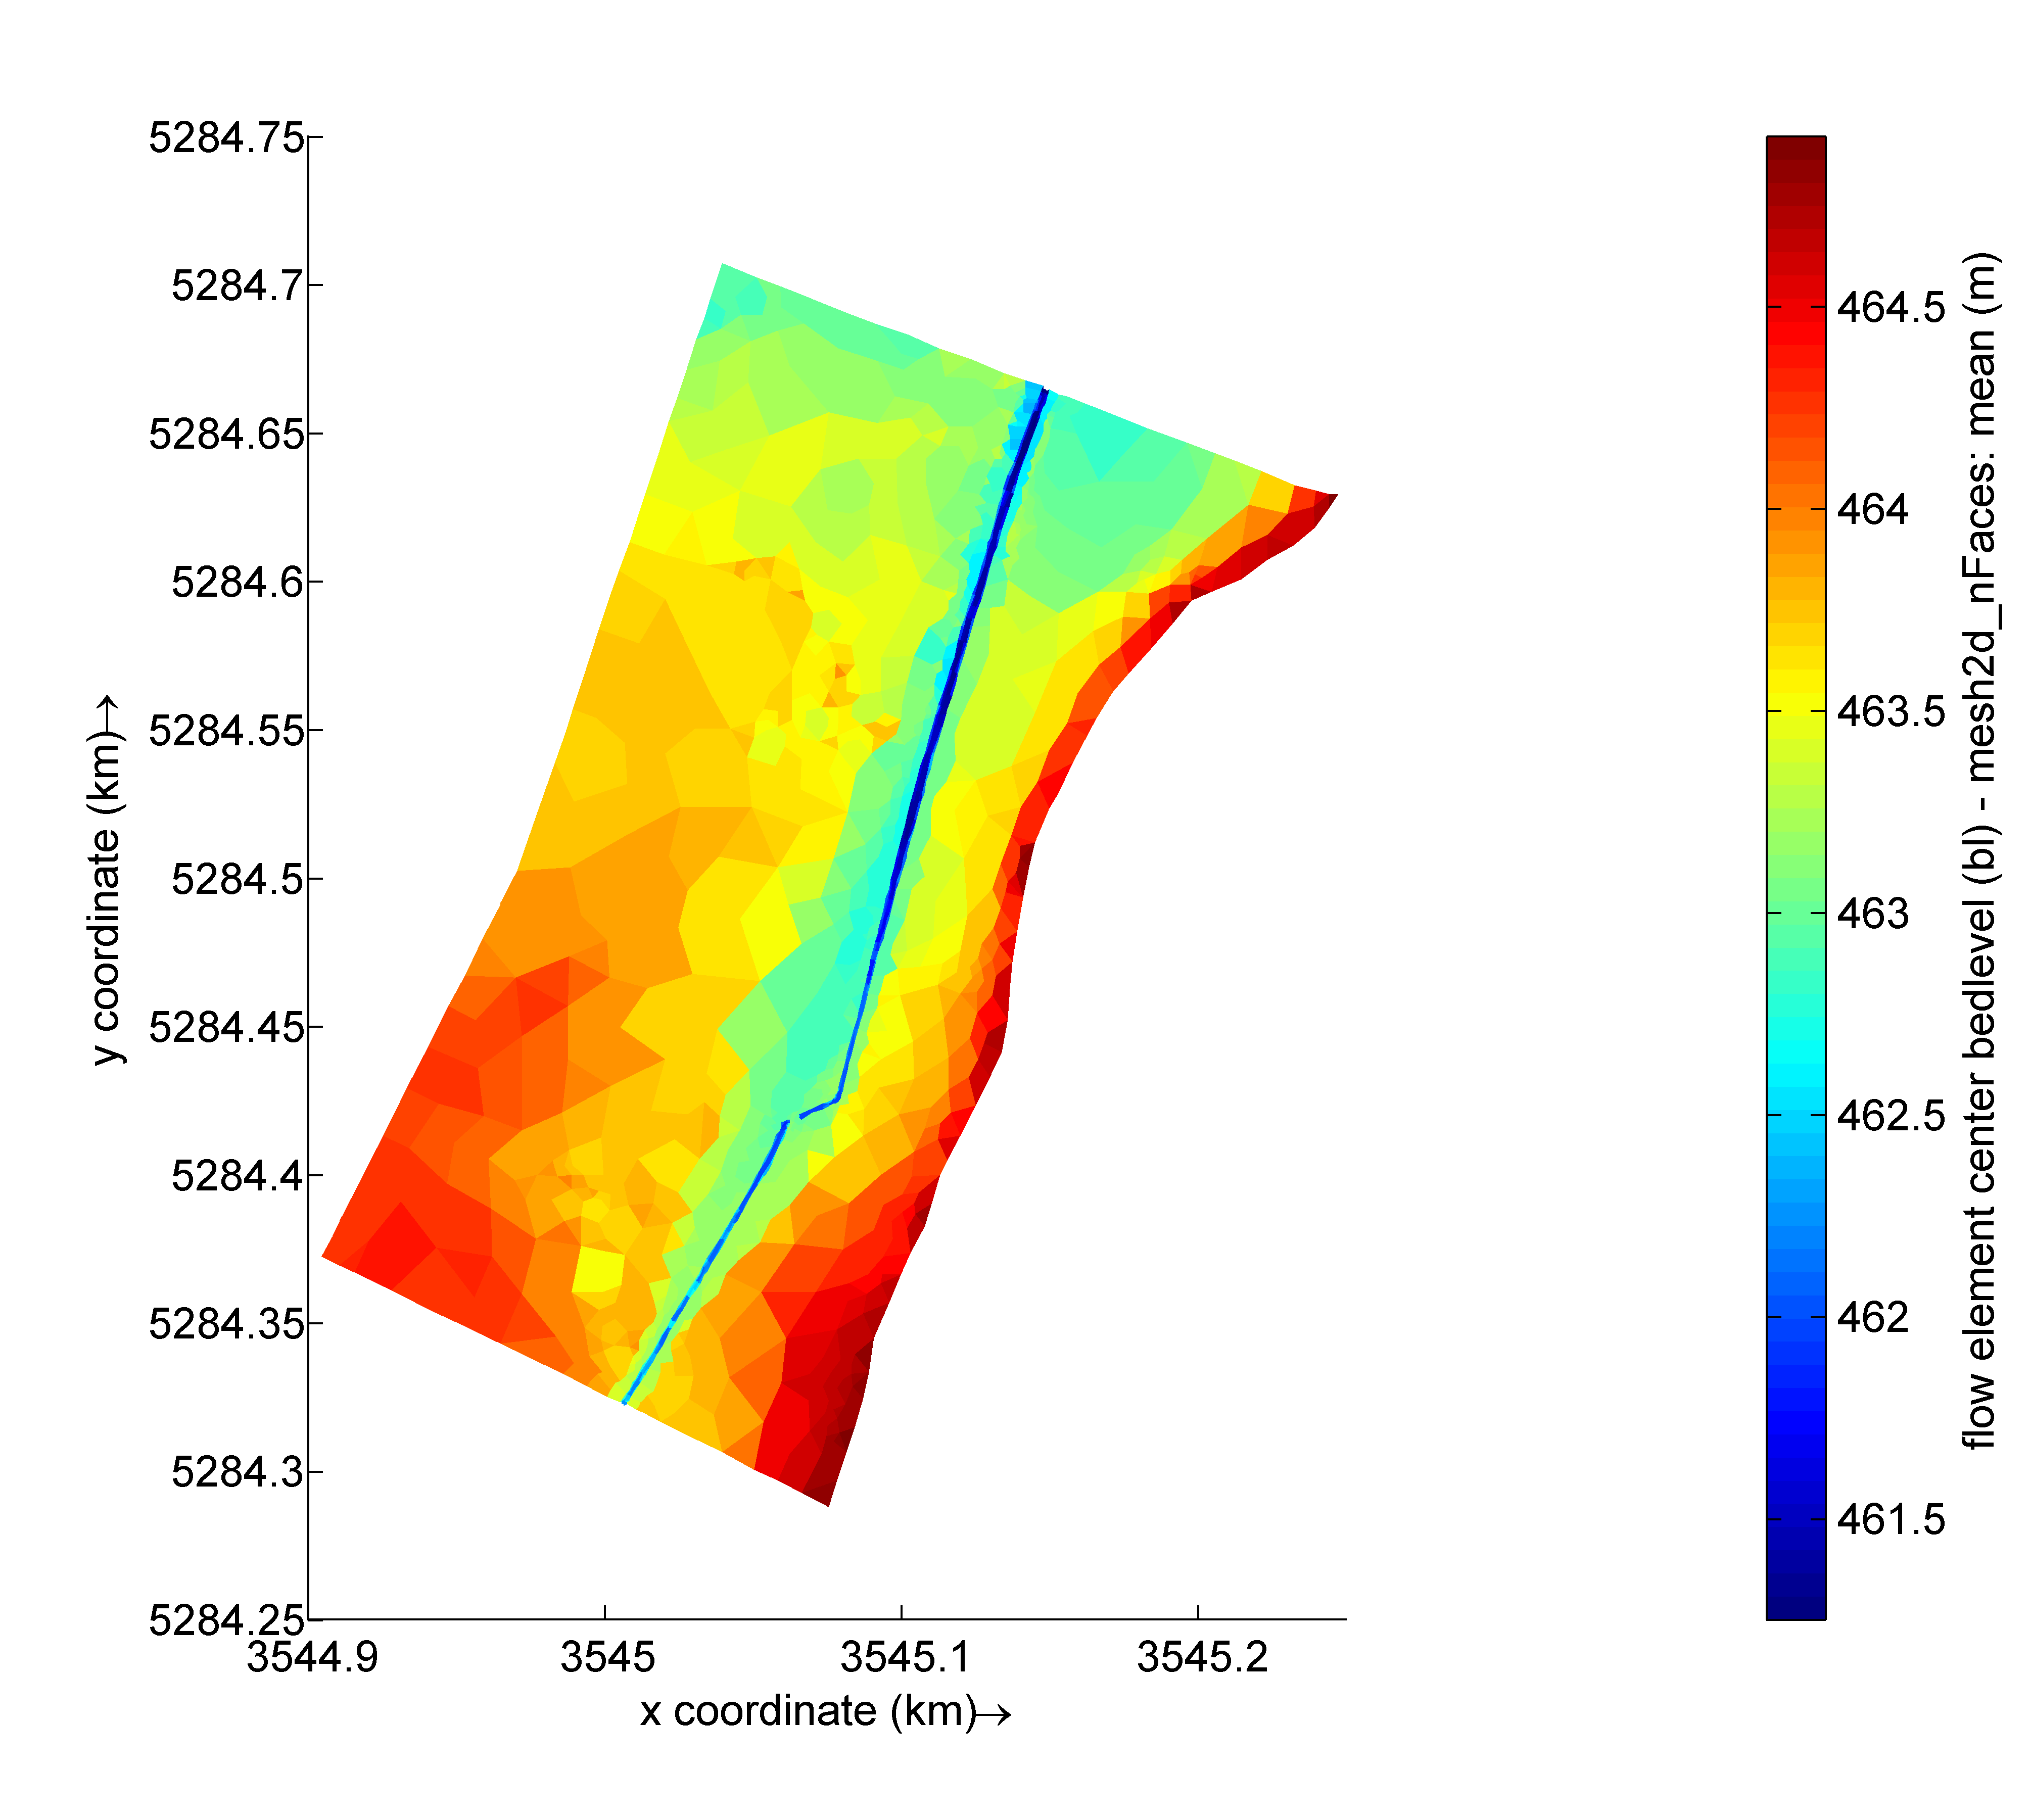
\includegraphics[scale=0.8]{PICTURES/models_ini/bed_levels.png}
    \caption{Surface Elevation of the Model Grid.}
    \label{fig:grid_bed_levels}
\end{figure}

\section{Model Parameters and Regular Inputs}
This section mentions the inputs and parameters used for the models and briefly discusses the rationale for using the same, if necessary.

\subsection{GWSWEX}
Refer \ref{GWSWEX_input}.
\begin{itemize}
    \item precipitation influxes are obtained from the German Weather Service (DWD) for the station \textit{Weingarten, Ravensburg}.
    \item evapotranspiration outfluxes are obtained from previous calculations in the parent study.
    \item n is linked to the specific yield of the unconfined aquifer set in the GW model.
    \item n\textunderscore gw is linked to the specific storage of the unconfined aquifer set in the GW model,
    \item m = 0.3, decided as an initial guess.
    \item k is linked to the hydraulic conductivity of the unconfined aquifer set in the GW model.
    \item $\alpha$ = 0.15, decided as an initial guess.
    \item $\beta$ = 0.7, decided as an initial guess.
    \item $SW_th$ = 0.05, decided as an initial guess based on the ET fluxes and the local simulation time period.
\end{itemize}

\subsection{Modflow 6}
The GW model is set up on Modflow 6 (refer \ref{mf6}) in accordance with the hydrogeological properties as illustrated in \ref{fig:wasenmoosCS}. The top of the model corresponds to the ground surface elevation. The bottom of the unconfined aquifer is set to the lowest elevation of the stream. It is to be assessed if this is an adequately realistic representation of reality. Figure \ref{fig:aq0_thickness} shows the thickness of the unconfined aquifer over the model grid. The aquitard layer and the confined layer are assumed to be uniformly thick, each bearing a thickness of \unit[1]{m} and \unit[10]{m} respectively.

\begin{figure}[h!]
    \centering
    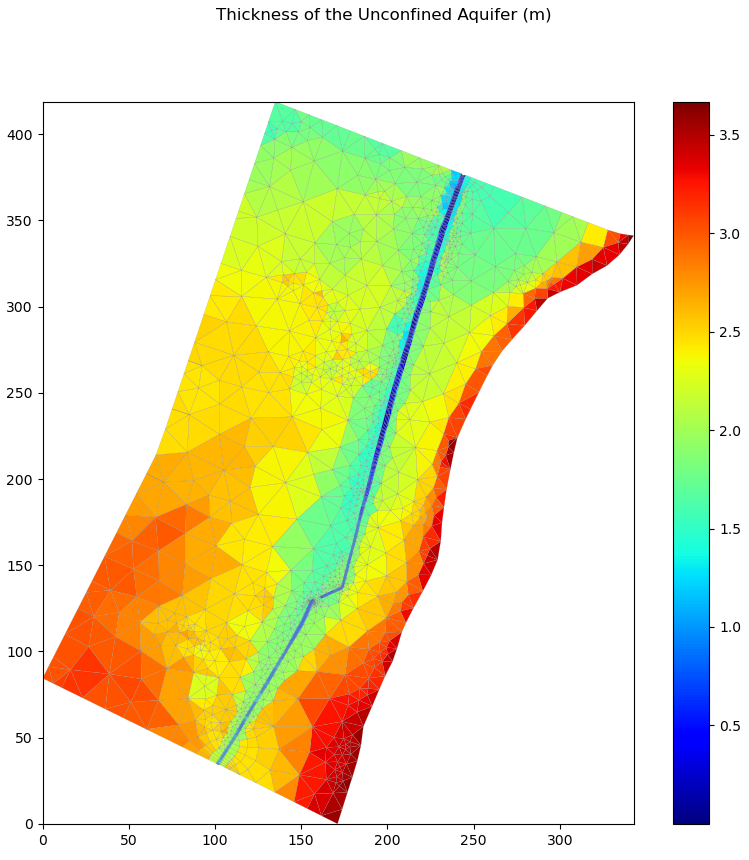
\includegraphics[scale=0.42]{PICTURES/models_ini/aq0_thickness.png}
    \caption{Thickness of the Unconfined Aquifer (m).}
    \label{fig:aq0_thickness}
\end{figure}

The assumptions for hydraulic conductivities ($K$), specific yields ($S_y$), and specific storages ($S_s$) for the three layers, based on peer-reviewed literature are as follows \cite{Rezanezhad2016} \cite{Lennartz} \cite{Lu2015} \cite{Shestakov2002} \cite{Schlotzhauer1999}:
\begin{table}[h!]
\caption{Assumed hydrogeological properties}
\label{tab:hydrogeoIP}
\centering
\begin{tabular}{llll}
\hline\noalign{\smallskip}
aquifer & $K$ & $S_y$ & $S_s$  \\
\noalign{\smallskip}\hline\noalign{\smallskip}
unconfined aquifer & \SI{5e-4}{\meter\per\second} & 0.4 & \SI{6e-3}{\per\meter} \\
clay aquitard & \SI{3e-9}{\meter\per\second} & 0.15 & \SI{1e-3}{\per\meter} \\
confined aquifer & \SI{1e-4}{\meter\per\second} & 0.15 & \SI{2e-5}{\per\meter} \\
\noalign{\smallskip}\hline
\end{tabular}
\end{table}

\subsection{D-Flow FM}
The setup of the SW model is rather quite simple, stemming partially from the fact that the SW processes and storages are not very dominant in this study in comparison to the GW storages and processes, and partially from the undemanding nature of required model parameters to set up the D-Flow FM model.
\\
The Manning's coefficient is set to 0.23 over the model domain and to 0.05 at the stream.

\section{Initial Conditions}

\subsection{GWSWEX}
The initial GW and SW levels are read from the GW and SW models respectively. Initial SM levels are set to 80\% saturation of the ePV. It is to be assessed whether this is a adequately realistic assumption.
\begin{figure}[!h]
\minipage{0.5\textwidth}
  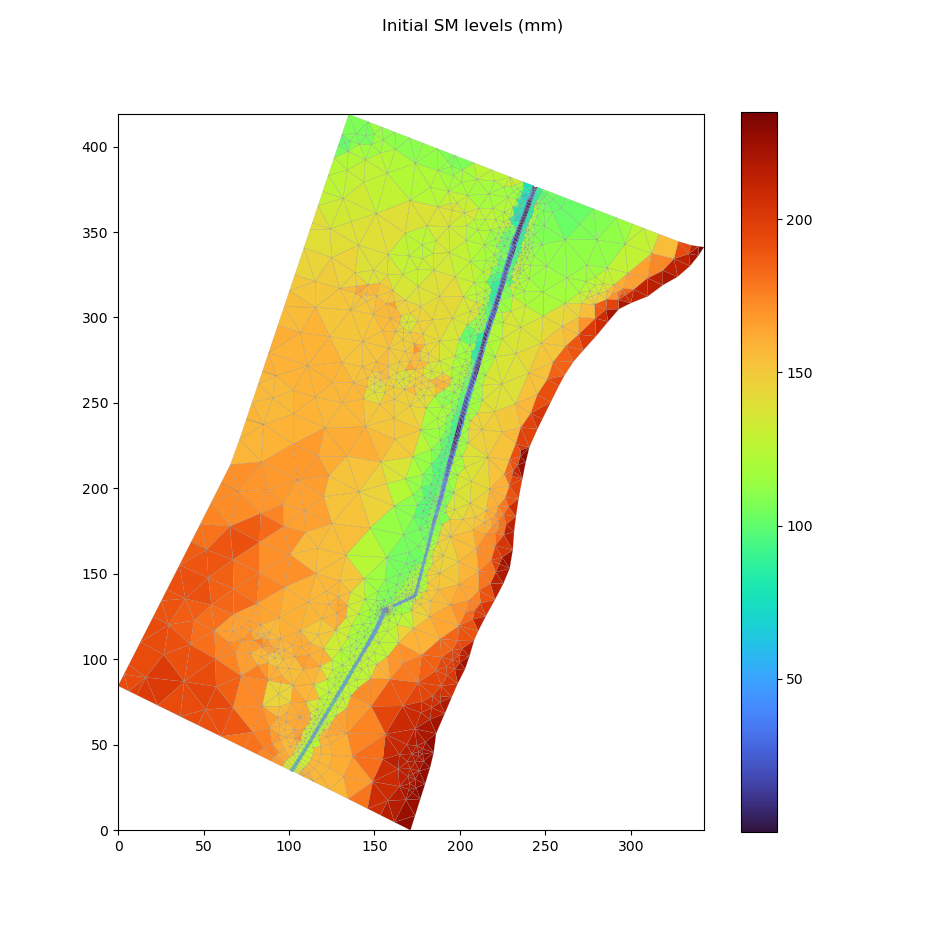
\includegraphics[width=\linewidth]{PICTURES/models_ini/sm_ini}
\endminipage\hfill
\minipage{0.5\textwidth}
  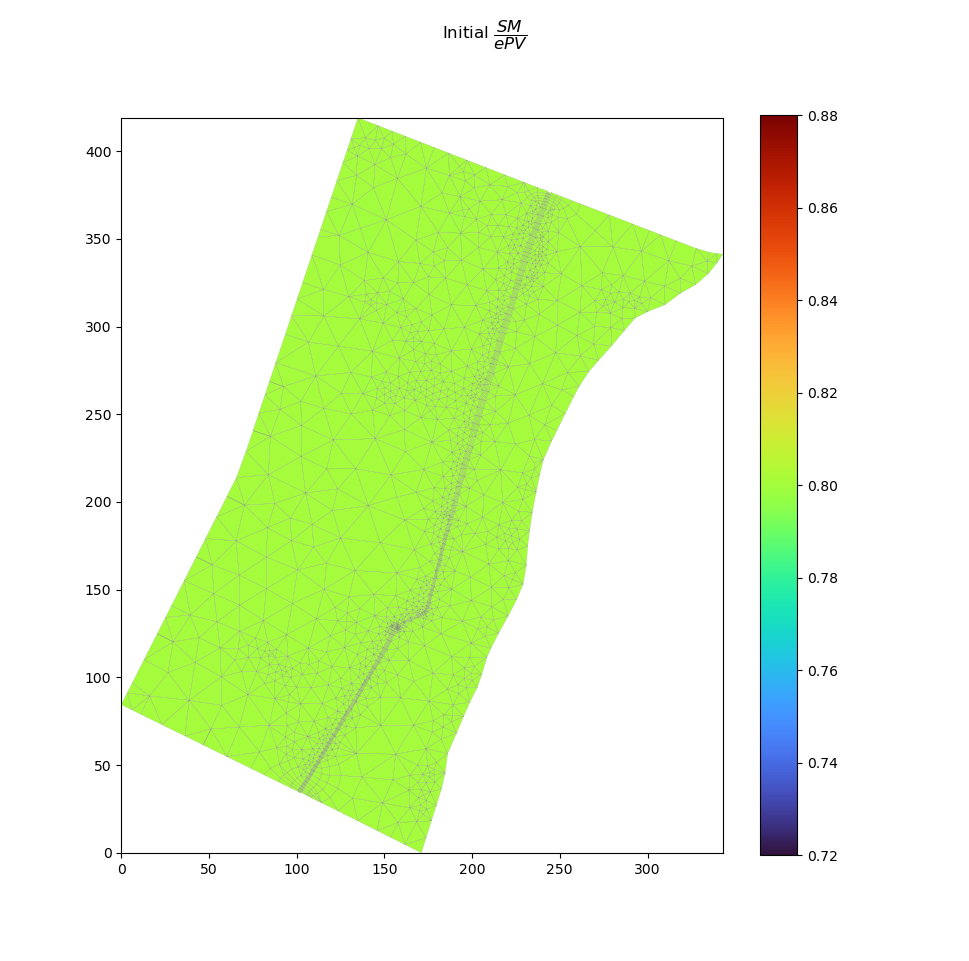
\includegraphics[width=\linewidth]{PICTURES/models_ini/sm_ini_ratio}
\endminipage\hfill
\caption{Initial soil moisture: left - absolute levels (mm); right - relative saturation.}\label{fig:sm_ini}
\end{figure}

\subsection{Modflow 6}
The starting heads for the unconfined aquifer was set to 80\% saturation. This corresponds to the GW level observed in observation point P-7 (refer Figure \ref{fig:obs_pts} for location). This way, the heads would correspond to the trends of the surface elevation. The starting heads for the aquitard and the confined aquifer are set at \unit[0.1]{m} above the model top elevation. It is to be assessed how these assumptions hold true.

\begin{figure}[!h]
\minipage{0.32\textwidth}
  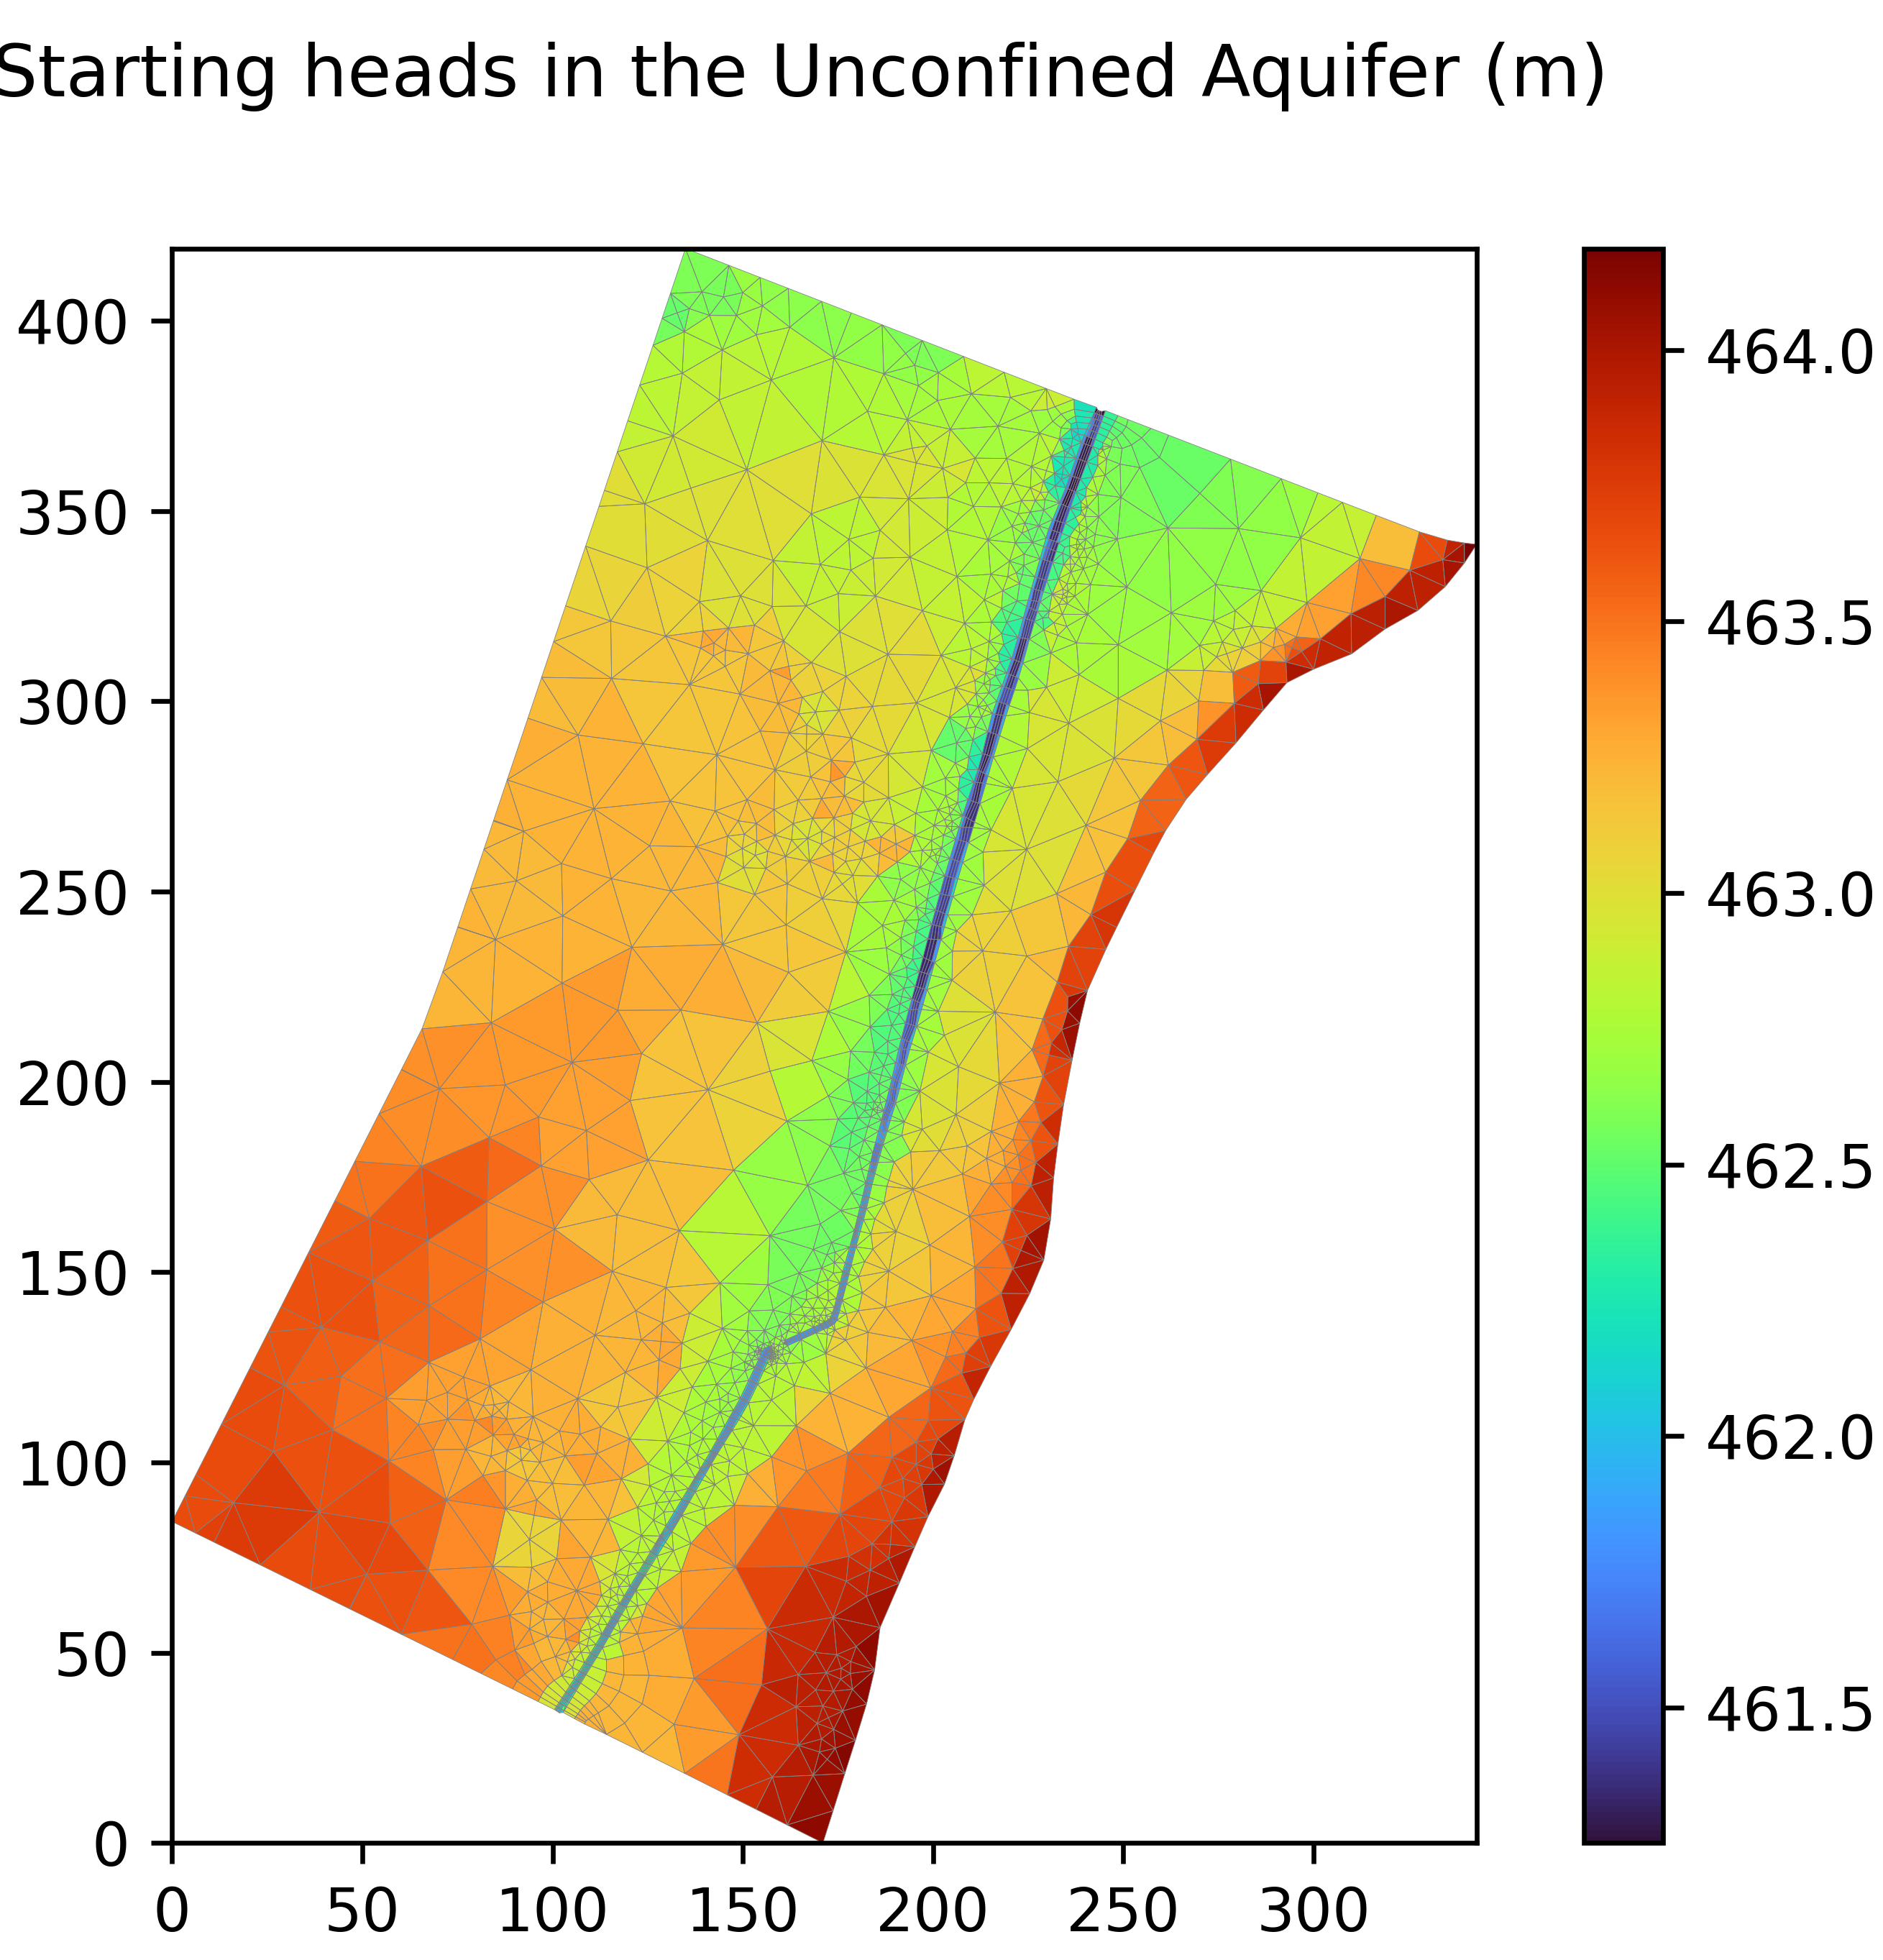
\includegraphics[width=\linewidth]{PICTURES/models_ini/strt_aq0}
\endminipage\hfill
\minipage{0.32\textwidth}
  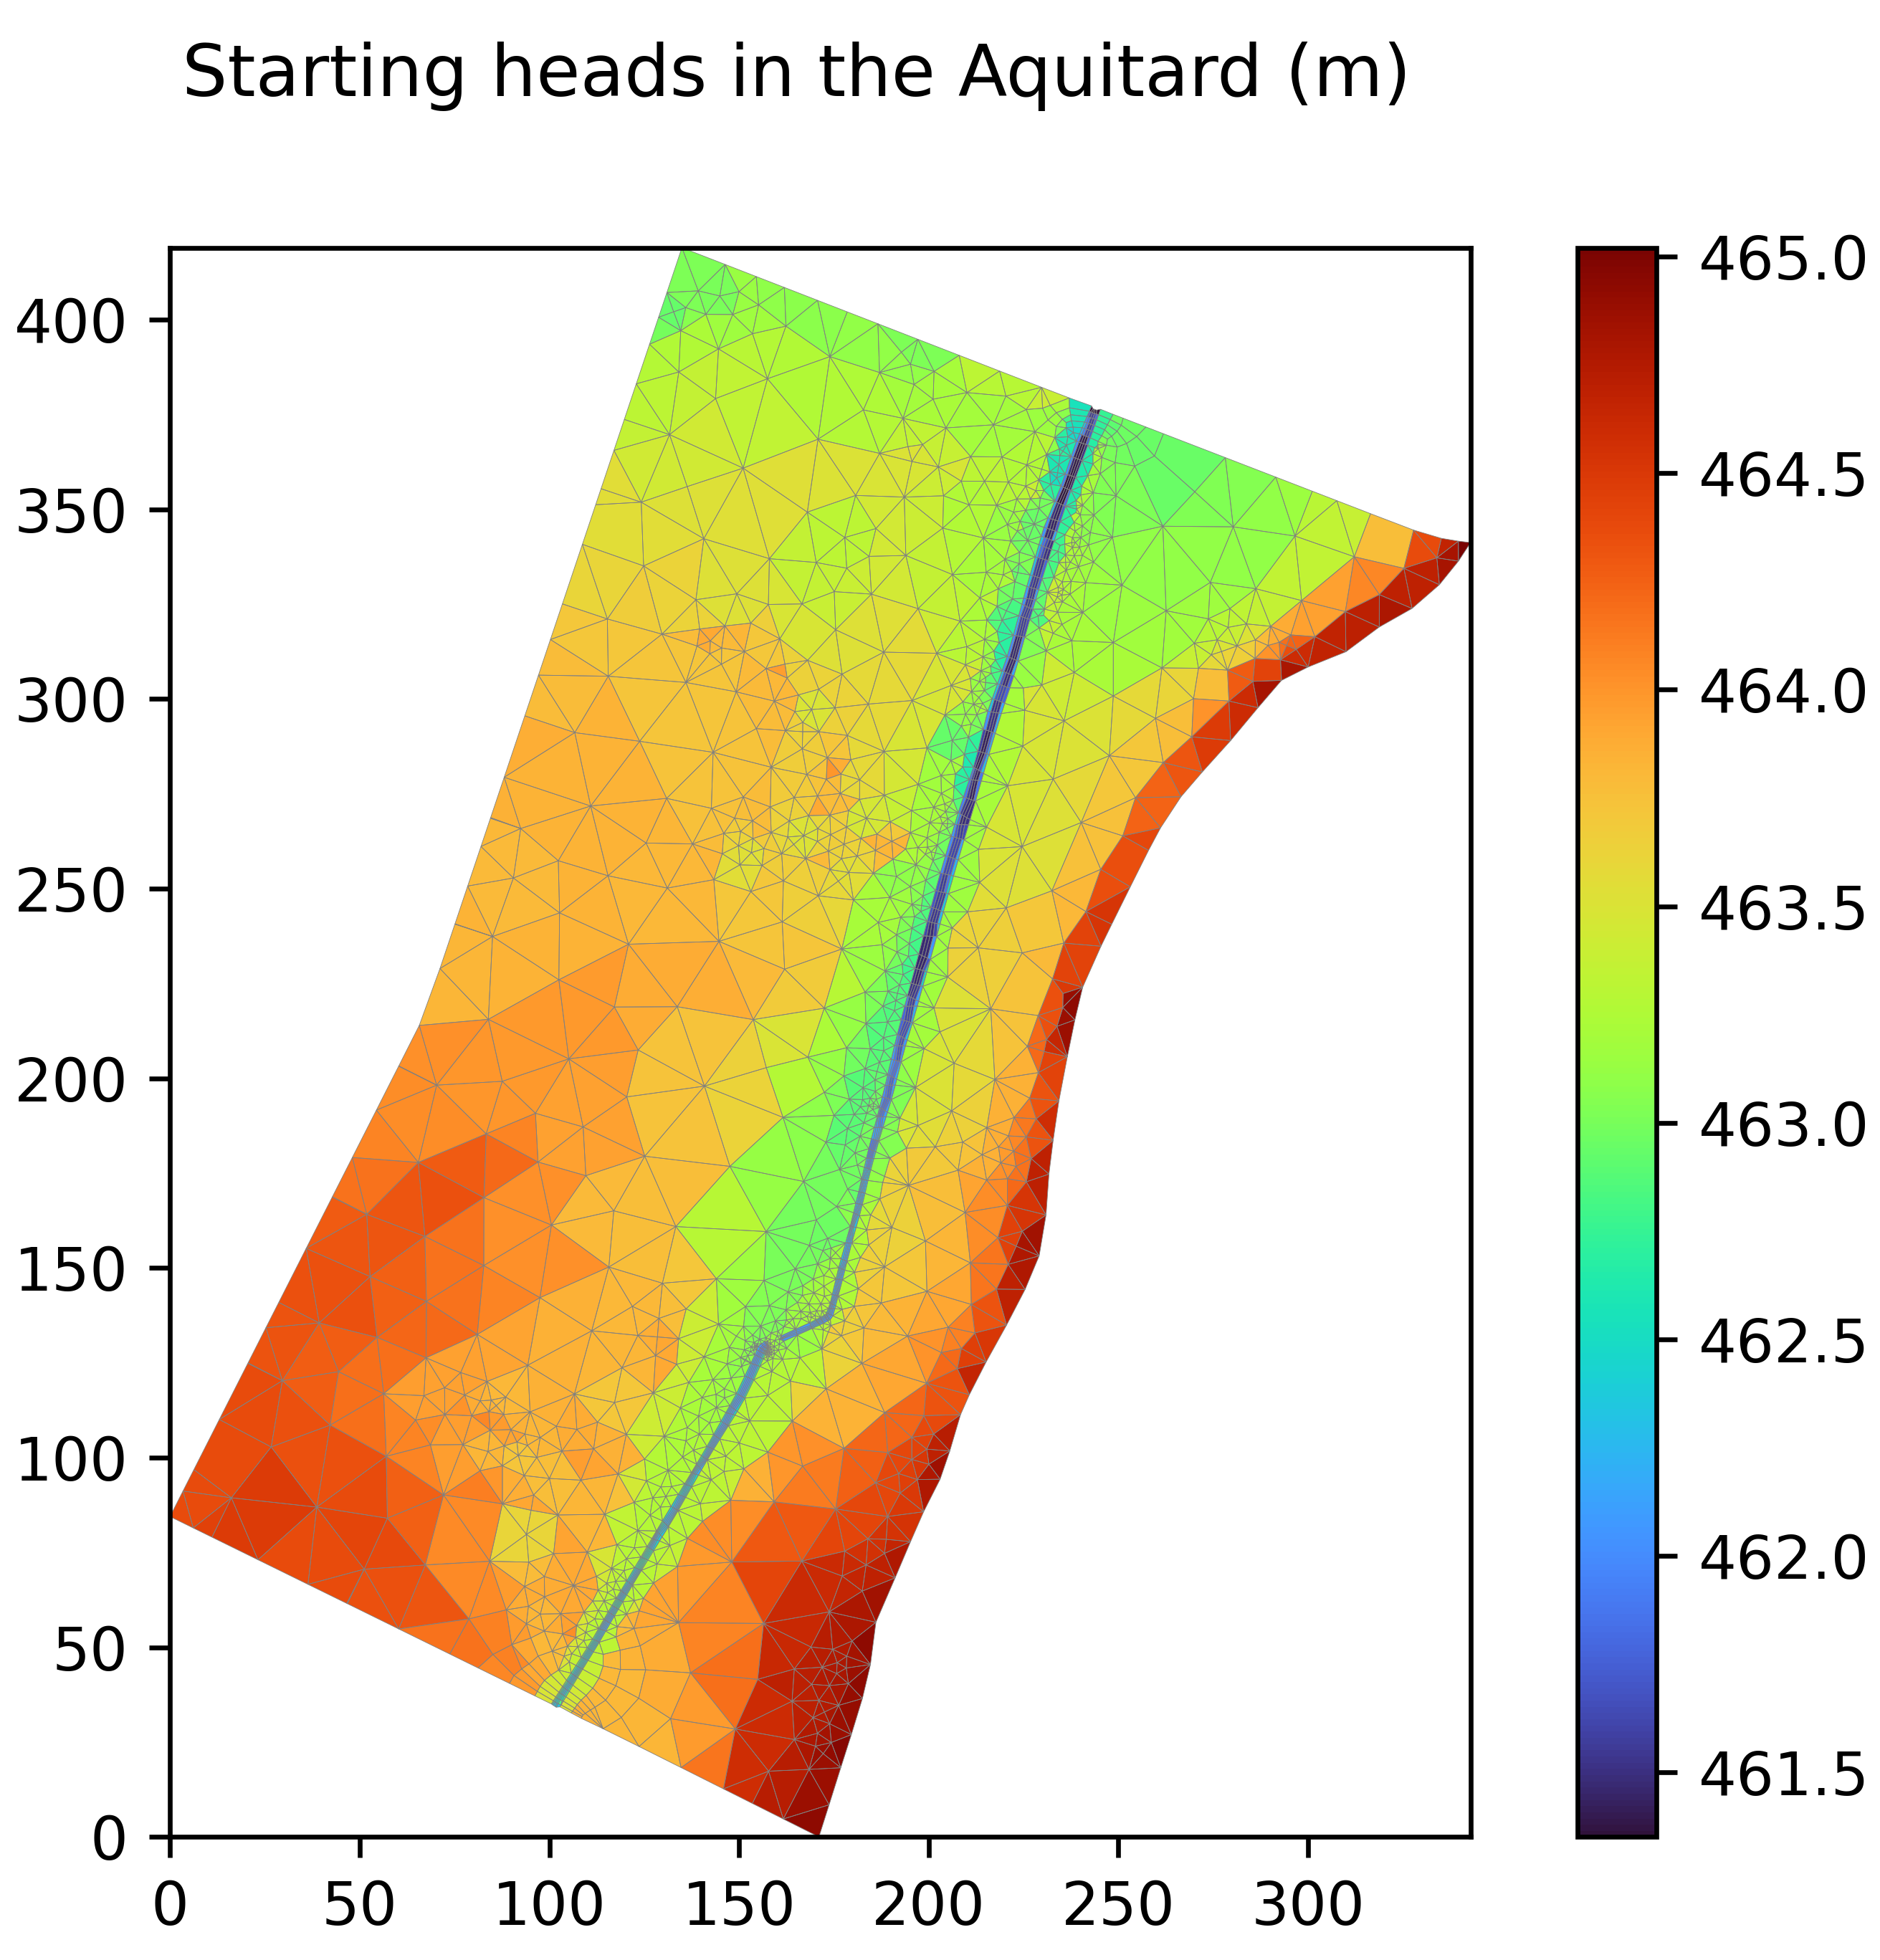
\includegraphics[width=\linewidth]{PICTURES/models_ini/strt_aq1}
\endminipage\hfill
\minipage{0.32\textwidth}
  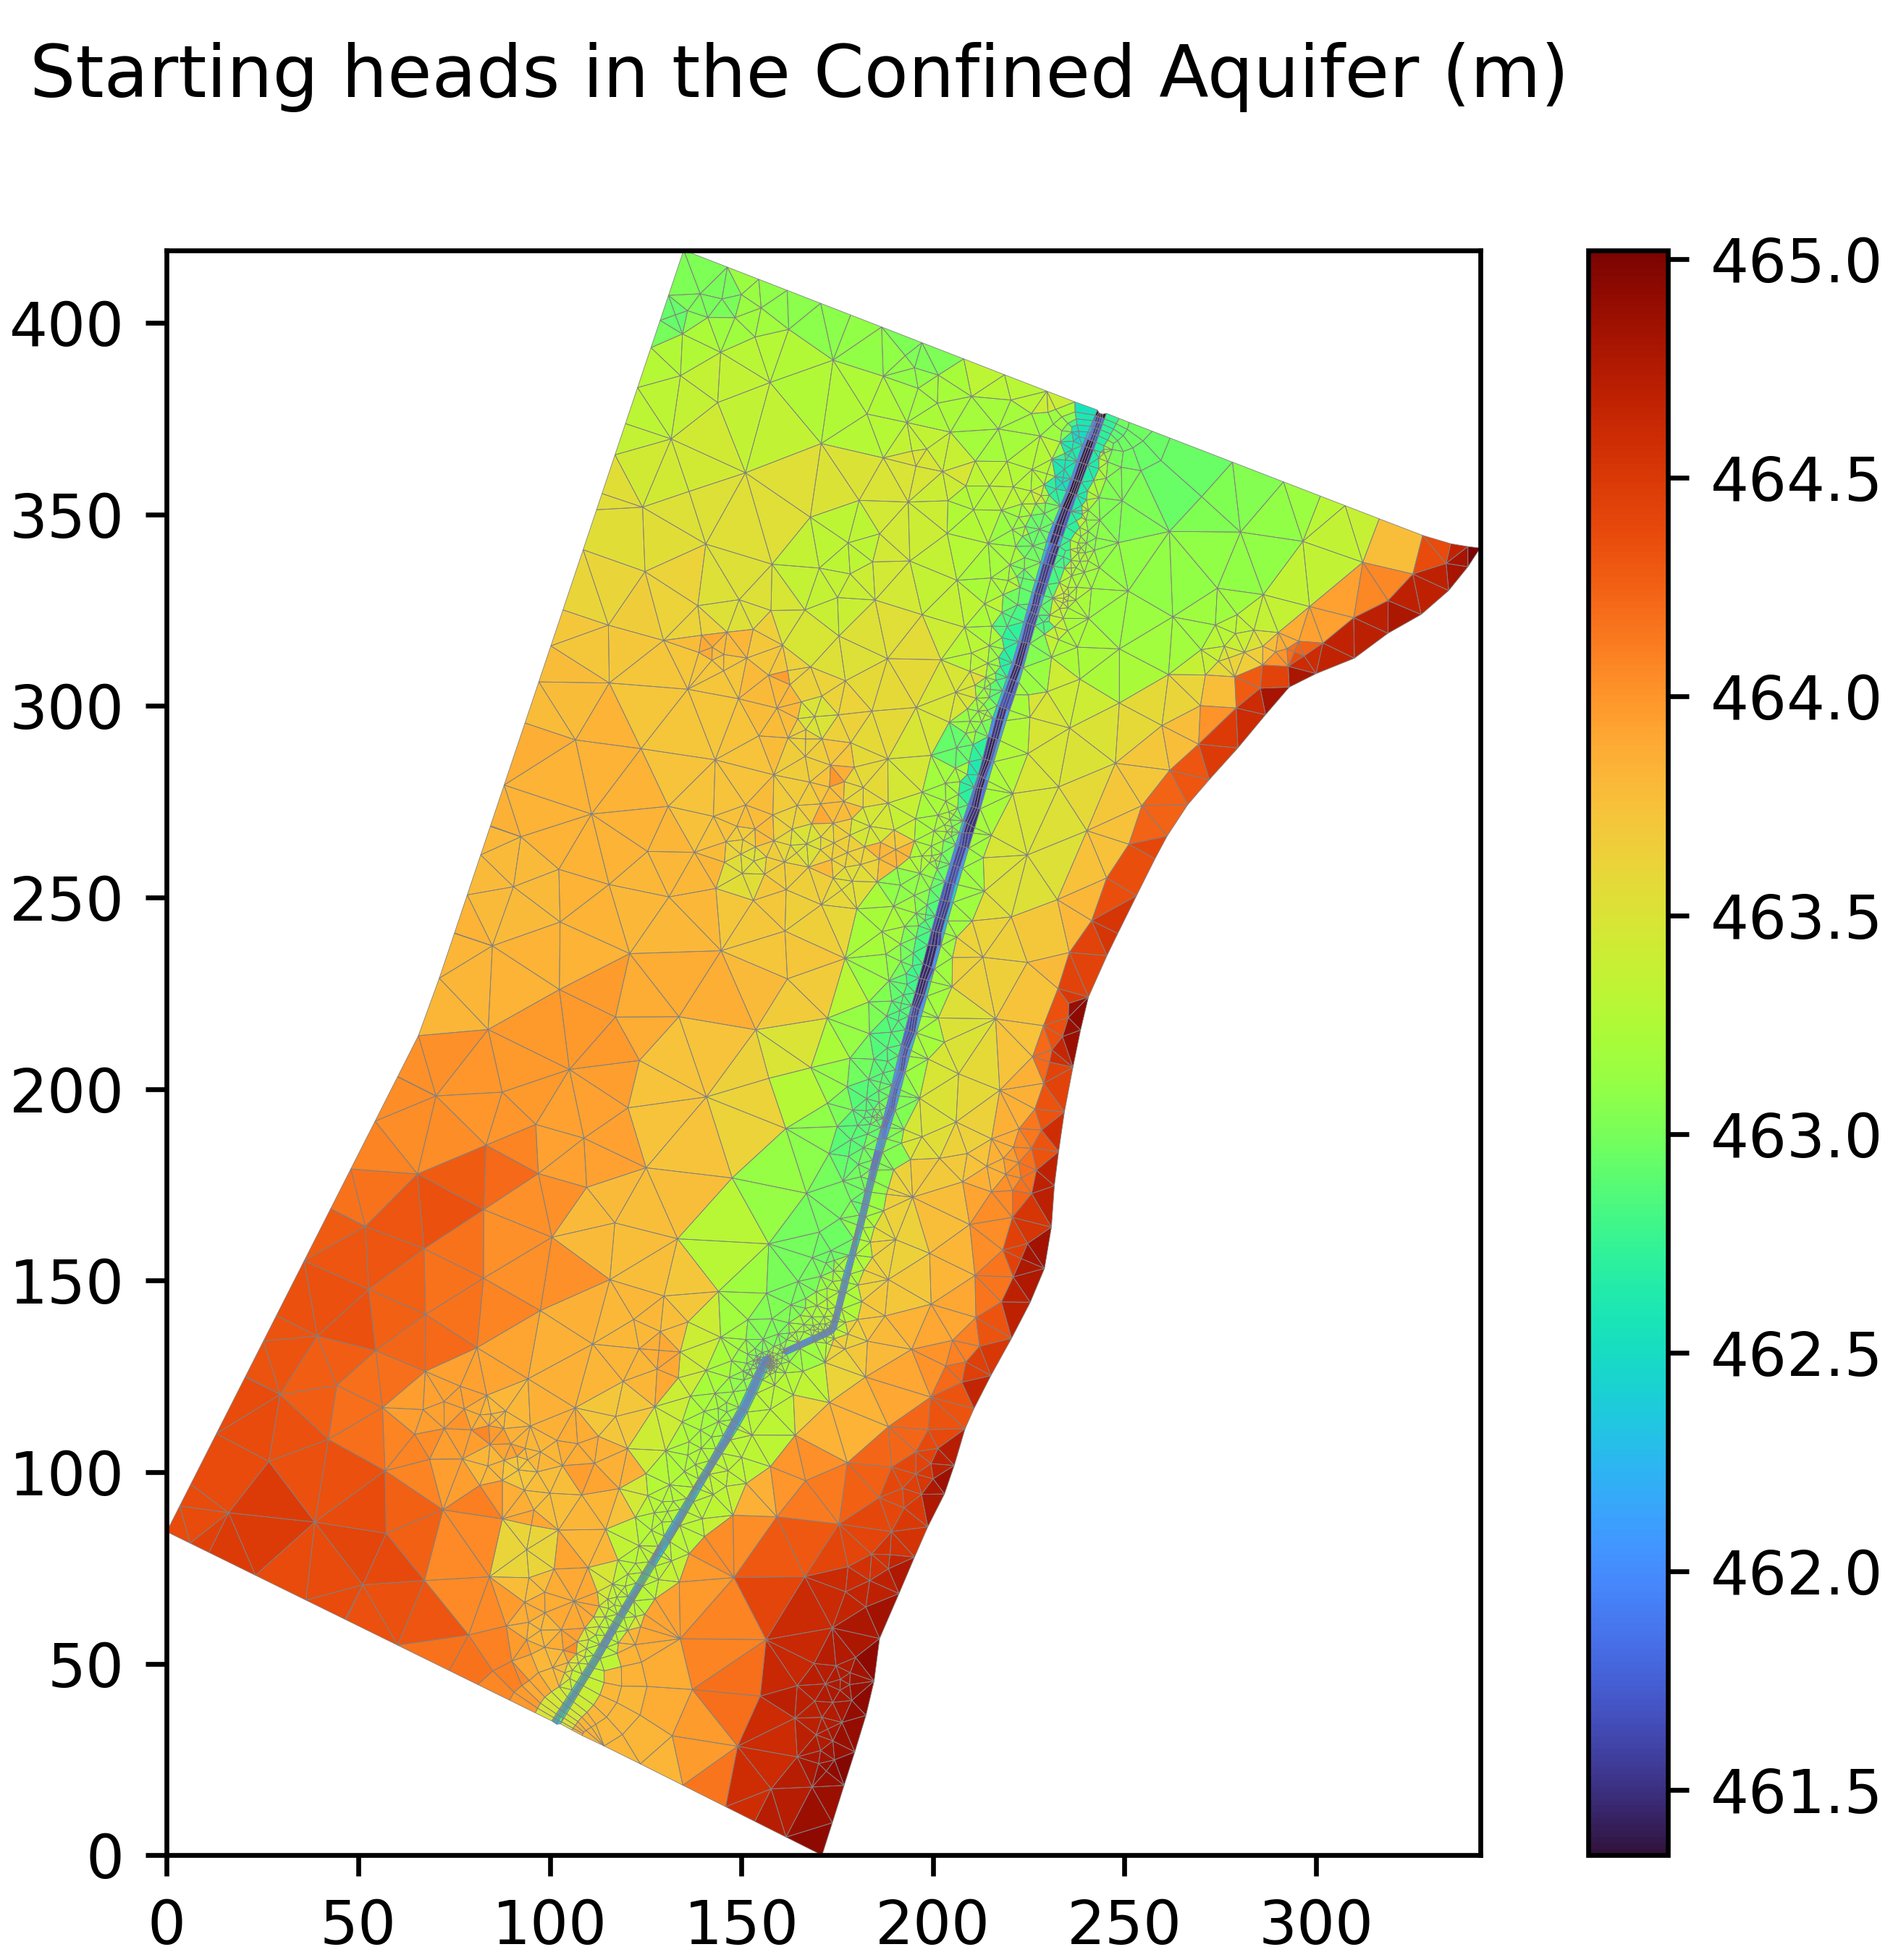
\includegraphics[width=\linewidth]{PICTURES/models_ini/strt_aq2}
\endminipage
\caption{Starting heads in the GW Model.}\label{fig:mf6_ic_strt}
\end{figure}

\subsection{D-Flow FM}
Initial water levels just adequate for all model cells to be considered wet are prescribed as starting water levels in the SW model. This is expected to correspond to reality as the system is not SW dominant and precipitation influx right before the start of the simulation period is sparse.

\begin{figure}[h!]
    \centering
    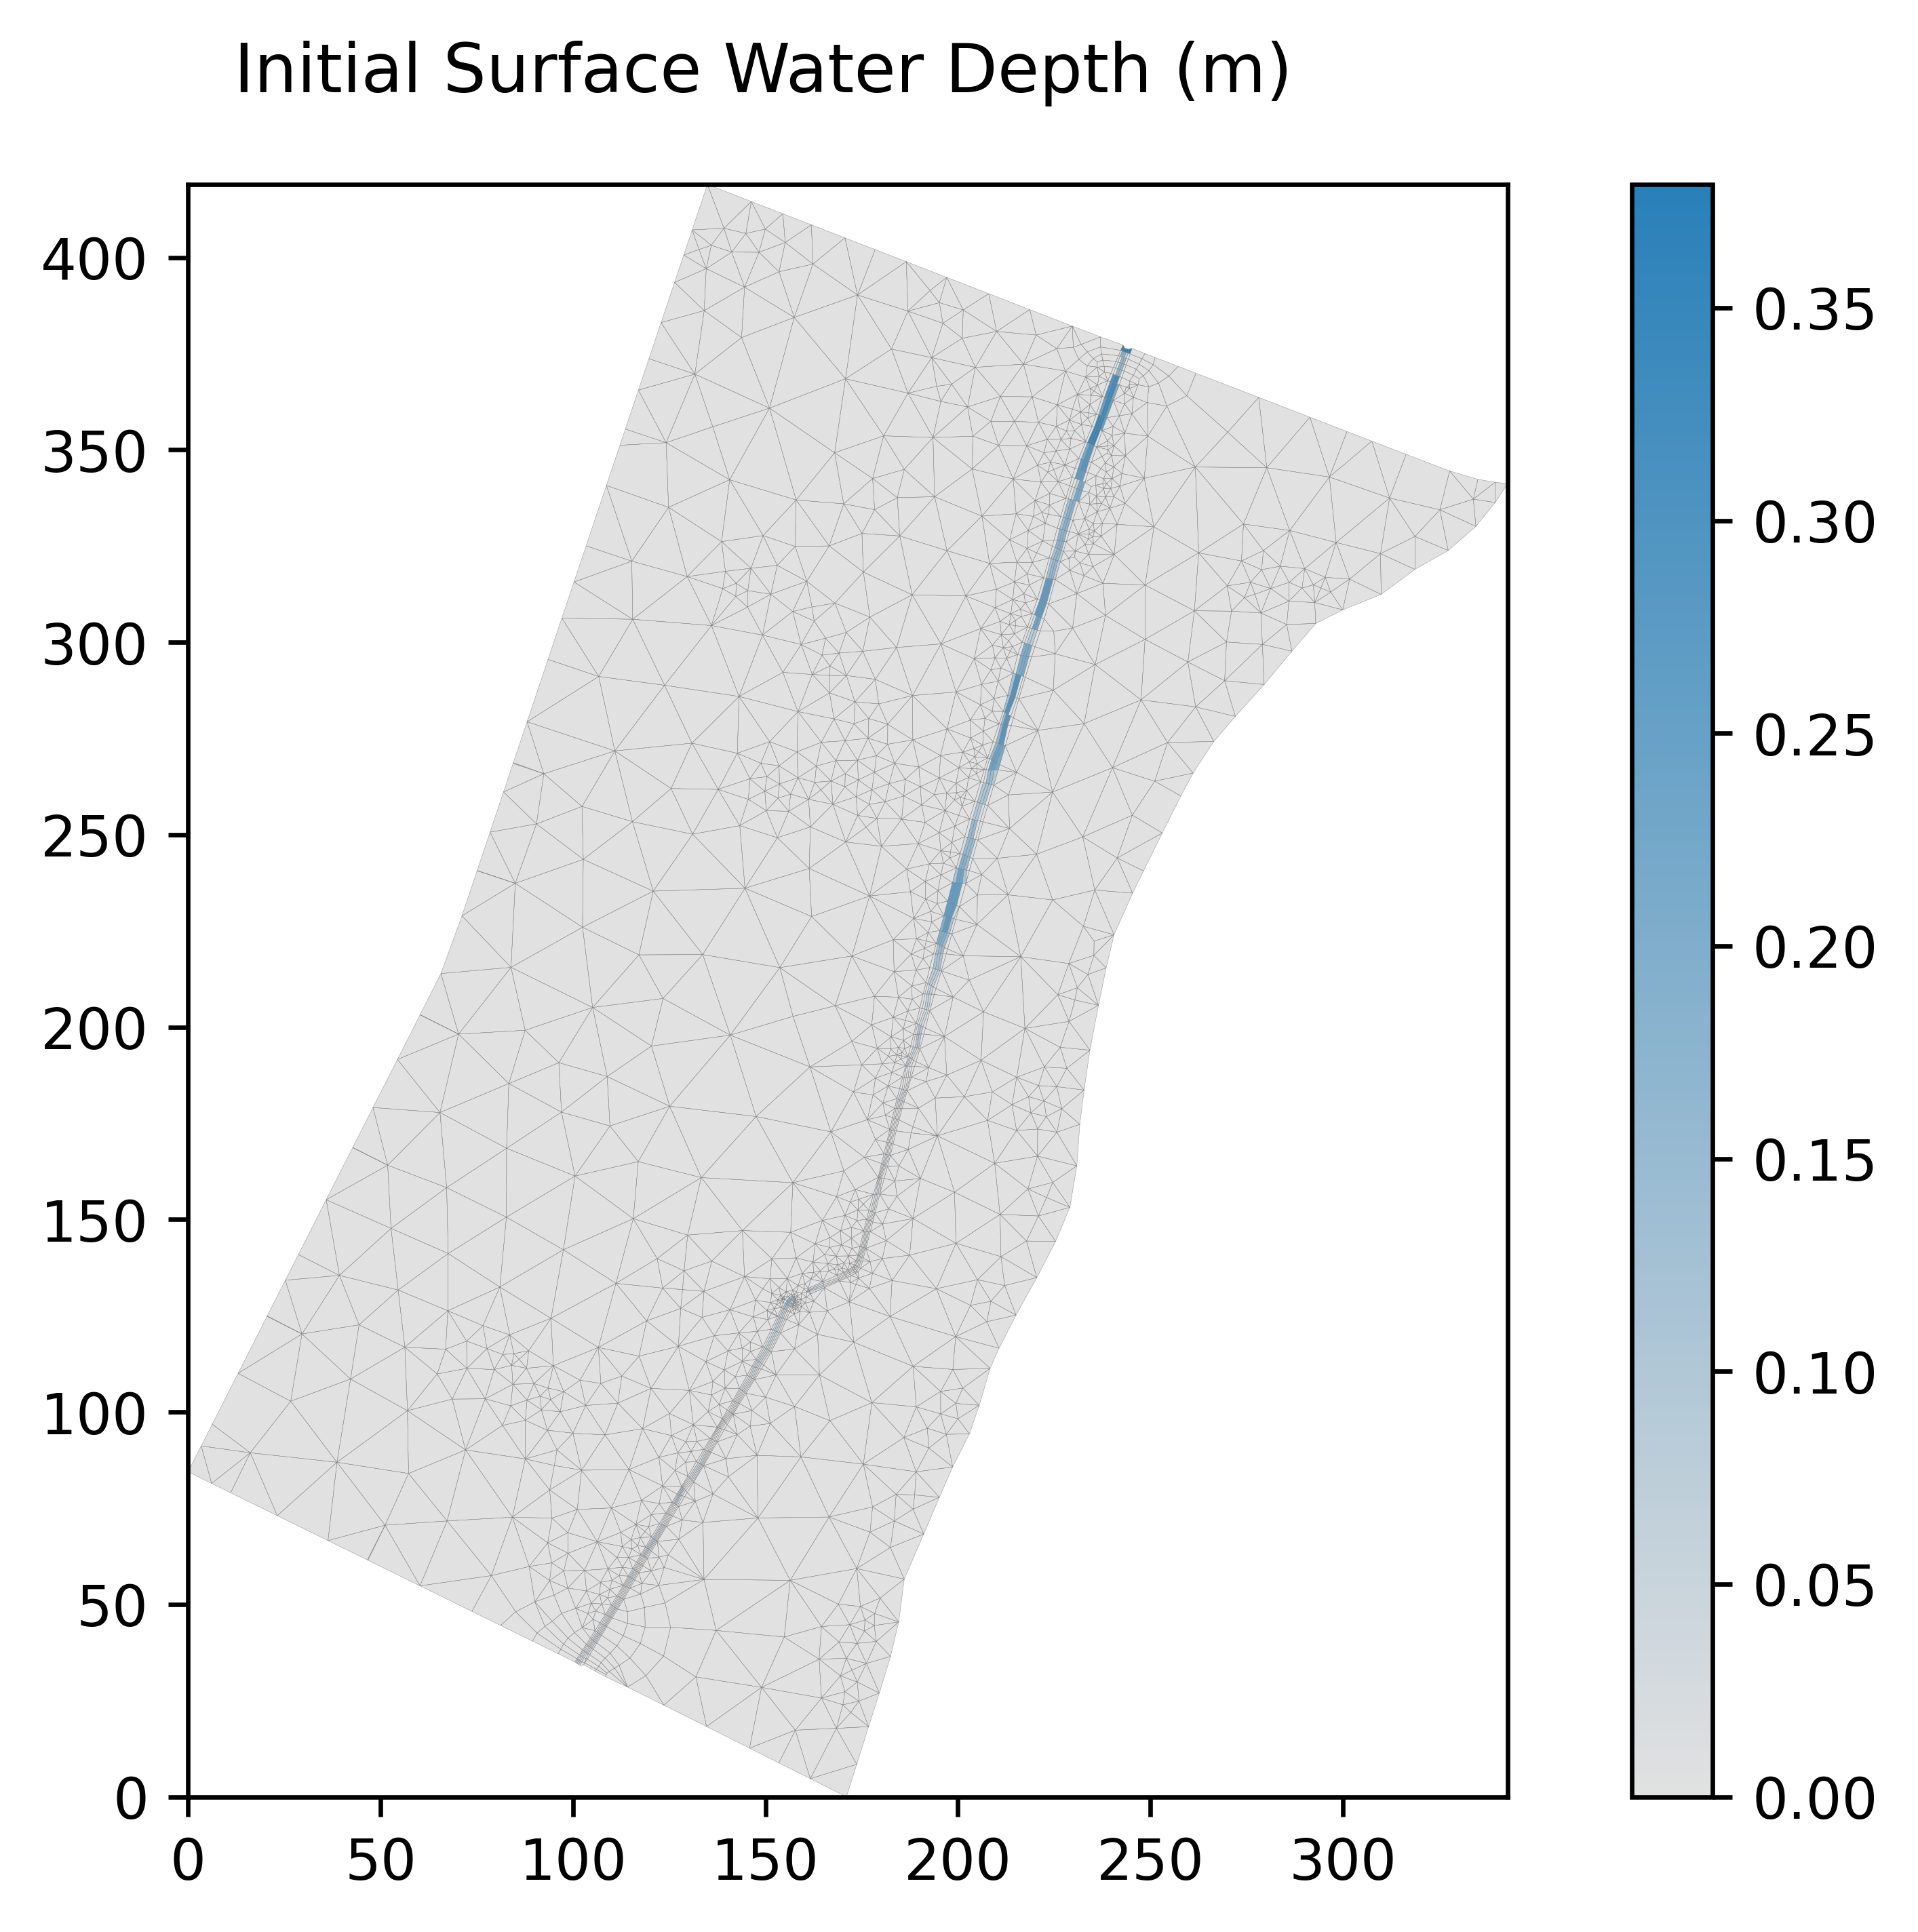
\includegraphics[scale=1]{PICTURES/models_ini/sws_ini.png}
    \caption{Initial Surface Water levels.}
    \label{fig:delft_iniWL}
\end{figure}


\section{Boundary Conditions}

\subsection{GWSWEX}
Grid elements that are bound by constant-head (CHD) boundary conditions in the GW model are flagged in the GWSWEX model so that the numerical scheme does not try to alter the GW heads, as observed by the illustration of the numerical scheme in Figure \ref{fig:GWSWEX_flow}.

\subsection{Modflow 6}
A constant head (CHD) boundary for the confined aquifer is set along the eastern boundary of the model grid as seen in Figure \ref{fig:grid_qgis}. The heads here are set to the surface level elevation based on speculation. \\
Along the stream, a CHD boundary is set in grid elements of the unconfined aquifer in locations that exhibit the presence of surface-water in the SW model at the end of the previous local simulation period. This boundary condition is thus dynamically updated every local simulation period with water levels read from the SW model.

\subsection{D-Flow FM}
A water level boundary condition is enforced along the northern-most grid elements in the stream, as seen by the elements marked by red in this area in Figure \ref{fig:grid_qgis}. The water levels for this enforcement is obtained from a water level observation at this location in the study area. Thus, with this enforcement, the initial water level in the SW model is as illustrated in Figure \ref{fig:delft_iniWL}.


\section{Observations}
Figure \ref{fig:obs_pts} shows the locations of GW observations located in the model domain. An SW observation is located as described in the previous section. However, since data from that observation is directly used to enforce a boundary condition in the SW model, it is of no relevance to compare model results to measured observations.

\begin{figure}[h!]
    \centering
    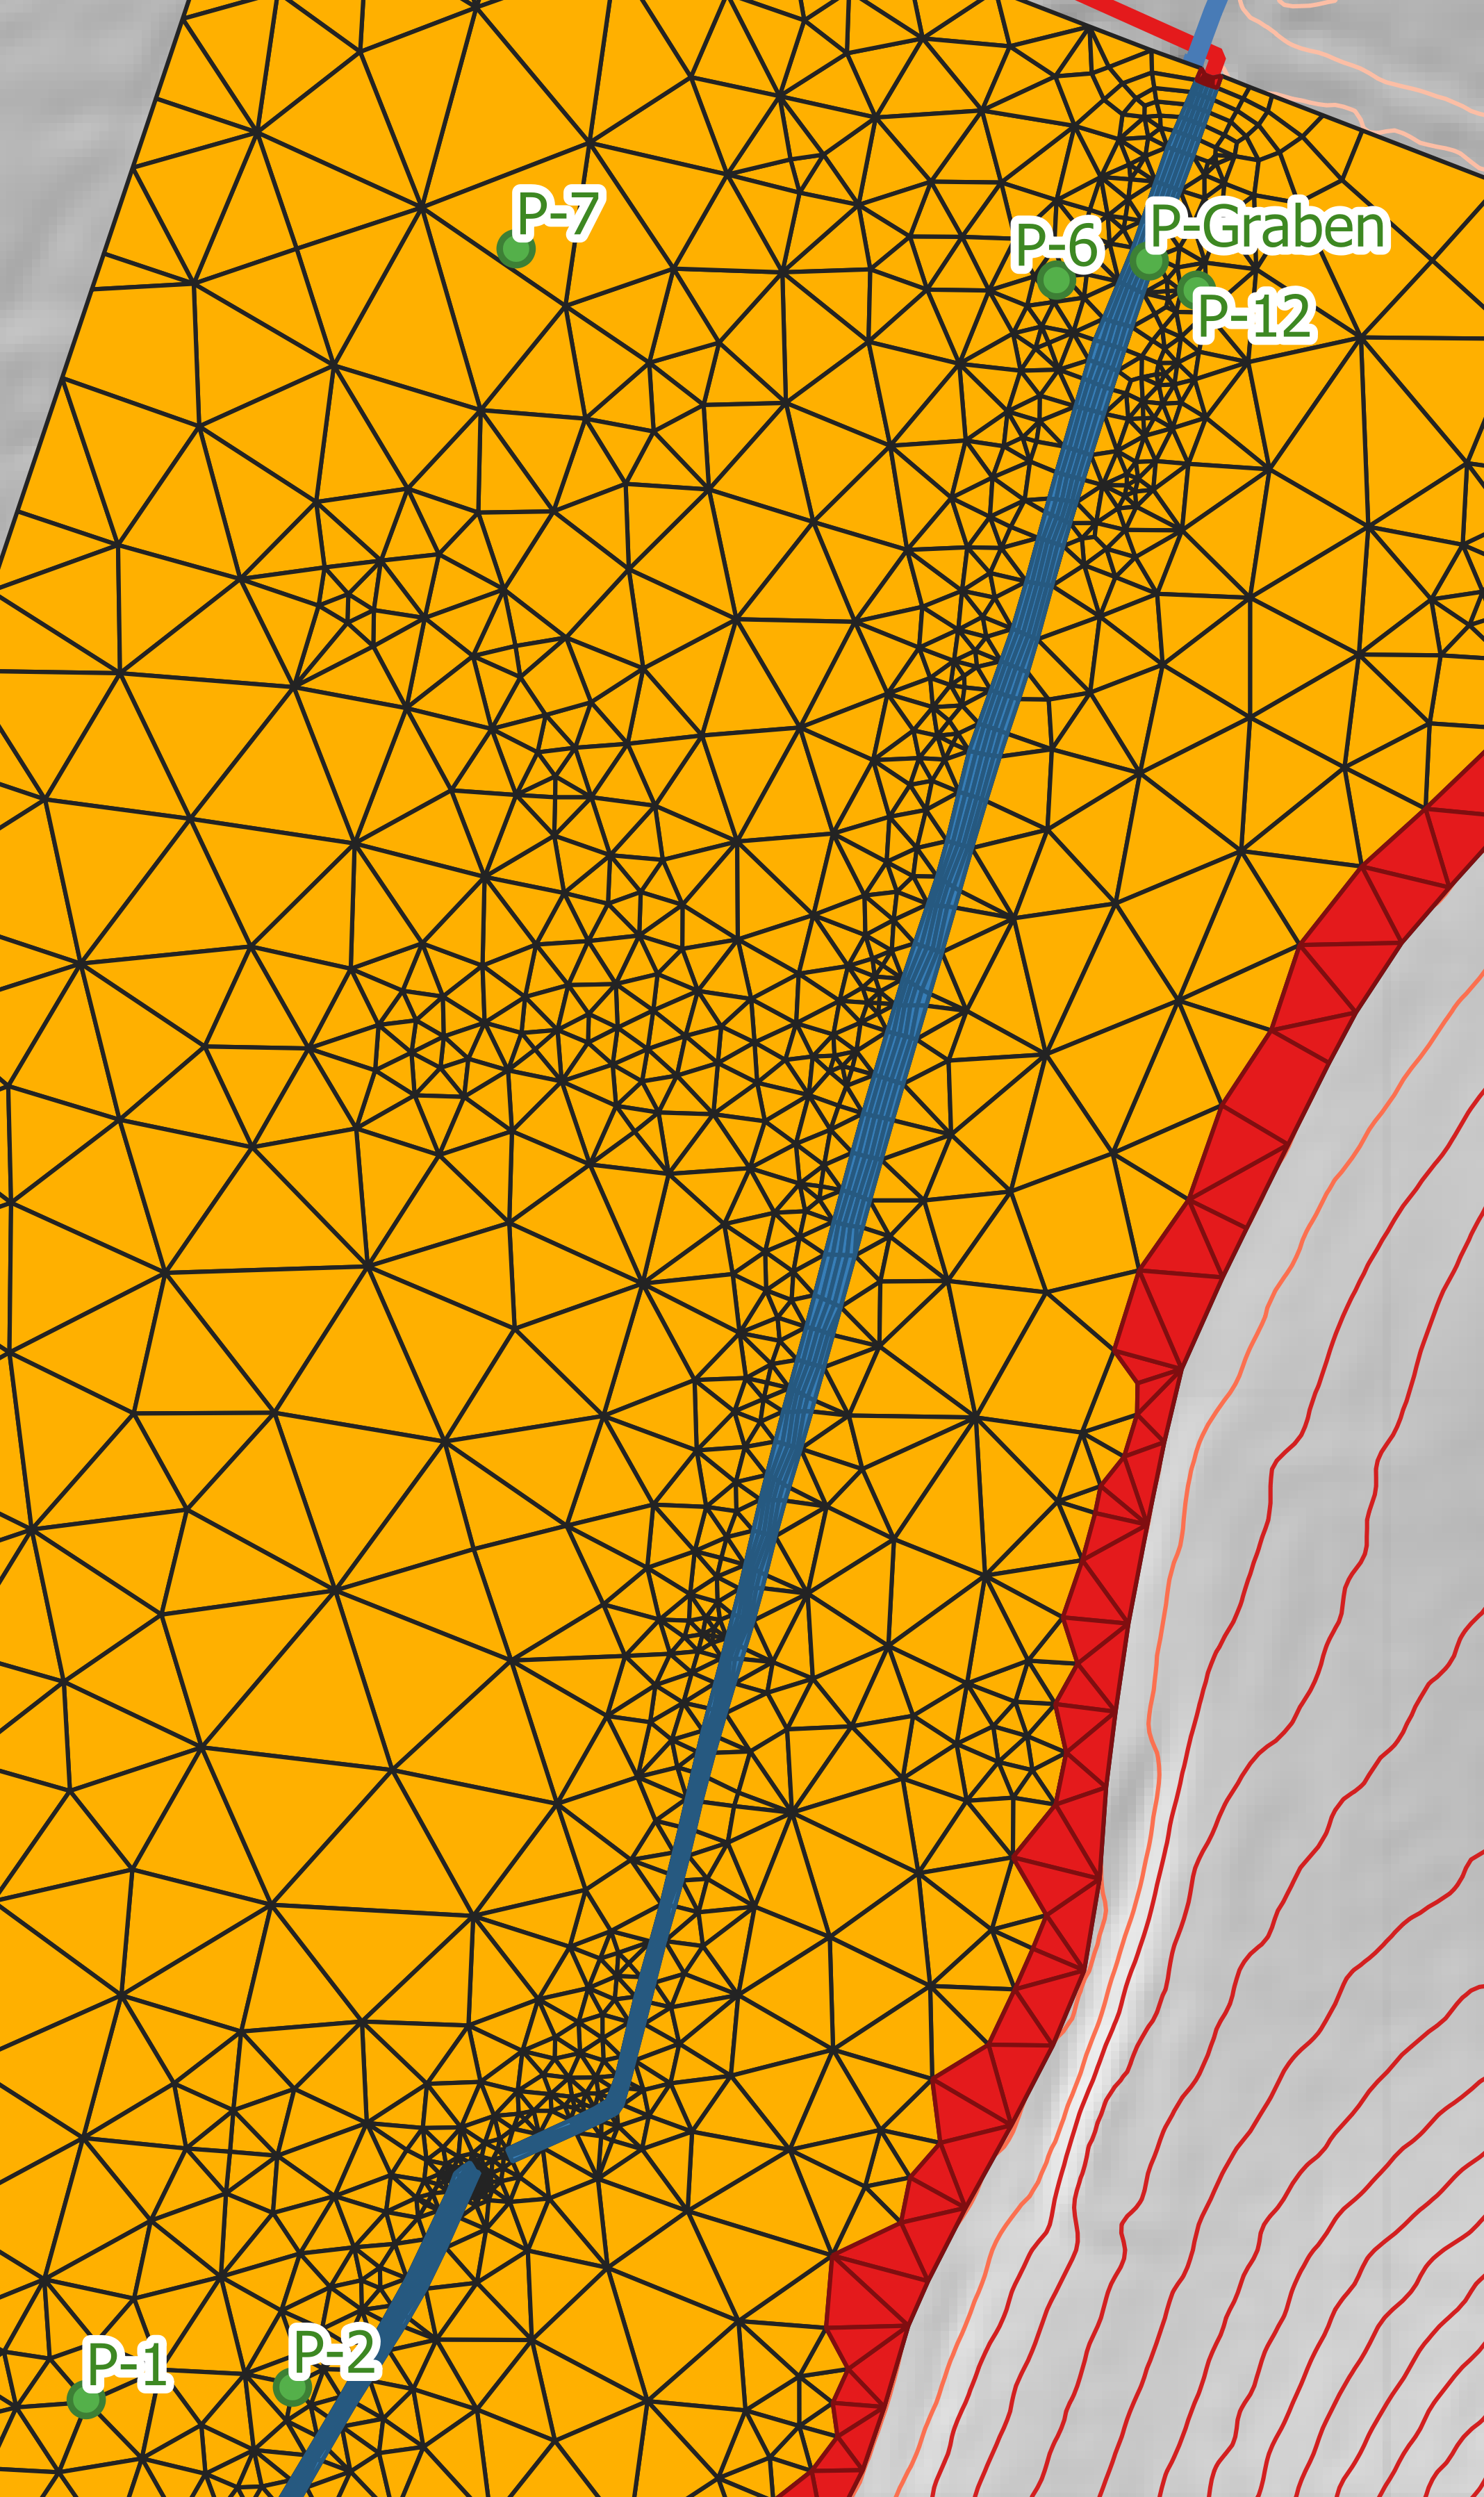
\includegraphics[height=\textheight]{PICTURES/models_ini/obs_pts.png}
    \caption{Locations of GW observation points.}
    \label{fig:obs_pts}
\end{figure}

\endinput
\chapter{Results and Discussion}
\label{results}
The simulation, set-up as defined in the previous chapter, was run on a regular PC with an Intel Core i5 (\nth{8} Generation) chipset, running on AC power.


\section{Runtimes}
The total runtime for the simulation period (1 month) was \unit[2187]{s} or \unit[36.45]{min}.
As seen in Figures \ref{fig:run_vs_p} and \ref{fig:runtimes}, the number of internal time steps and thus the local simulation runtimes increase with increasing precipitation intensities and vice versa, thus automatically increasing temporal resolution where necessary and avoiding excessive computations where it is not necessary.
\begin{figure}[H]
    \centering
    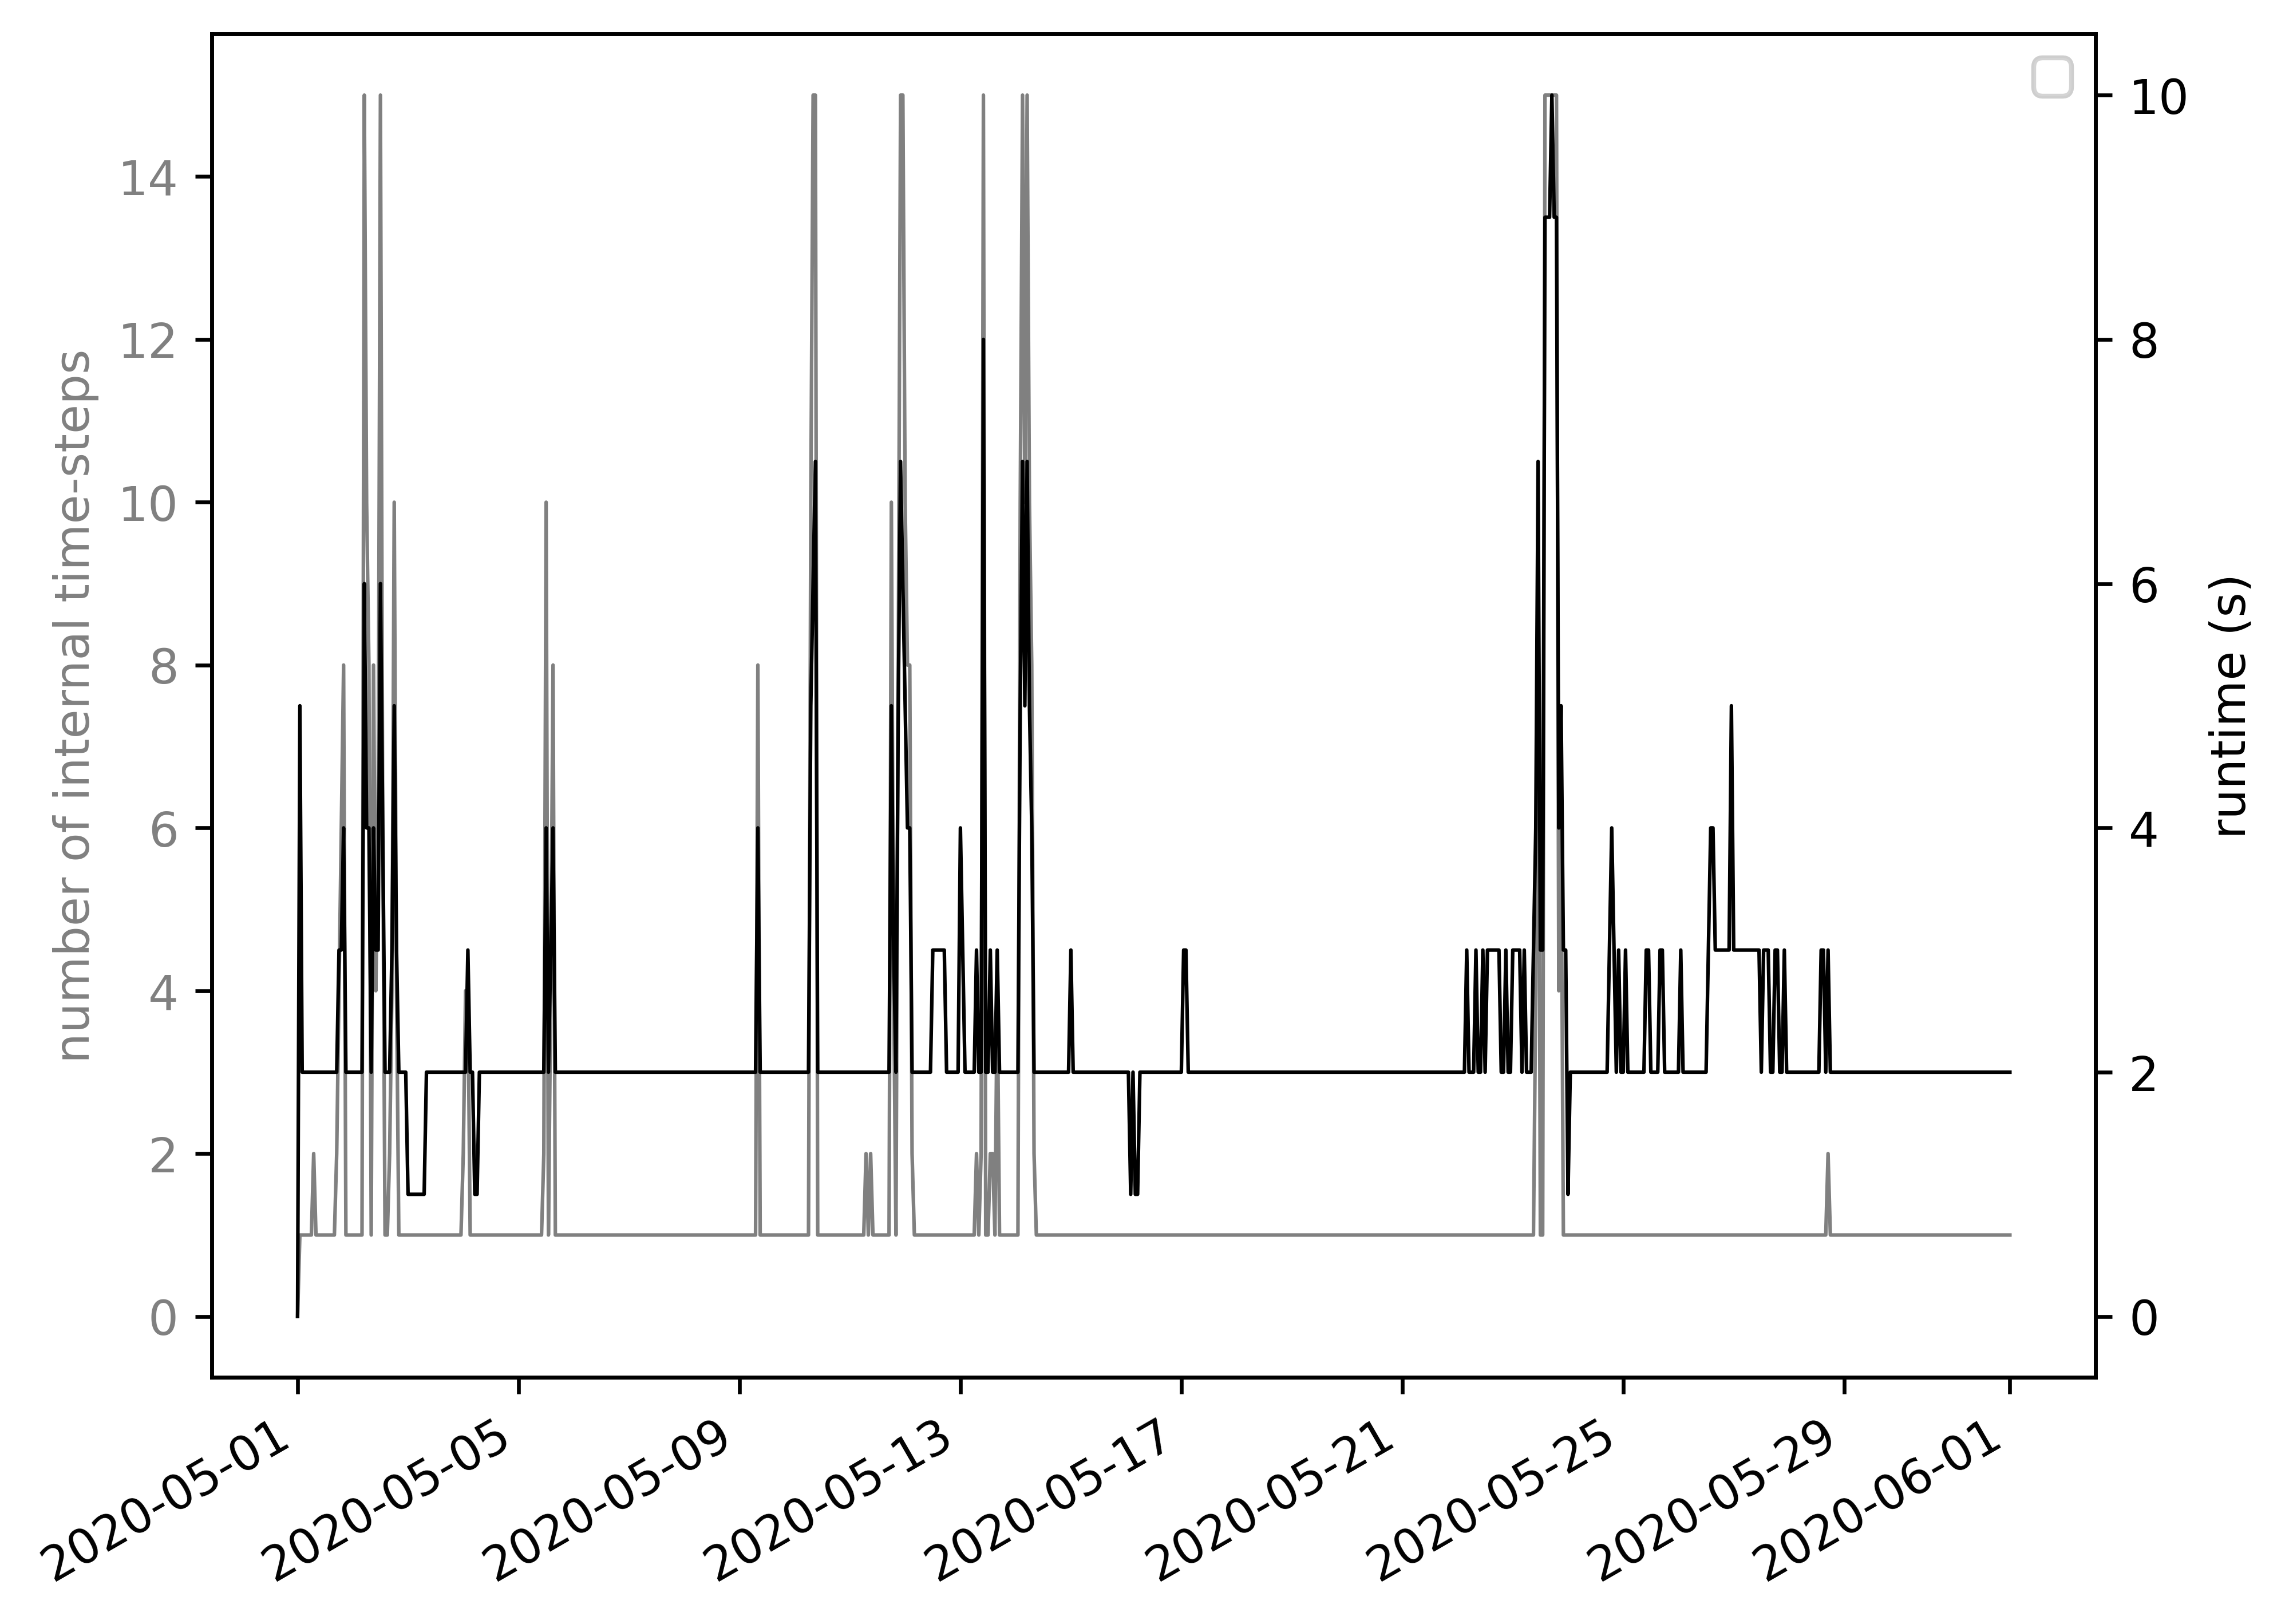
\includegraphics[width=\linewidth]{PICTURES/models_res/runtimes}
    \caption{Runtimes (s) and number of time-steps per local simulation period over the global simulation period.}
    \label{fig:runtimes}
\end{figure}
\begin{figure}[H]
    \centering
    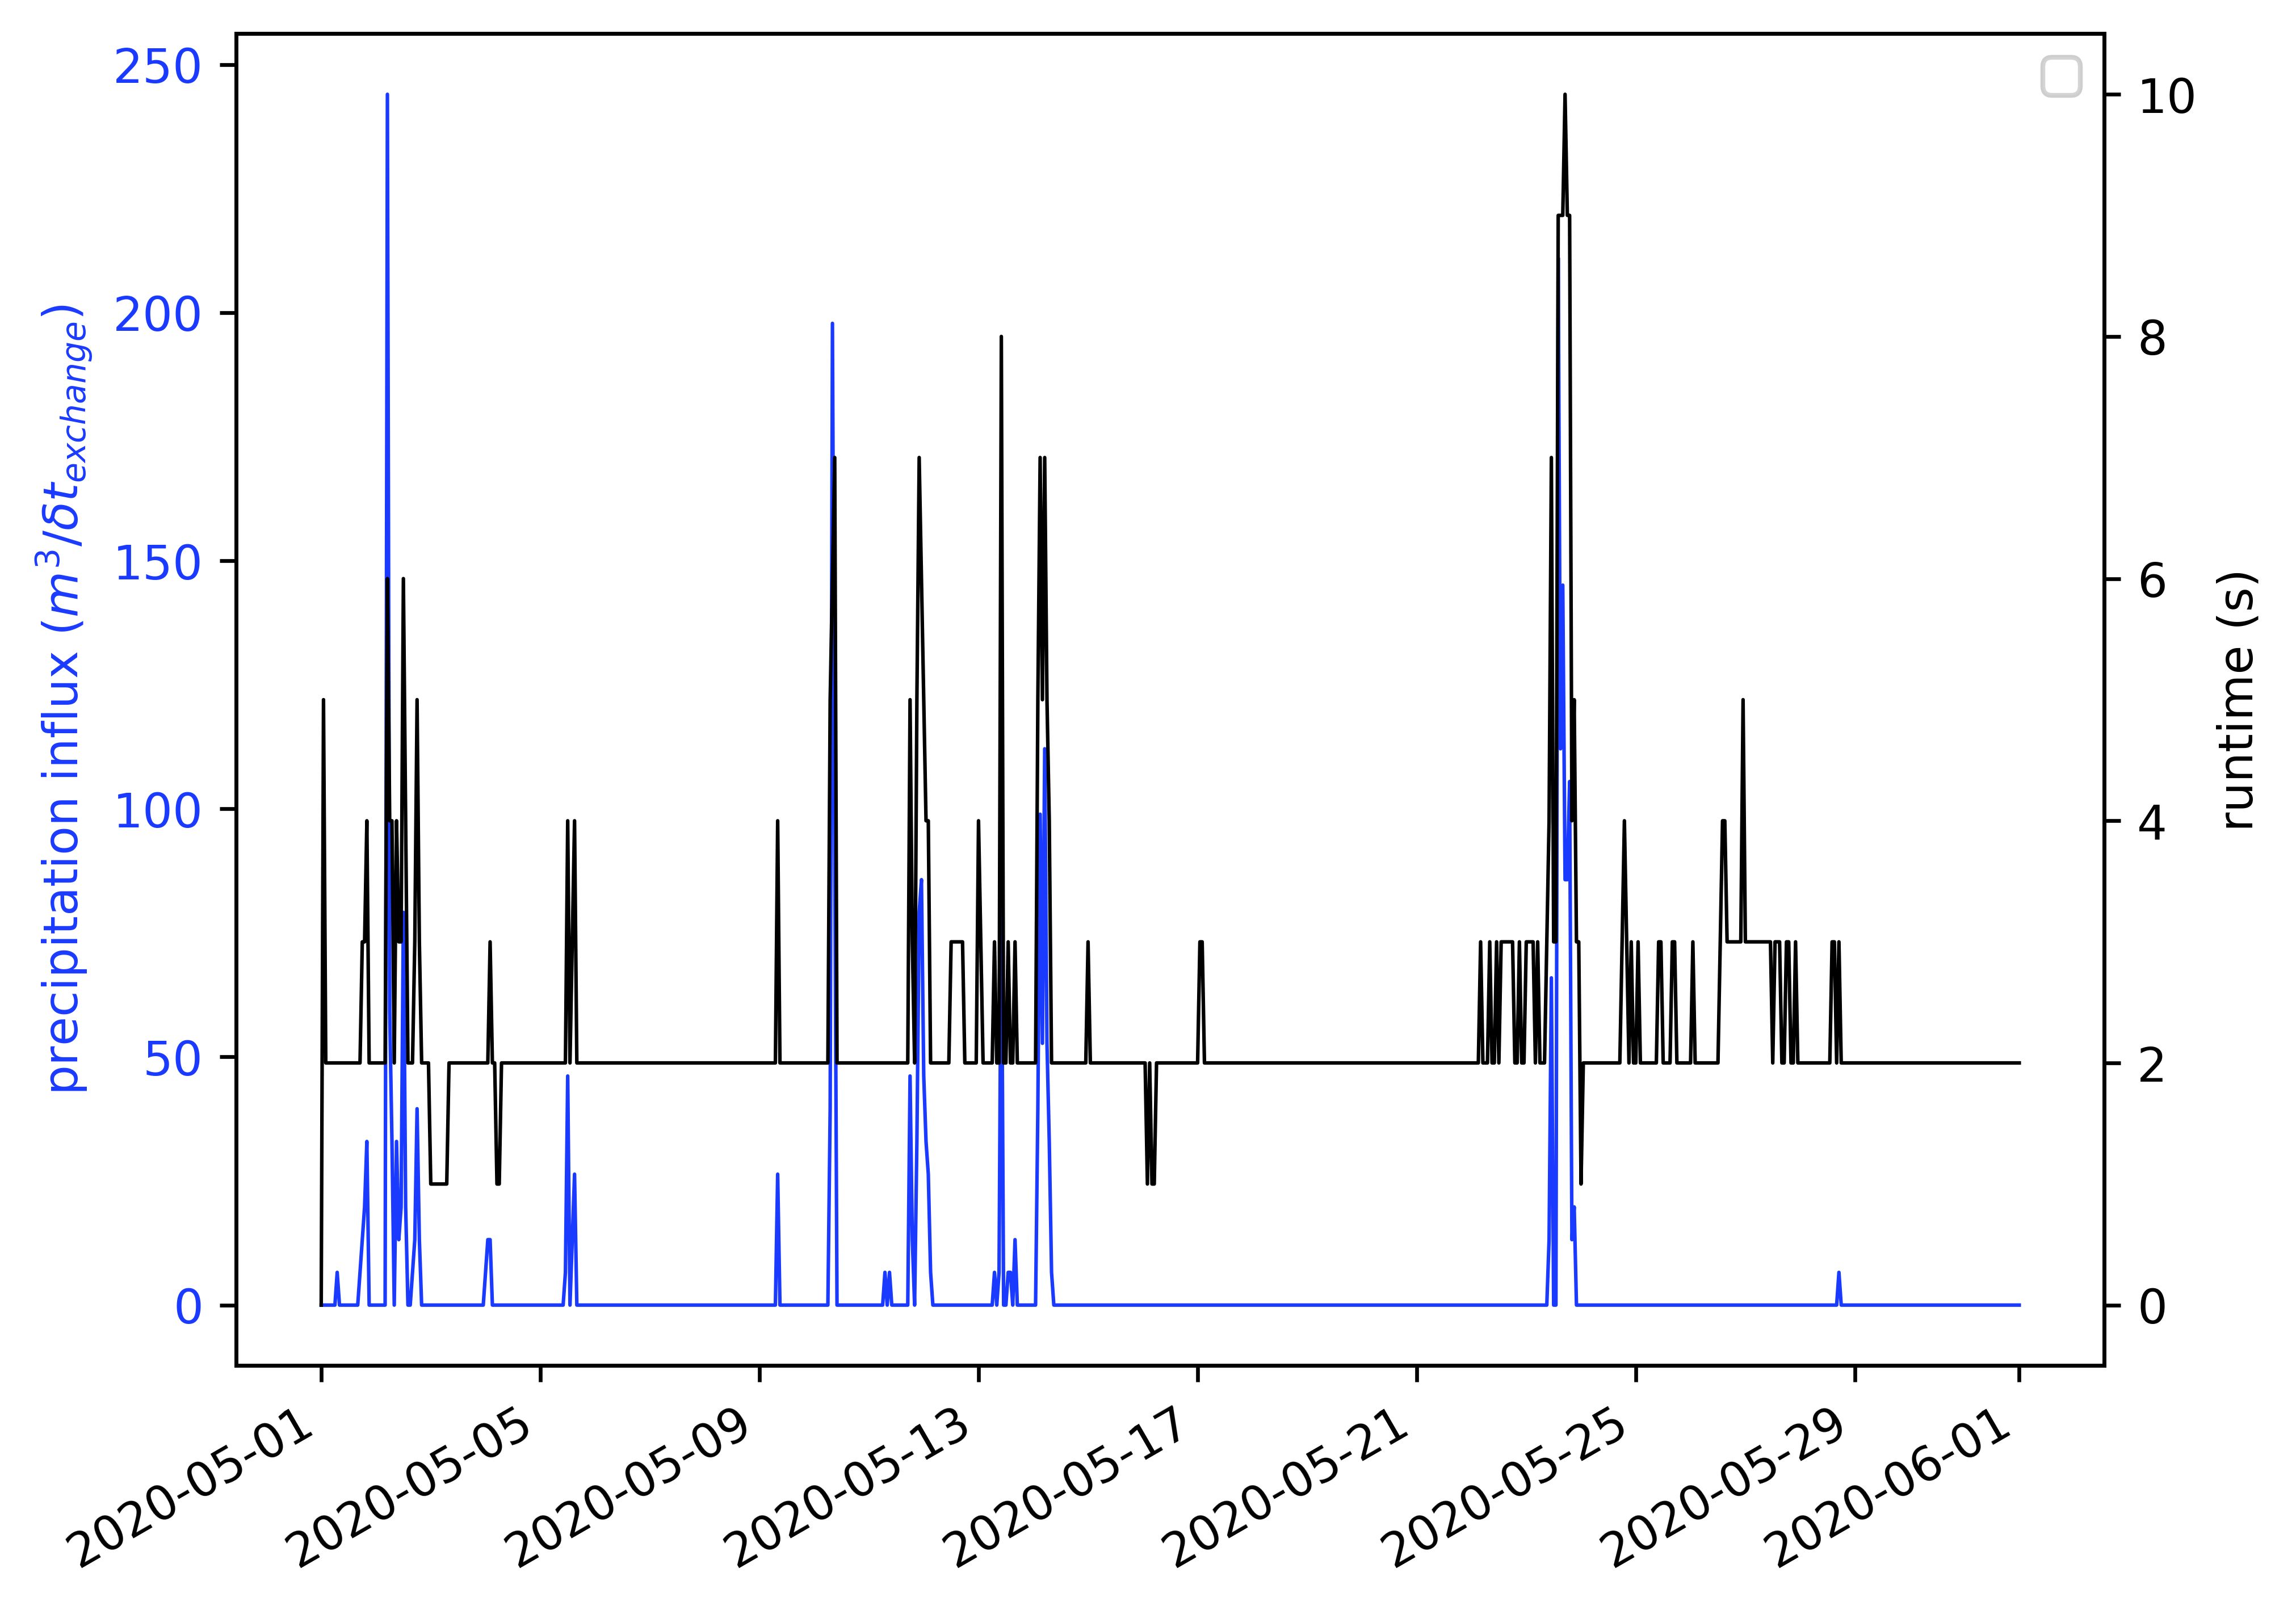
\includegraphics[width=\linewidth]{PICTURES/models_res/run_vs_p}
    \caption{Correlating precipitation intensities with Runtimes (s).}
    \label{fig:run_vs_p}
\end{figure}


\section{Mass Balance}
\label{mass_balance}
Figure \ref{fig:mass_balance_total} illustrates the mass balance of the GWSWEX model and the coupling scheme. It is safe to say that a good mass balance is achieved. The mass balance is calculated for each local simulation period as follows:
\begin{gather}
    \nonumber Q_{in} = P - ET \\
    \nonumber Q_{out} = SM_{dis} + GW_{dis} + SW_{dis}
\end{gather}

where
\begin{tabbing}
    $P$ \hspace{.4in}\= = precipitation influx in $m^3$,\\
    $ET$ \>= evapotranspiration outflux in $m^3$, \\ 
    $SM_{dis}$ \>= discharges in the SM storage term in $m^3$,\\
    $GW_{dis}$ \>= discharges in the GW storage term in $m^3$, and\\
    $SW_{dis}$ \>= discharges in the SW storage term in $m^3$.\\
\end{tabbing}


As seen in table \ref{tab:results} and the subsequent figures, the evapotranspiration outflux, owing to its volume, and precipitation influx follows it. \\

\begin{table}[H]
\caption{Consolidated summary of the simulation results}
\label{tab:results}
\centering
\begin{tabular}{lr}
\hline\noalign{\smallskip}
quantity & flux (in: +ve, out: -ve)  \\
\noalign{\smallskip}\hline\noalign{\smallskip}
evapotranspiration  & \SI{-5654.71}{\cubic\metre} \\
precipitation  & +\SI{2901.39}{\cubic\metre} \\
\hline\noalign{\smallskip}
IN, GWSWEX & \SI{-2753.32}{\cubic\metre} \\
\hline\noalign{\smallskip}
SM discharge & \SI{-3892.95}{\cubic\metre} \\
GW discharge & +\SI{1117.94}{\cubic\metre} \\
SW discharge & +\SI{7.51}{\cubic\metre} \\
\hline\noalign{\smallskip}
OUT, GWSWEX & \SI{-2767.52}{\cubic\metre} \\
\noalign{\smallskip}\hline
Error & \SI{-14.19}{\cubic\metre} (0.51\%) \\
\noalign{\smallskip}\hline
\end{tabular}
\end{table}

\subsection{Addressing the Discrepancy}
\begin{figure}[H]
    \centering
    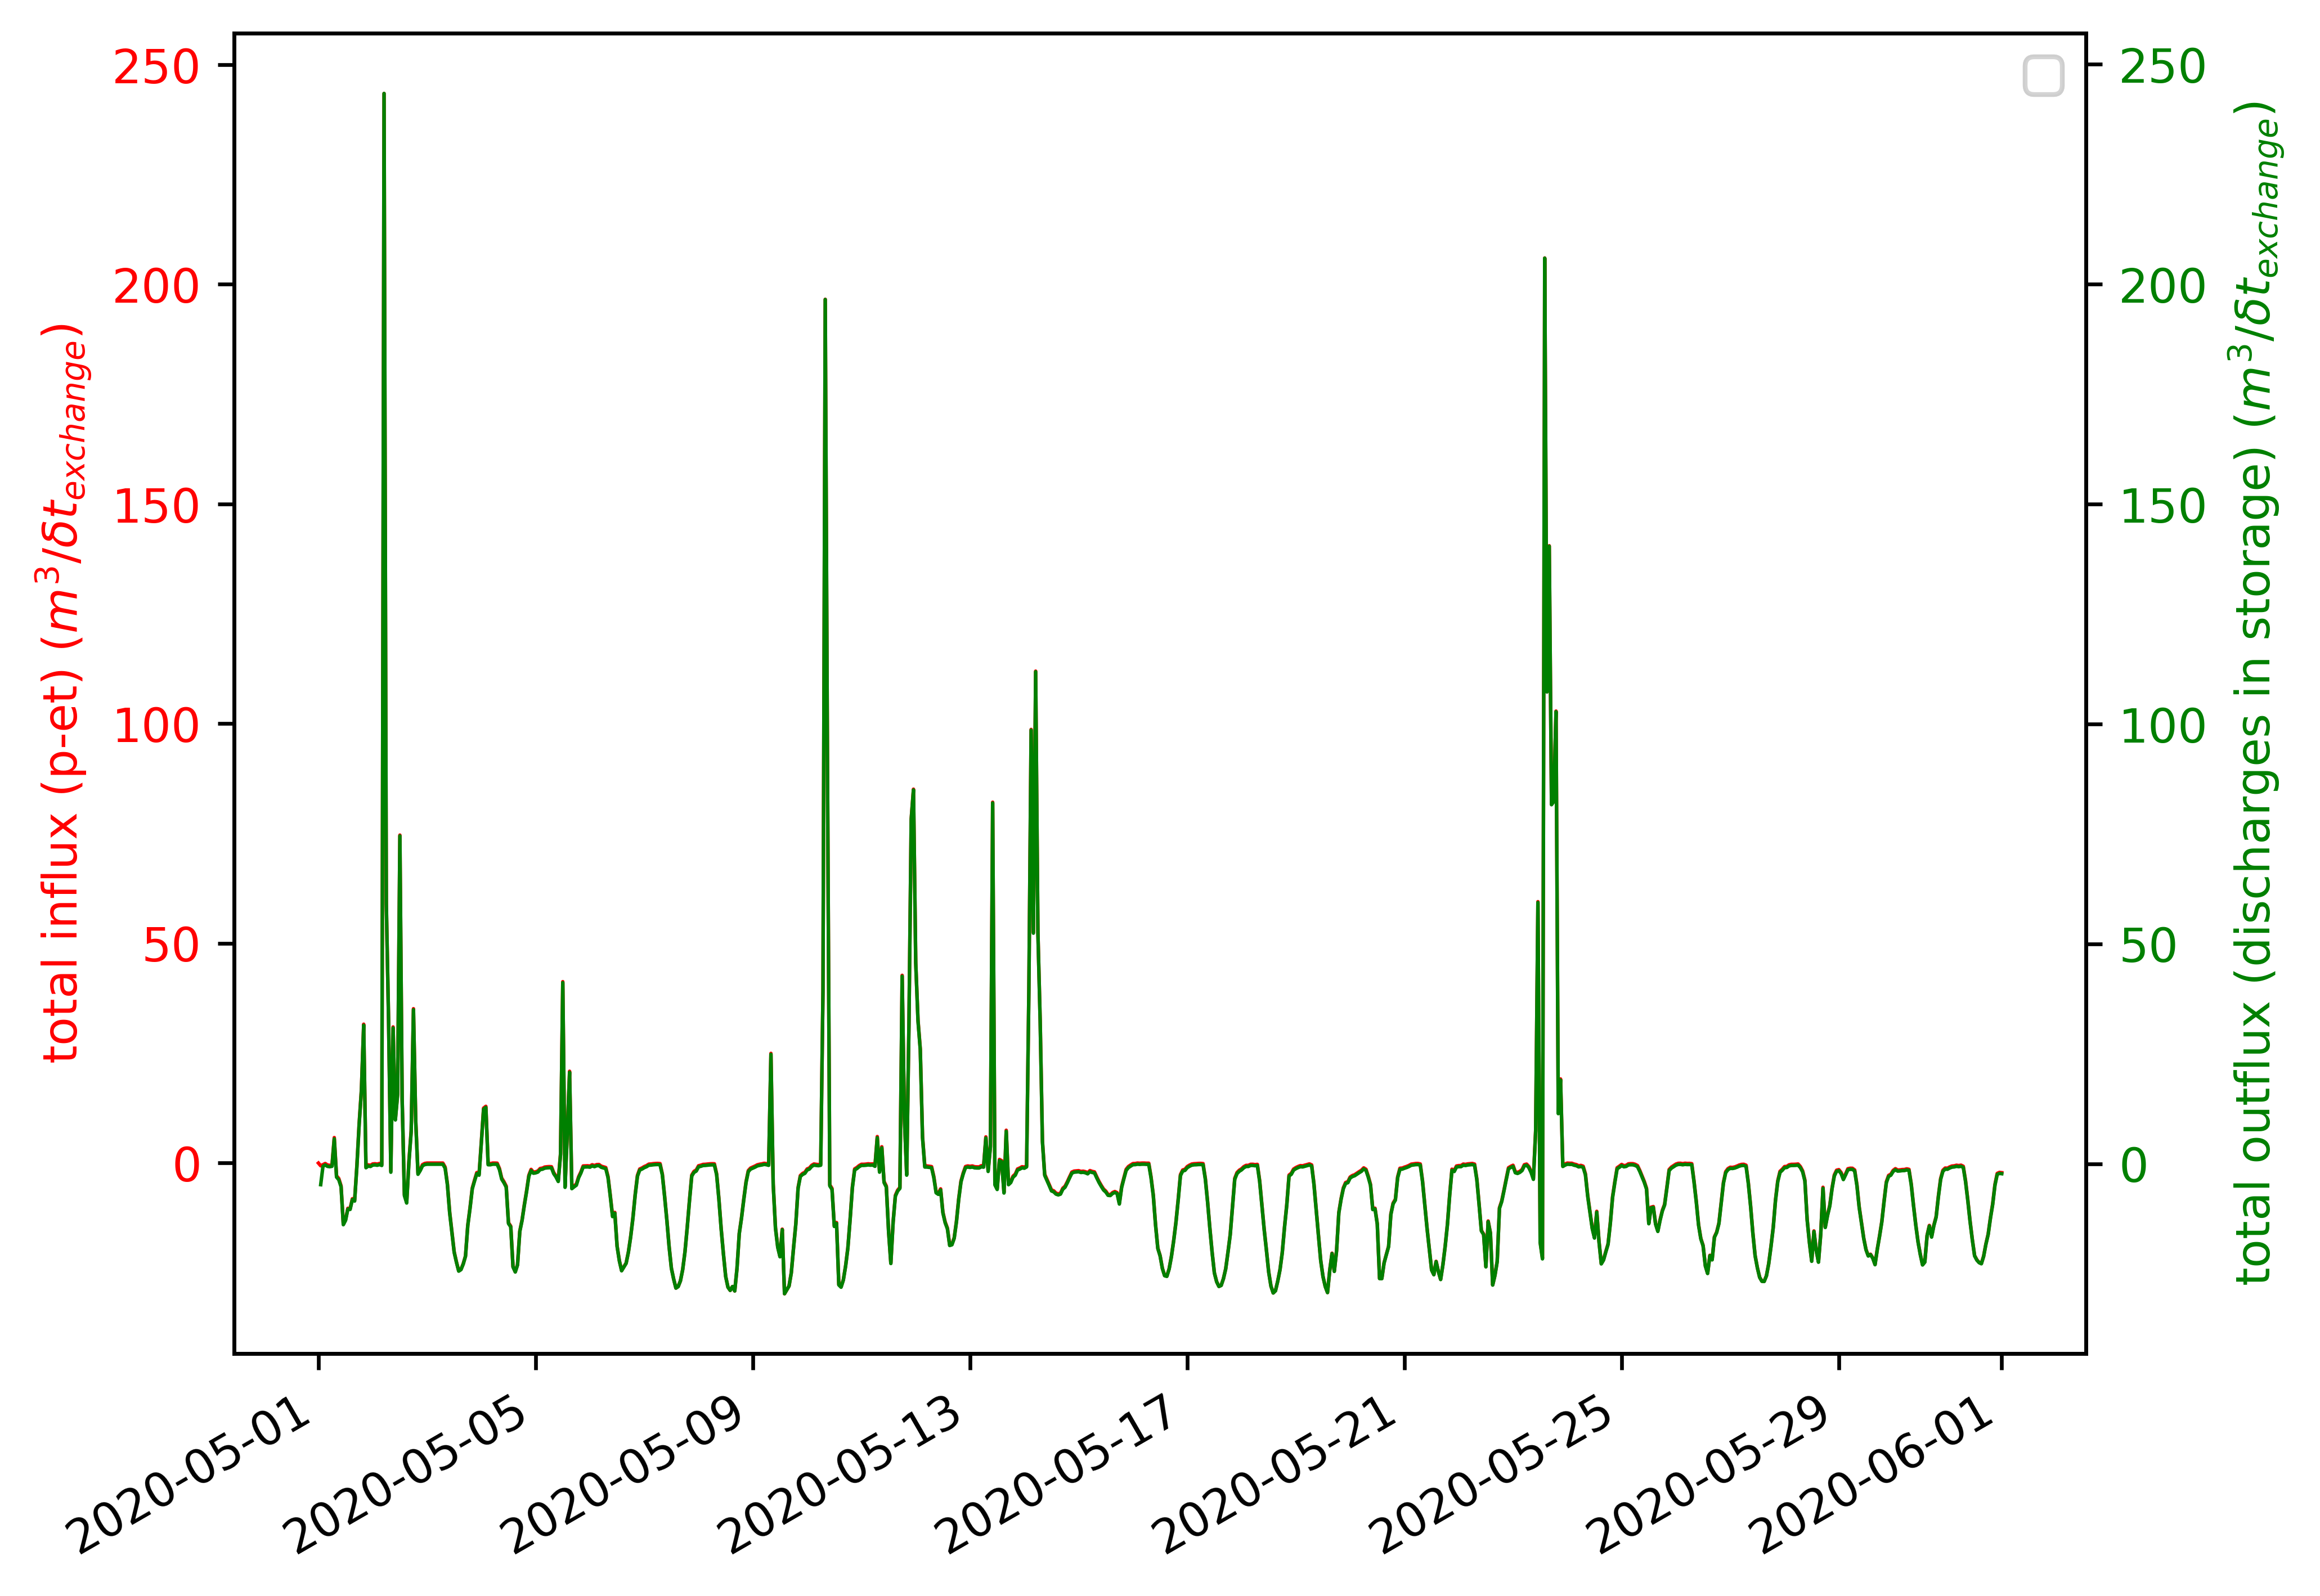
\includegraphics[width=\linewidth]{PICTURES/models_res/mass_balance}
    \caption{Mass balance.}
    \label{fig:mass_balance_total}
\end{figure}

The mass balance discrepancy can be attributed to a known flaw in the coupling scheme/SW model. It is documented that D-Flow FM relaxes negative lateral discharges with a factor of 0.5 when the storage is deemed \textit{inadequate}. However, it is not clearly defined what amount of storage is adequate to avoid relaxation of negative discharges. Figure \ref{fig:err_delft-fort} illustrates this discrepancy over the simulation period.
\begin{figure}[H]
    \centering
    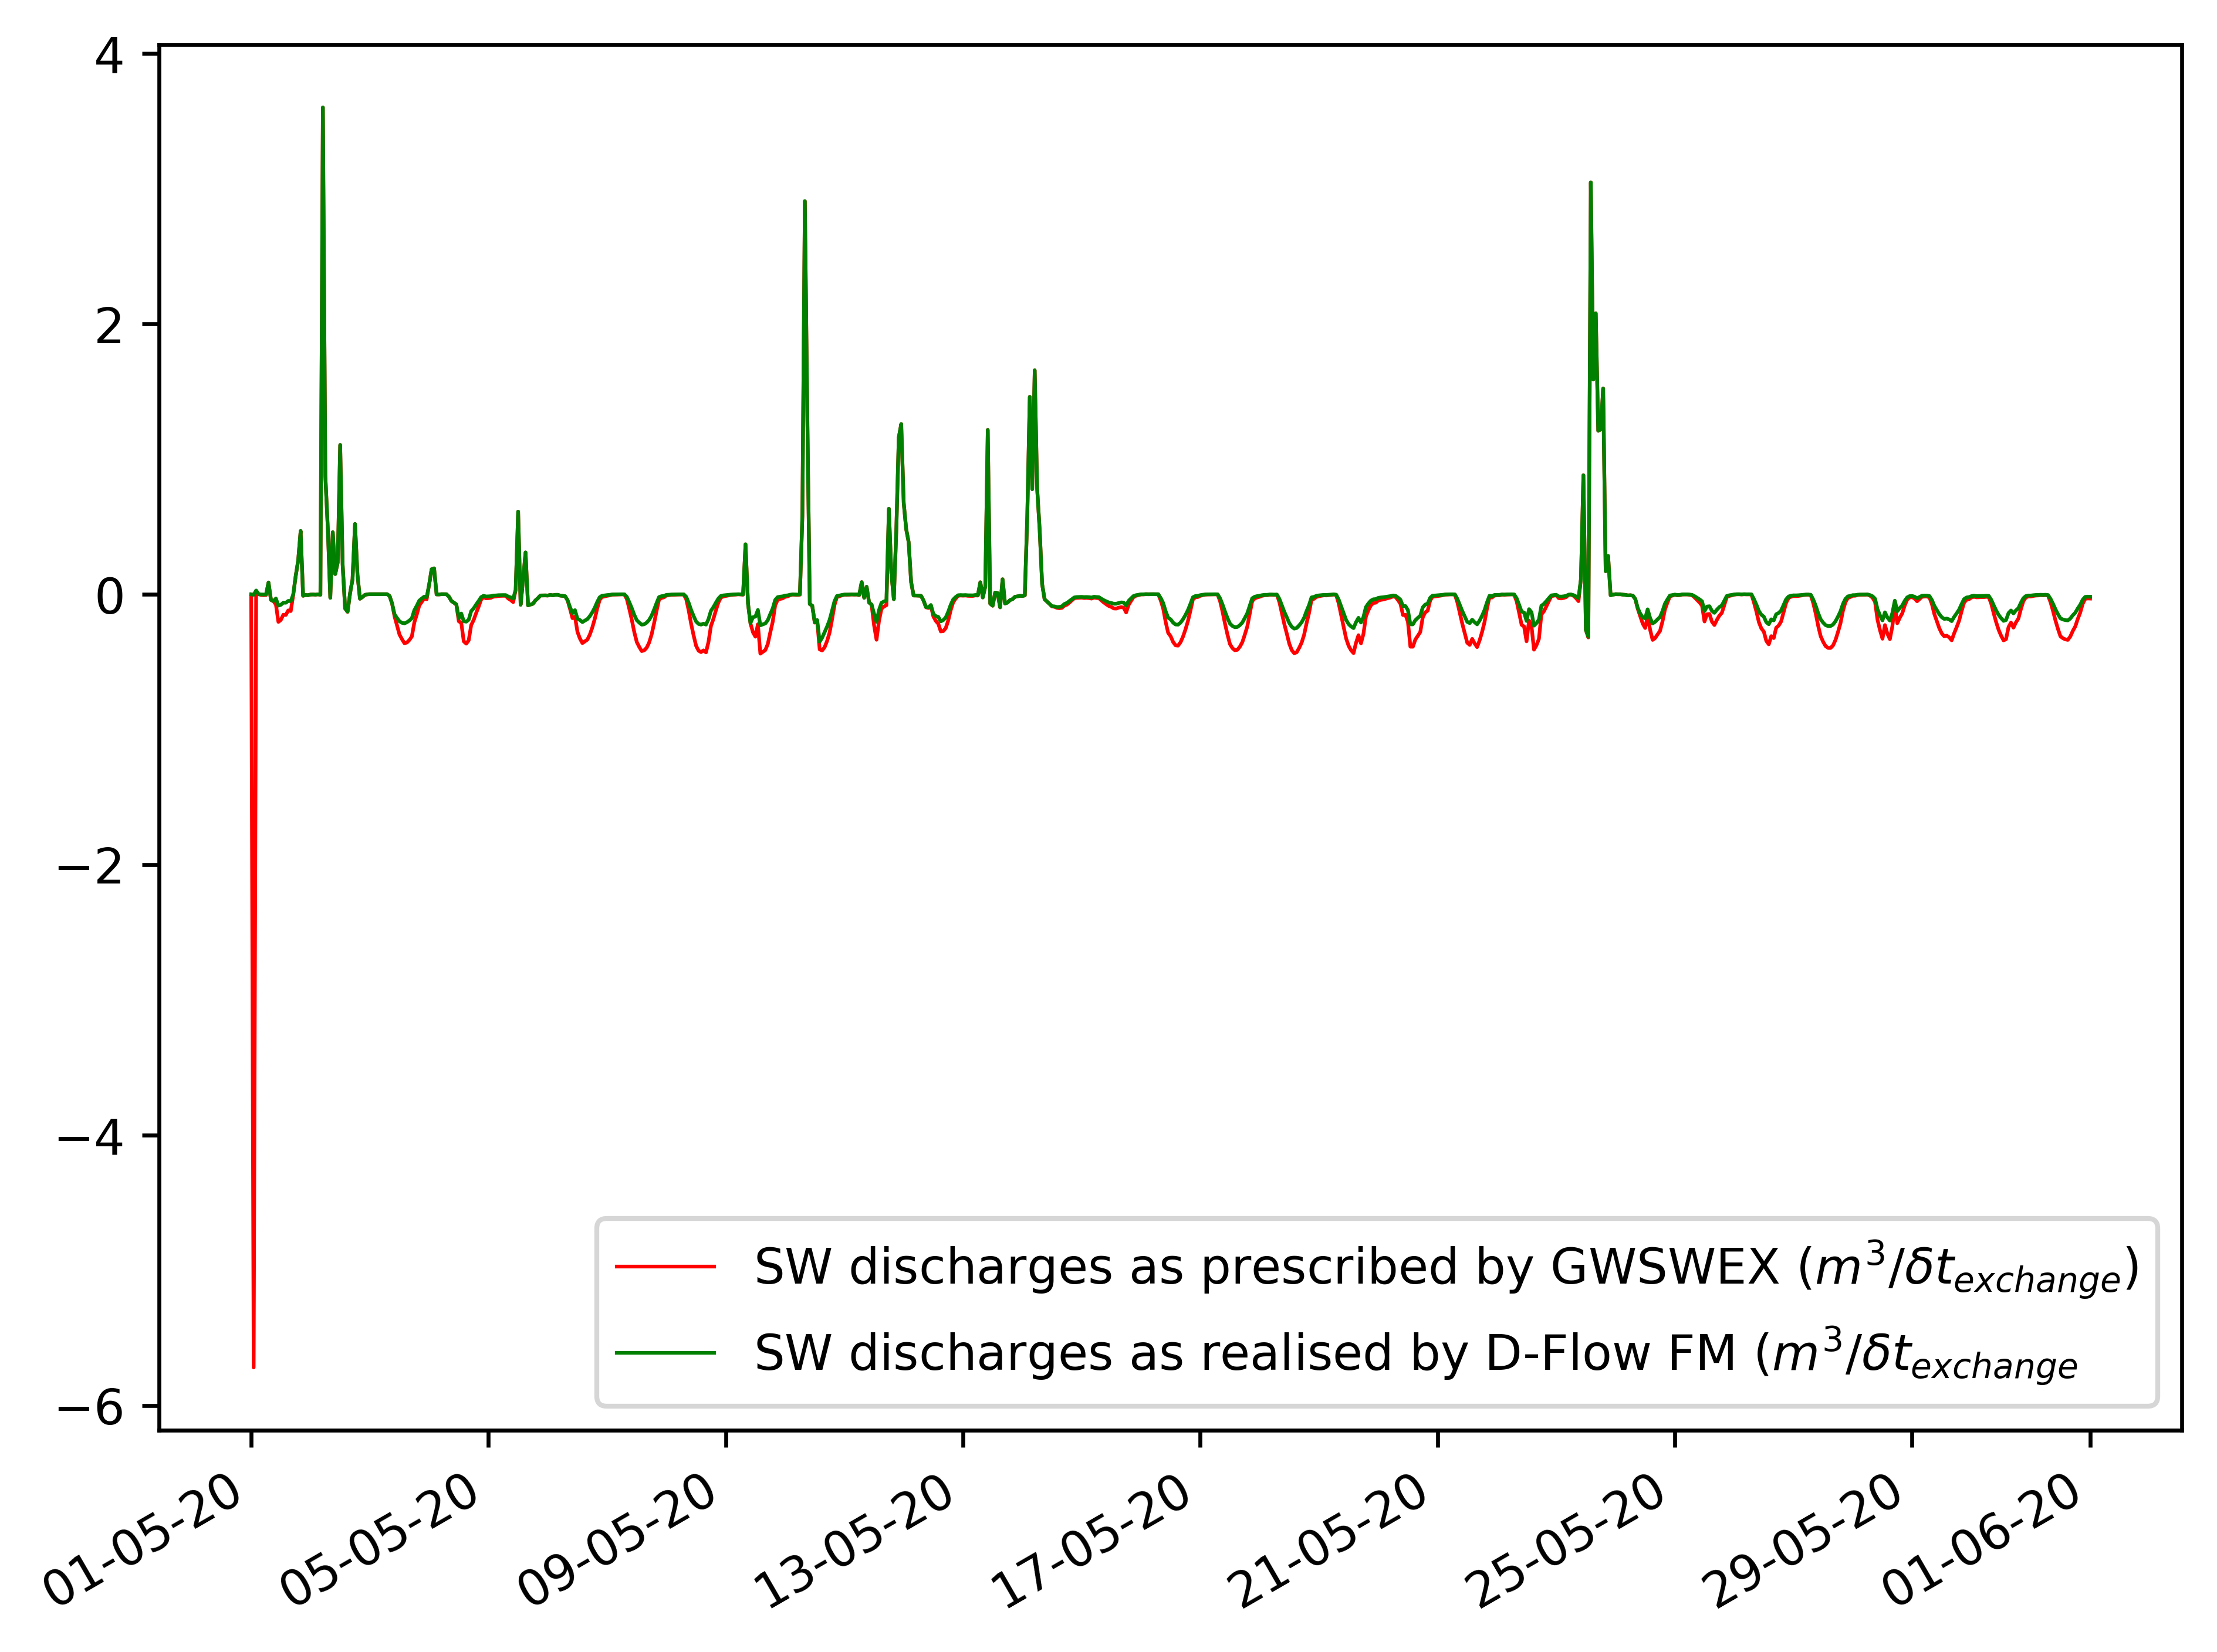
\includegraphics[width=\linewidth]{PICTURES/models_res/err_delft-fort}
    \caption{Discrepancy between prescribed and realised SW storage discharges.}
    \label{fig:err_delft-fort}
\end{figure}

The residual error in the GWSWEX model, as seen in Figure \ref{fig:err_fort} is rather negligible.
\begin{figure}[H]
    \centering
    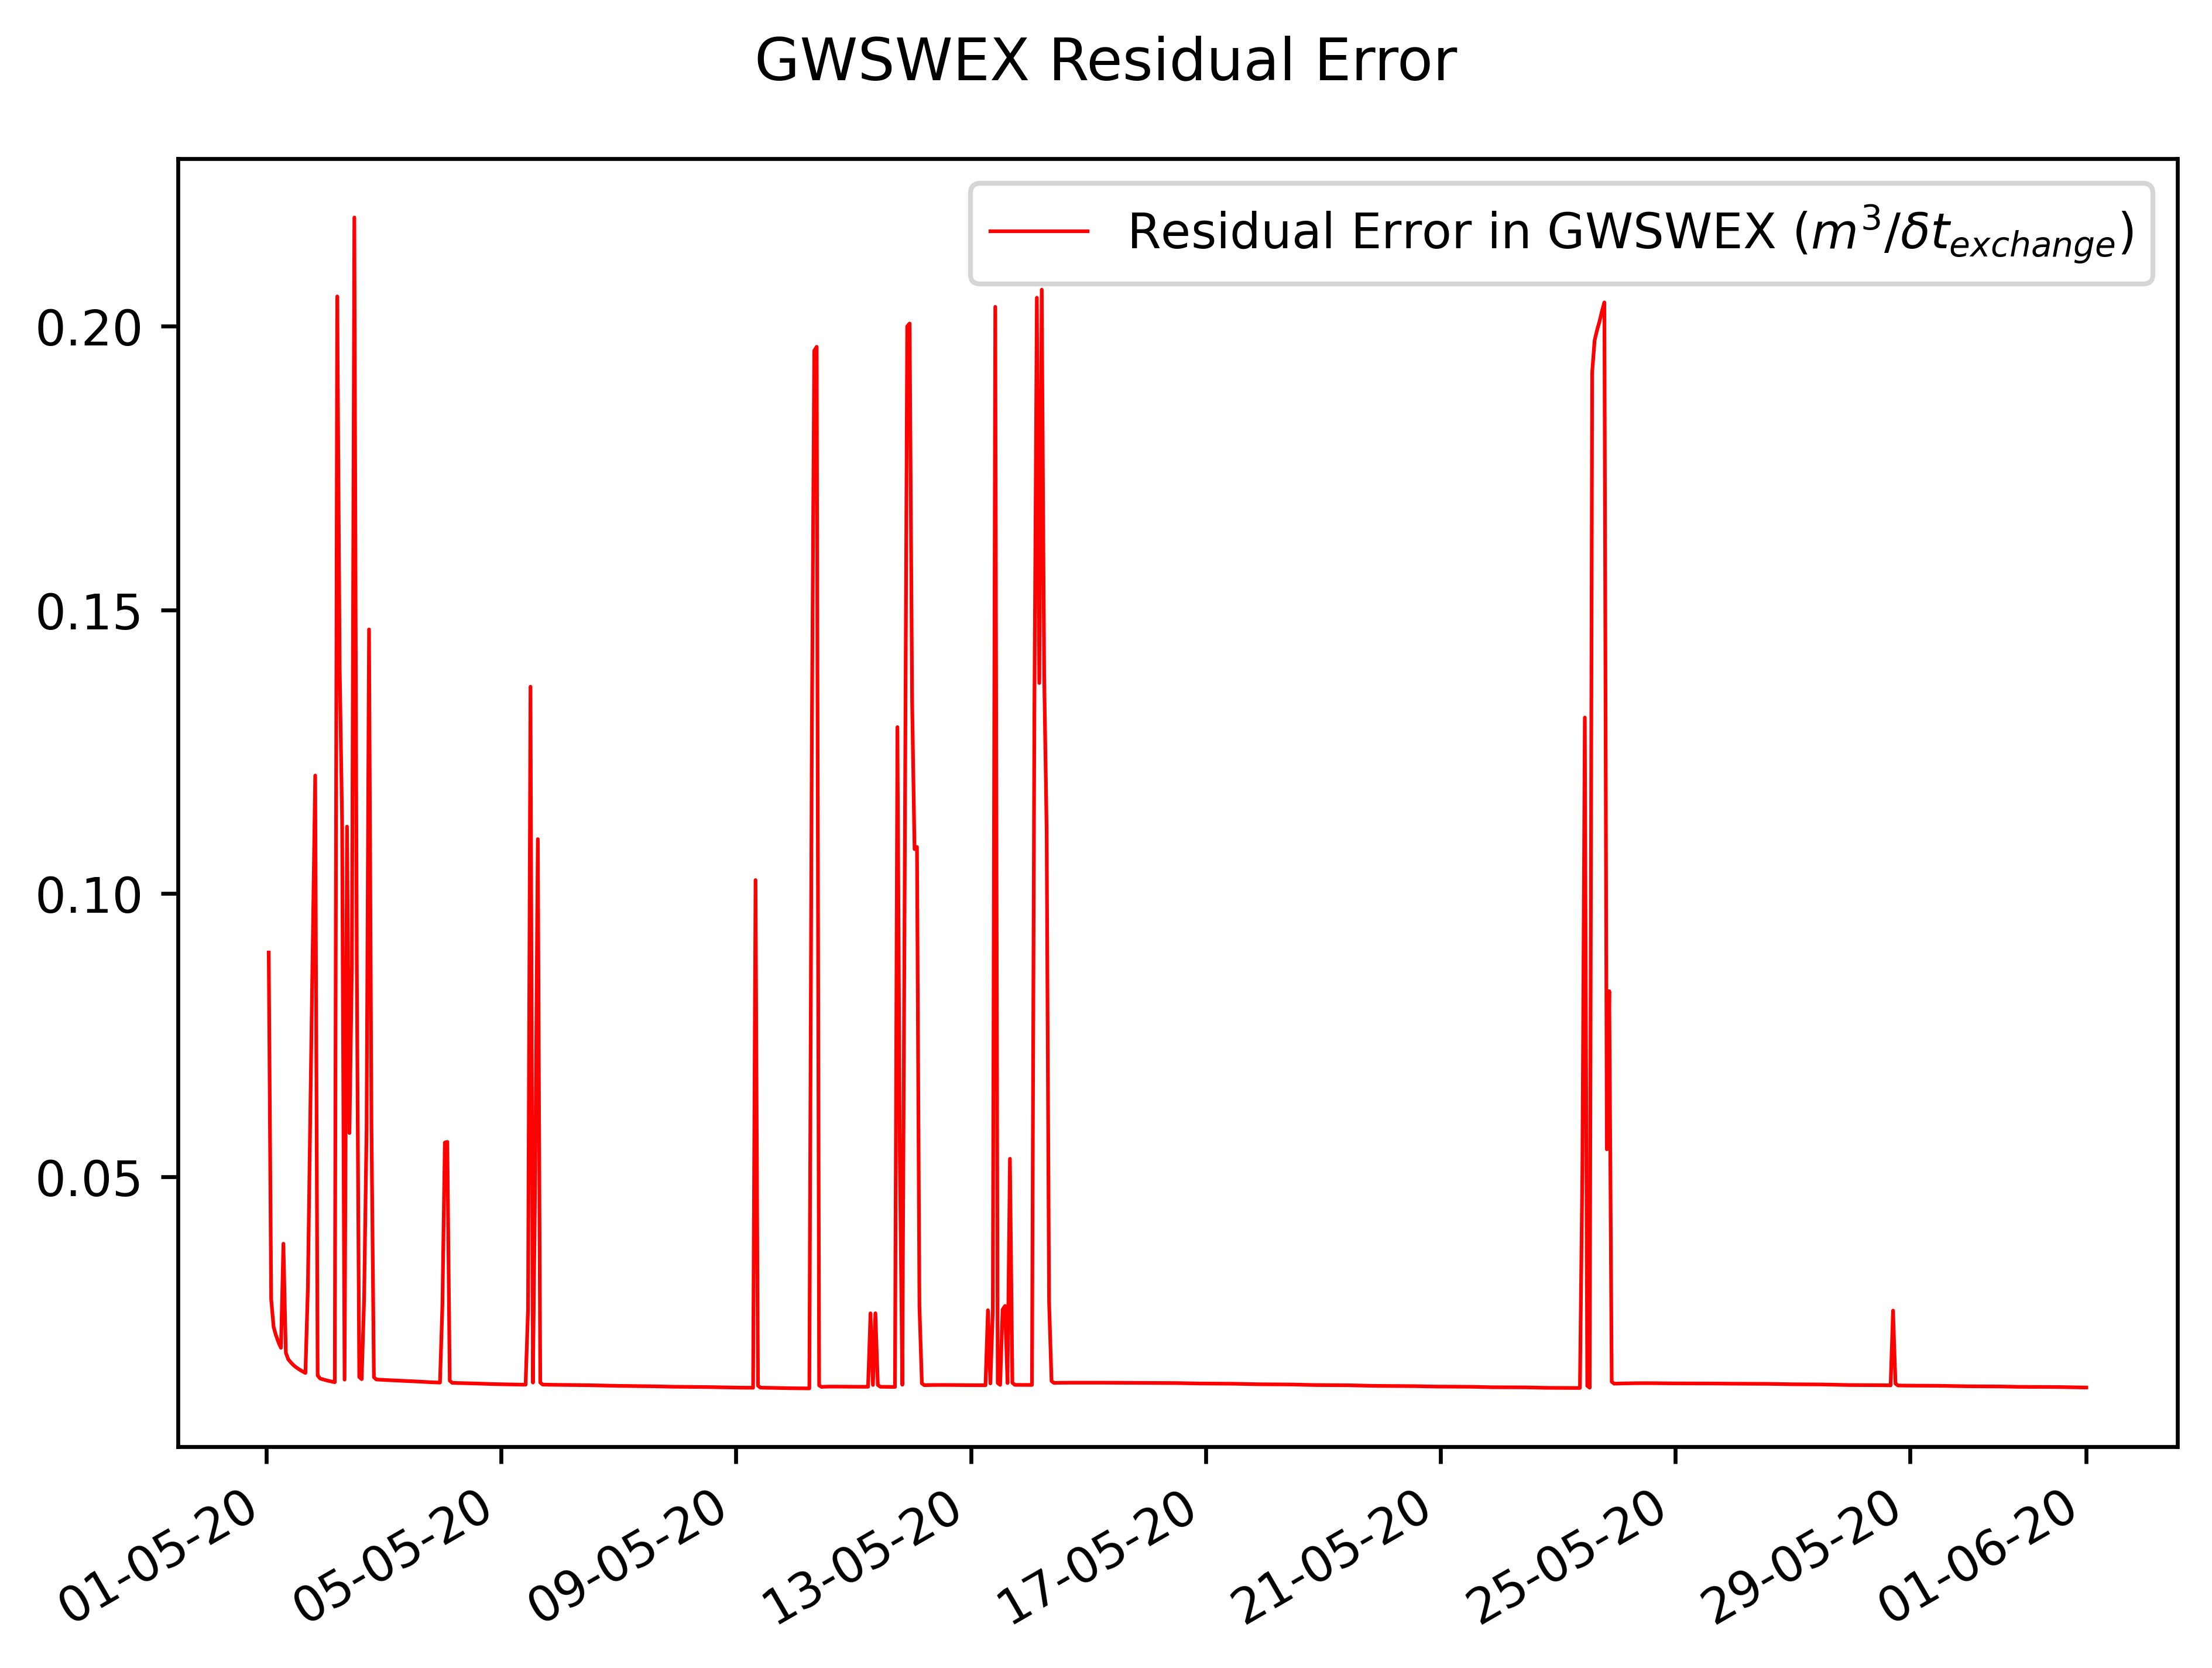
\includegraphics[width=\linewidth]{PICTURES/models_res/err_fort}
    \caption{Residual error in the GWSWEX model.}
    \label{fig:err_fort}
\end{figure}

\subsection{Following Evapotranspiration Outflux}
The following plots compare the ET outflux to the discharges in the three storages in an effort to both elucidate the behaviour of the model and to assess if the outcome is as one might expect.
\\ \\
As observed from Figures \ref{fig:et_vs_sm} and \ref{fig:et_vs_gw}, most of the ET outflux is satisfied by reduction in SM storage, especially until 26-05-2020, following which contribution from GW storage towards satisfying the ET outflux increases. This shift may have occurred as SM storage of a good portion of the model area, especially around the dewatering stream, has been reduced to $SM_\textrm{min}$ as seen in Figure \ref{fig:sm_res}. Increasing the GWSWEX model parameter, $m$, shall bring about this shift quicker and vice versa. One can observe, here, the consequence of this model parameter that defines the irreducible part of the SM storage - $SM_\textrm{min}$.
\\ \\
As was expected, contribution from the SW storage was negligible towards satisfying the ET outfluxes, as seen in Figure \ref{fig:et_vs_sw}.


\begin{figure}[H]
    \centering
    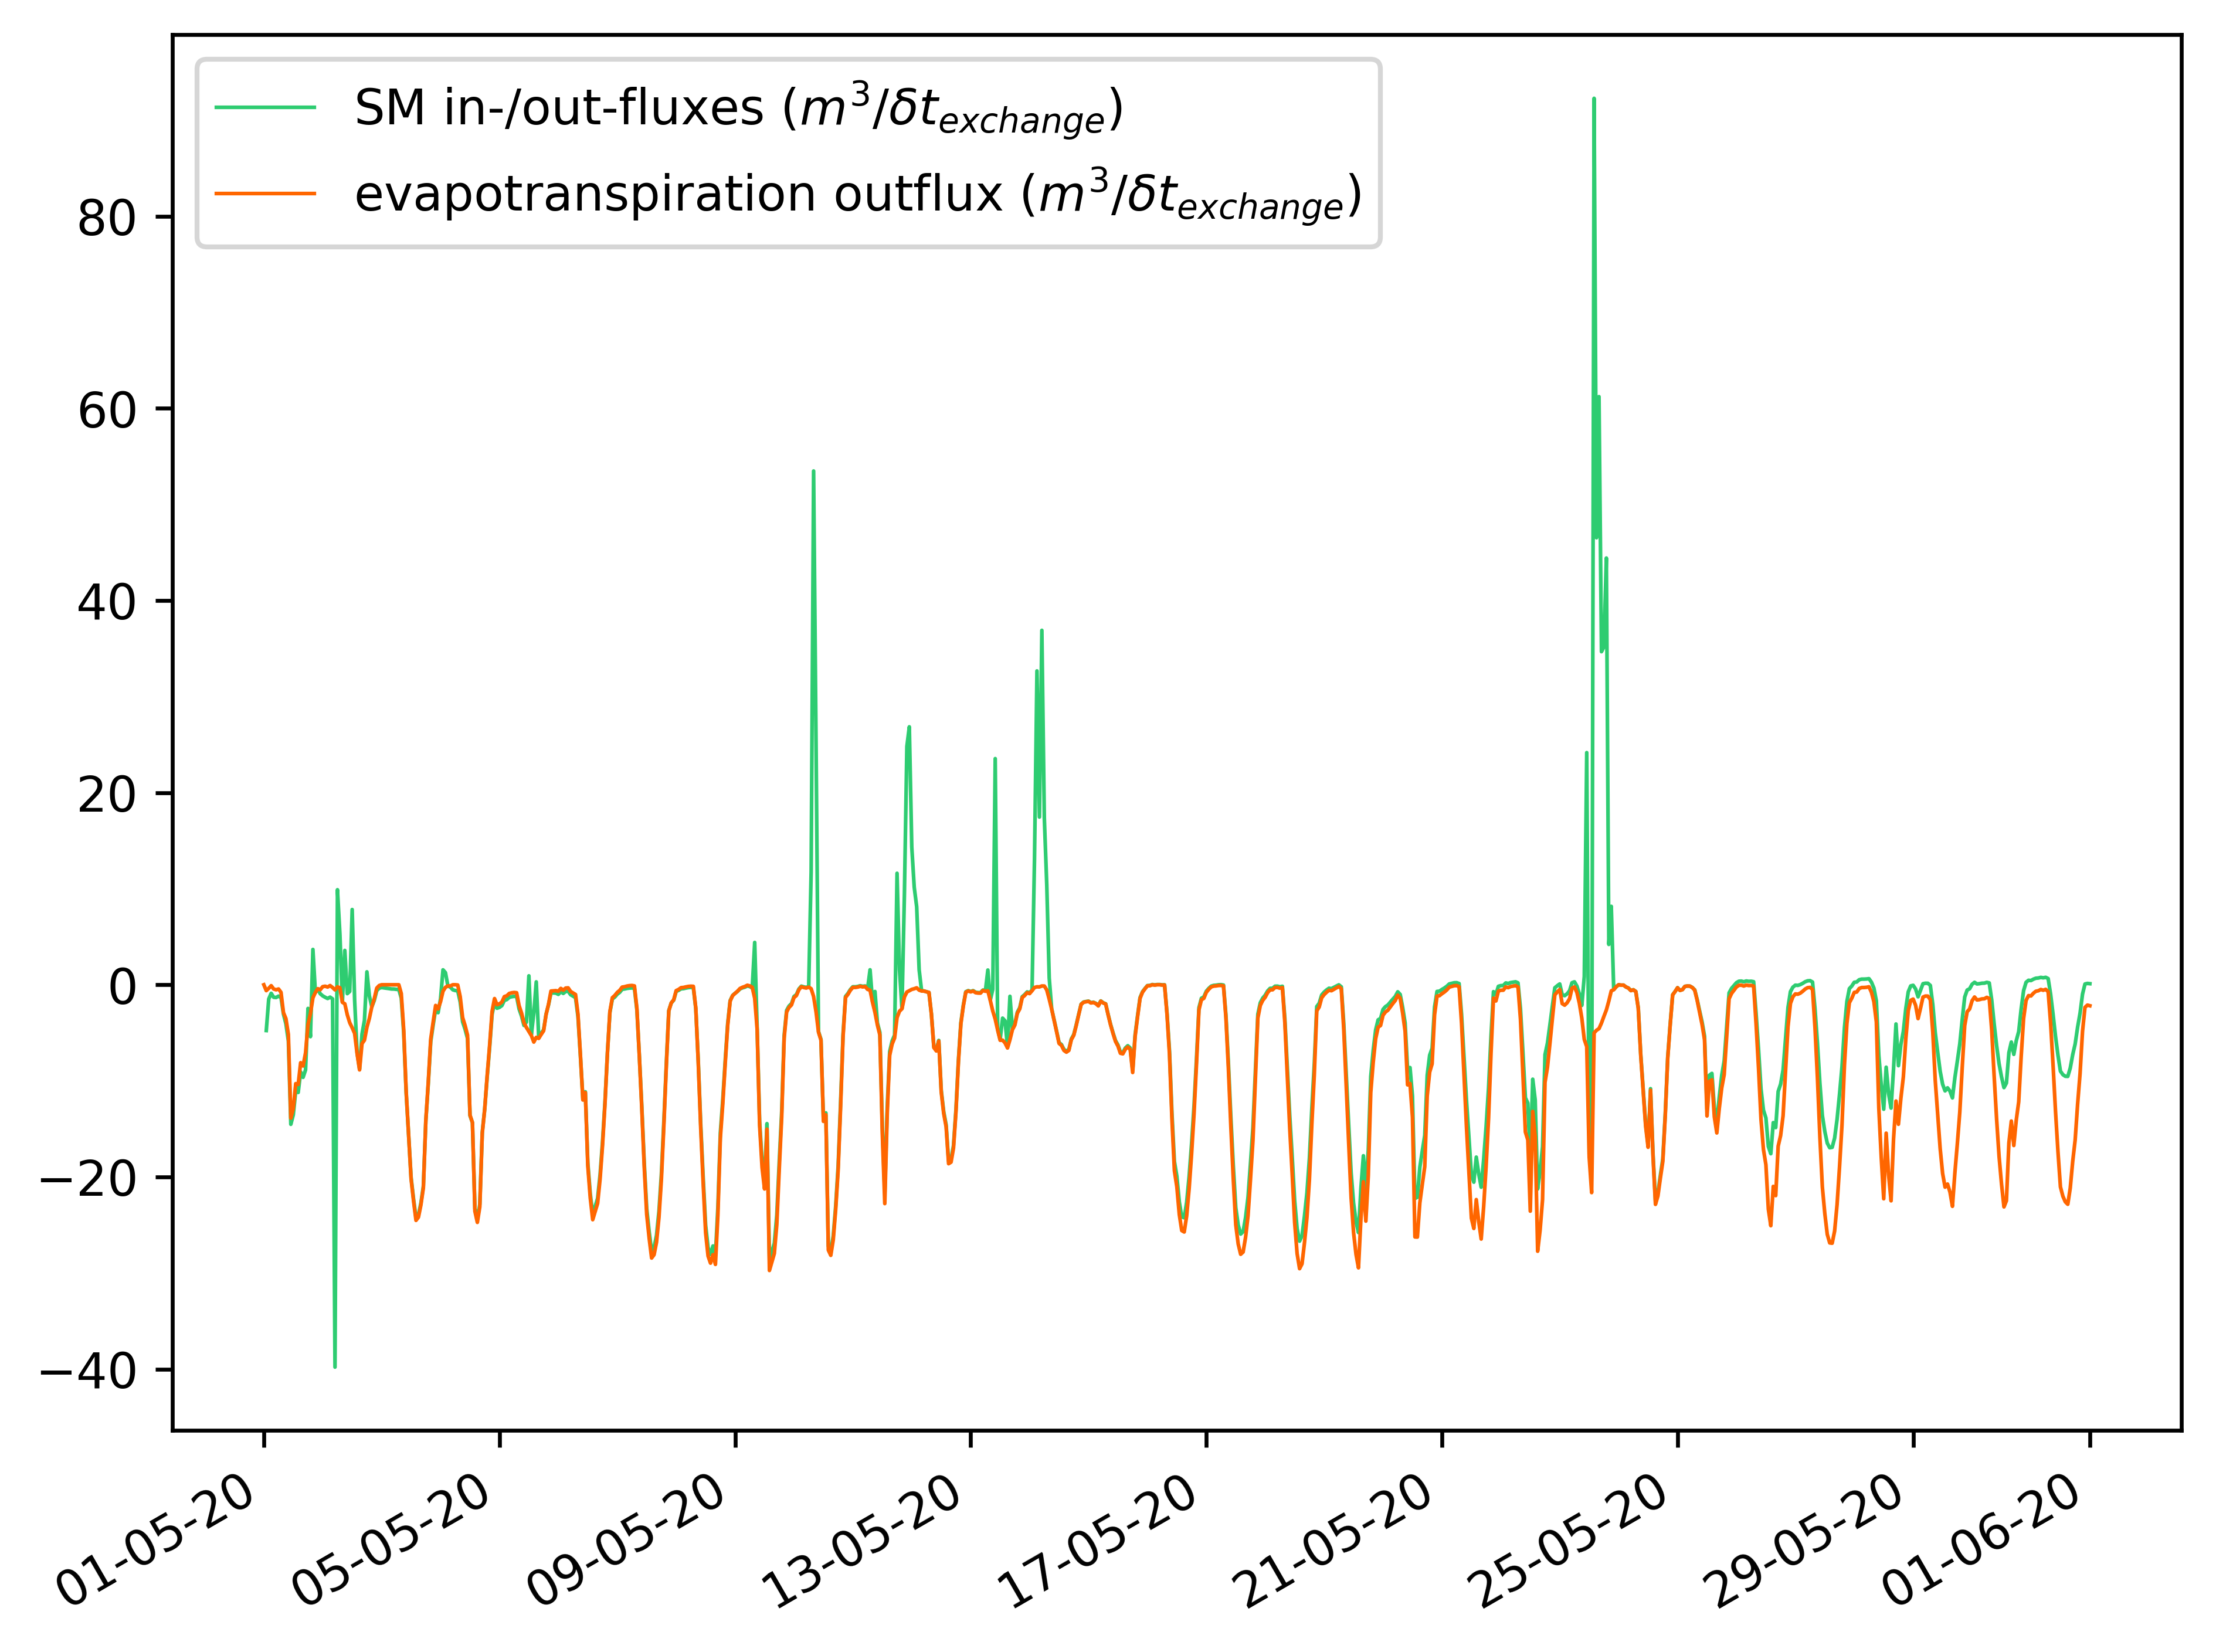
\includegraphics[height=0.42\textheight]{PICTURES/models_res/et_vs_sm}
    \caption{Comparing ET outfluxes with SM storage changes.}
    \label{fig:et_vs_sm}
\end{figure}
\begin{figure}[H]
    \centering
    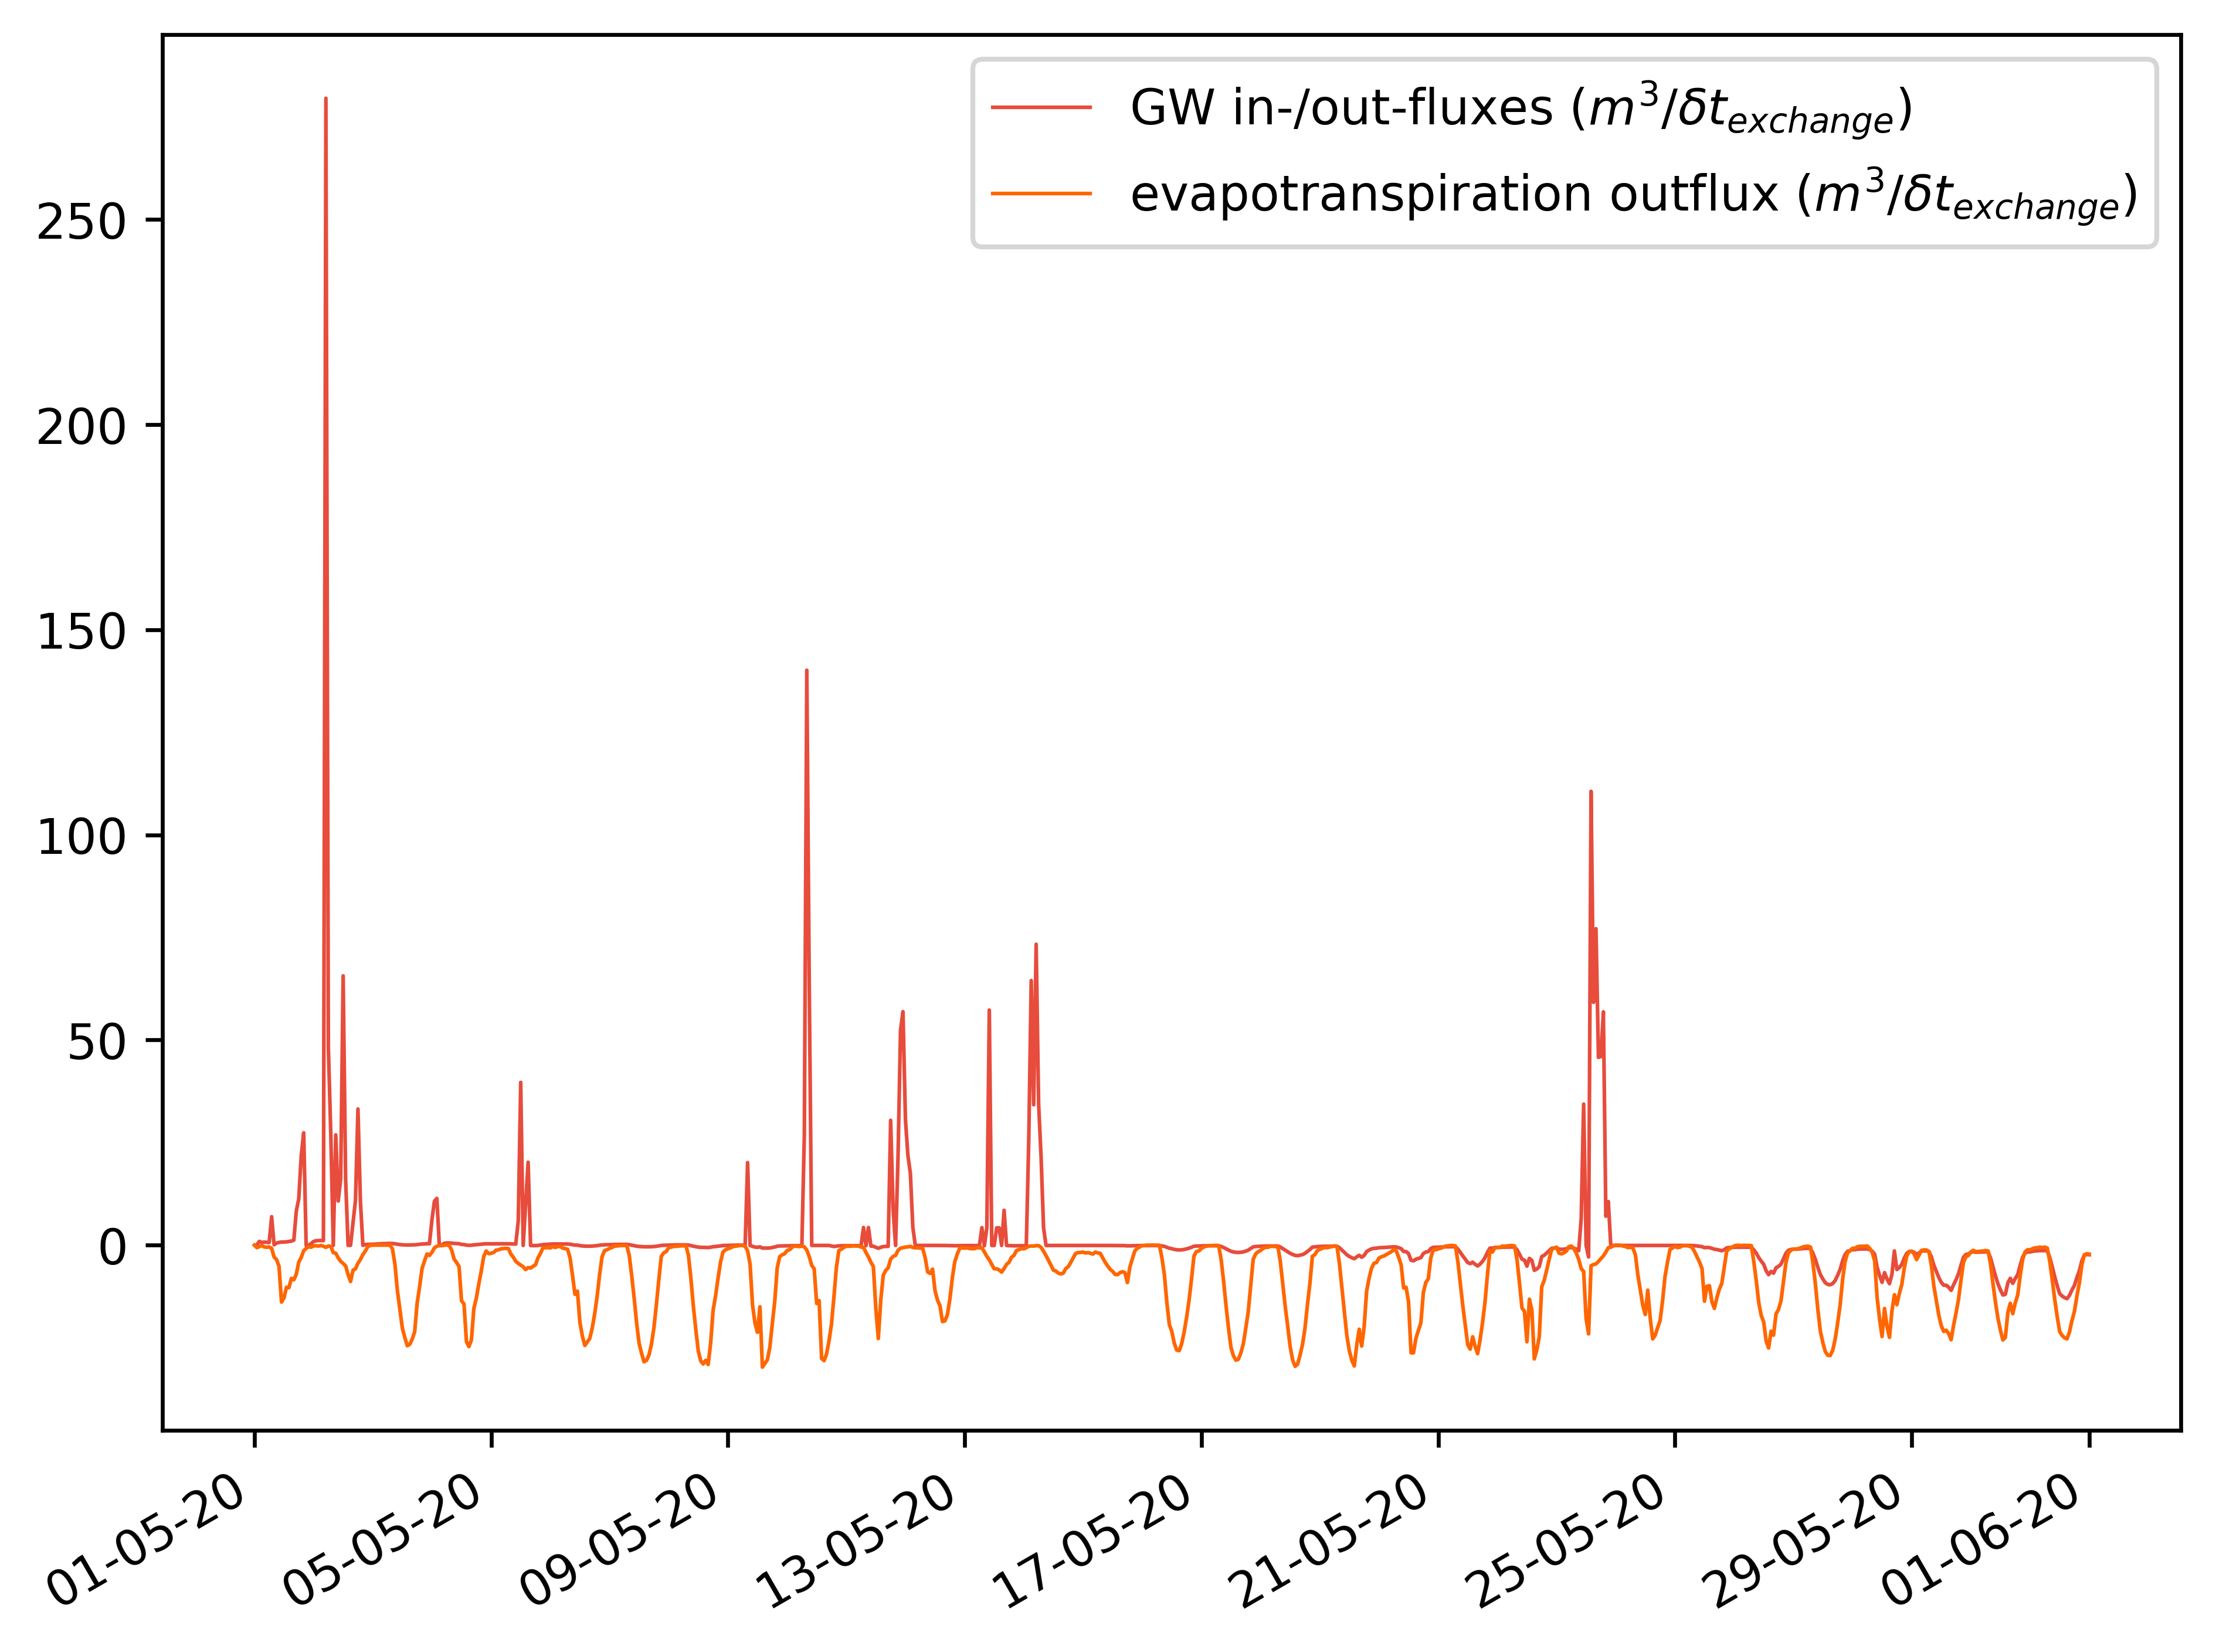
\includegraphics[height=0.42\textheight]{PICTURES/models_res/et_vs_gw}
    \caption{Comparing ET outfluxes with GW storage changes.}
    \label{fig:et_vs_gw}
\end{figure}
\begin{figure}[H]
    \centering
    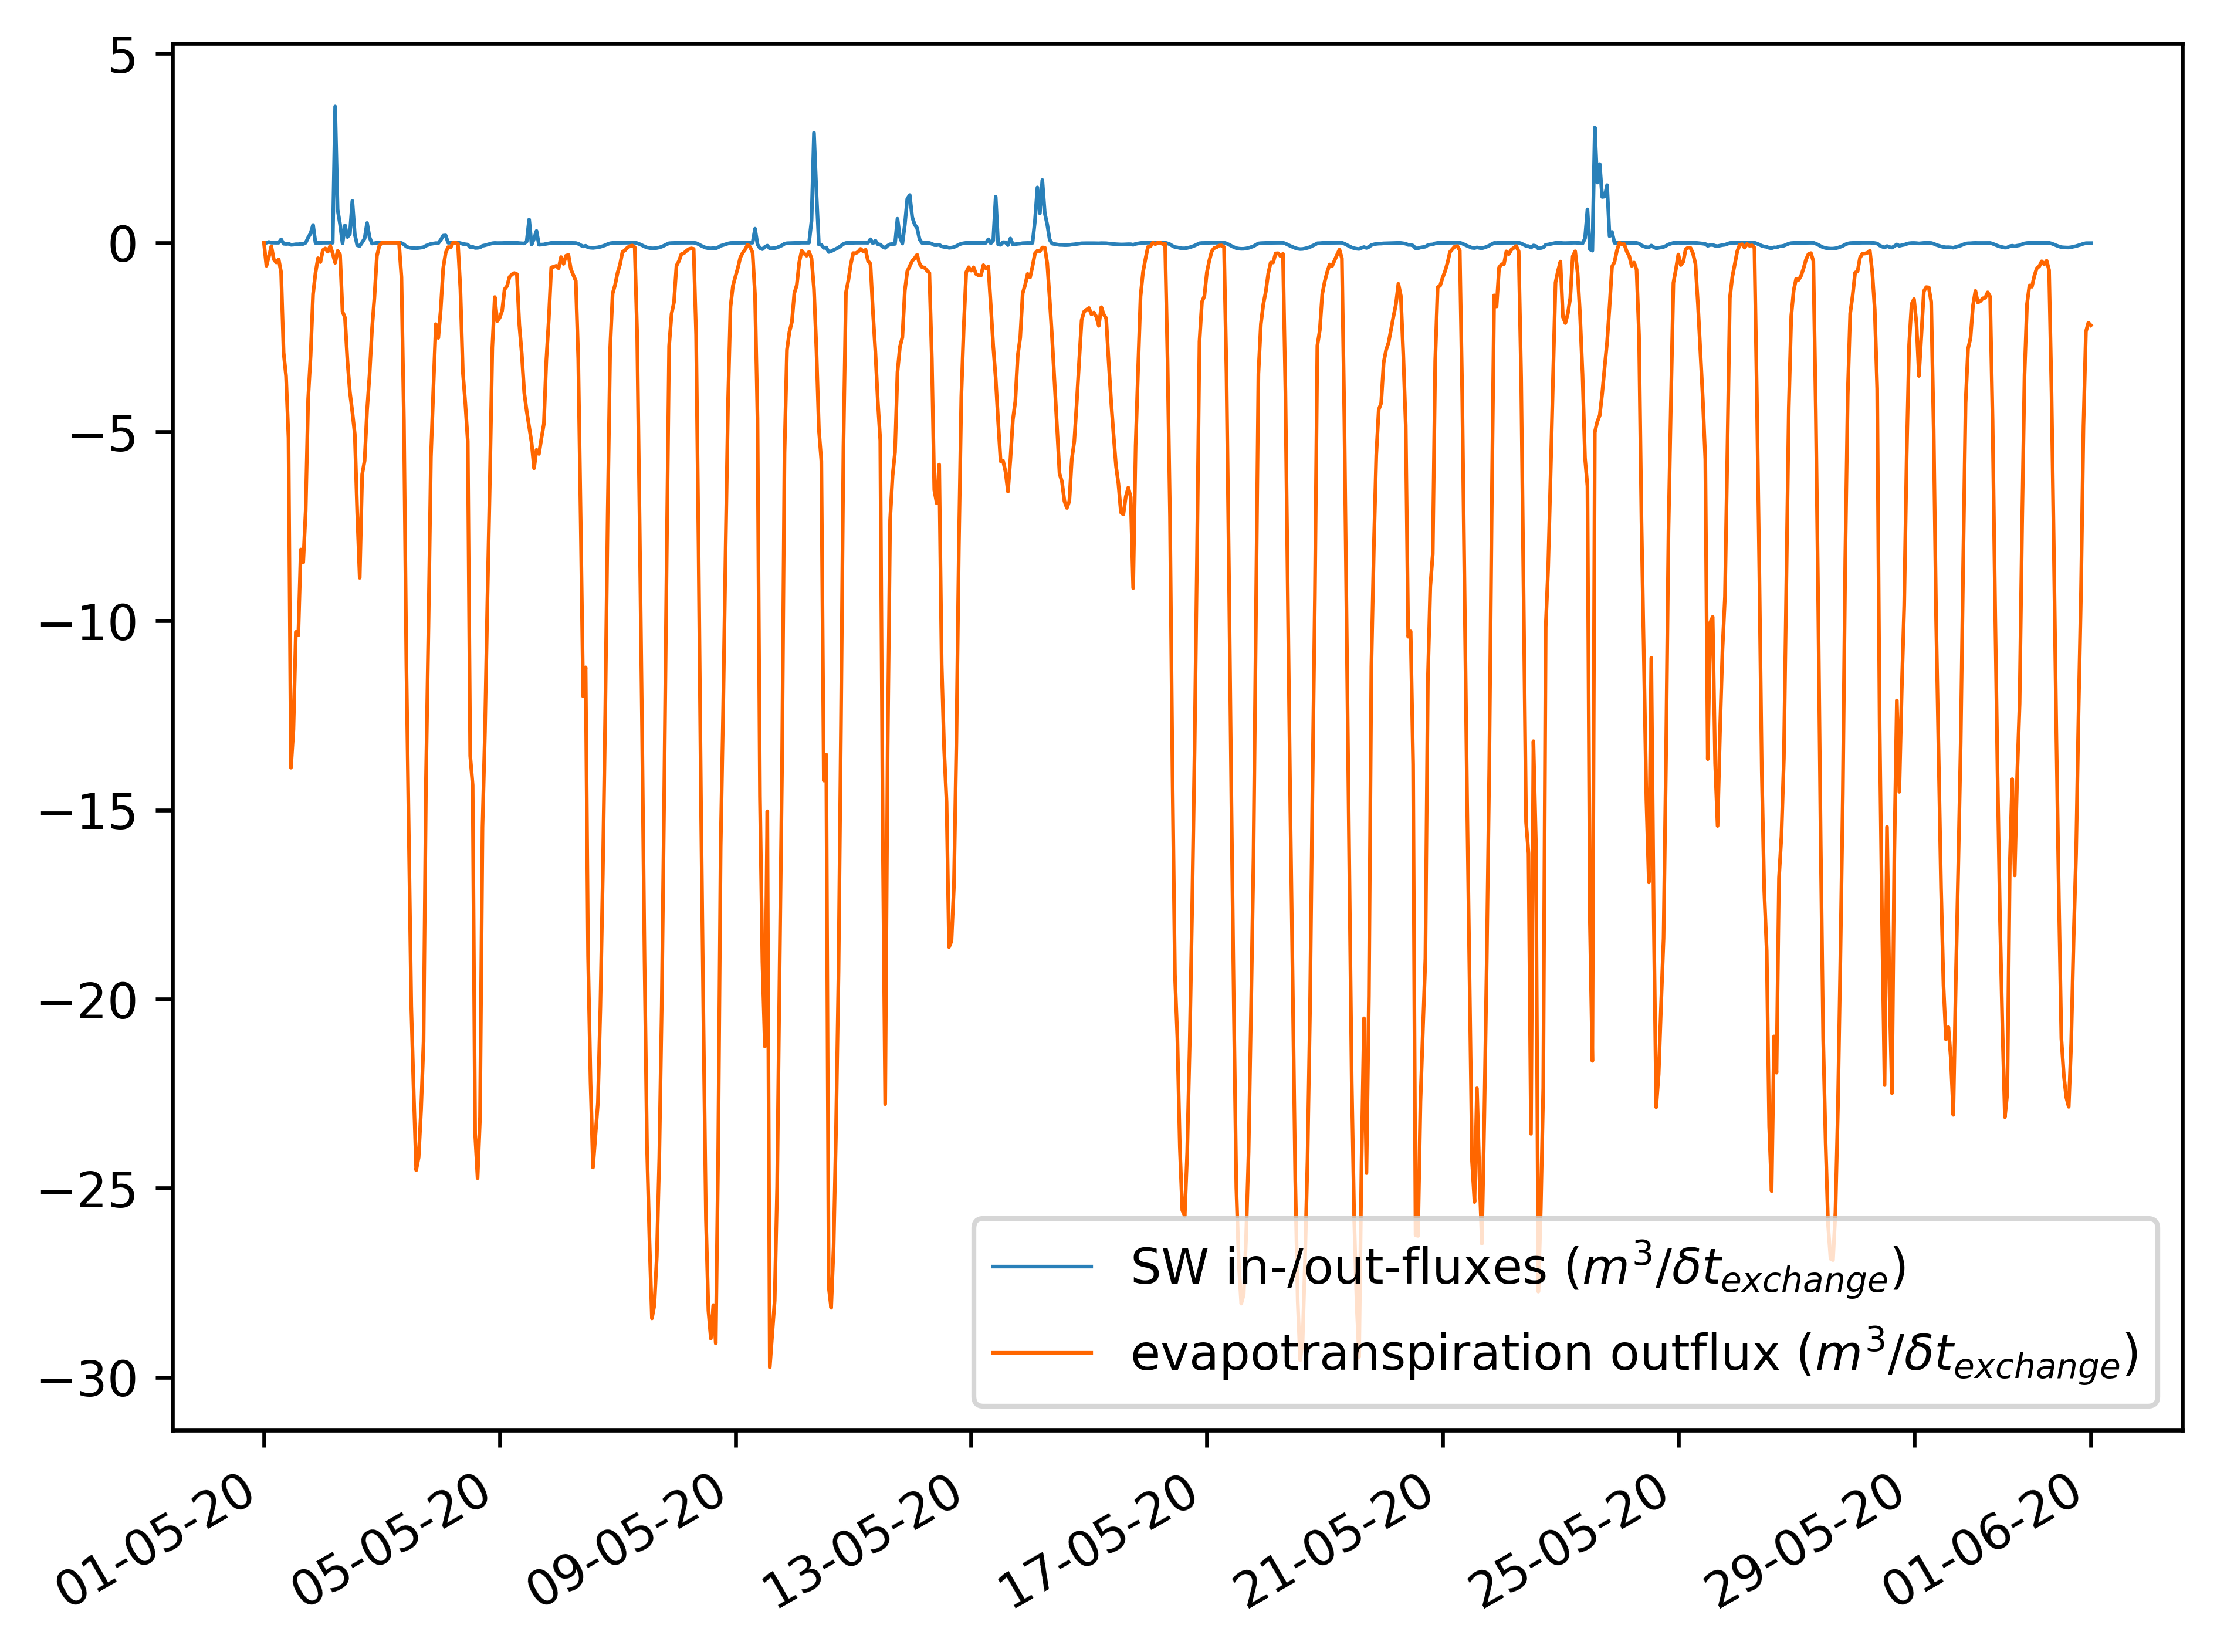
\includegraphics[width=\linewidth]{PICTURES/models_res/et_vs_sw}
    \caption{Comparing ET outfluxes with SW storage changes.}
    \label{fig:et_vs_sw}
\end{figure}


\subsection{Following Precipitation Influx}
The following plots follow the translation of precipitation influx into storage changes.
\\ \\
As seen from Figure \ref{fig:p_vs_gw}, a major portion of the precipitation influx is consistently translated into an influx into the GW storage. The model parameters that control the nature of this translation are $k$ and $\alpha$. Additionally, the SM storage in the previous time-step strongly defines this translation. While $k$ controls the maximum allowable rate of influx into the GW storage, $\alpha$ controls the non-linearity of the influx as discussed in Section \ref{GWSWEX_vs_Richards}.
\\ \\
A good portion of the precipitation influx is translated into an influx into the SM storage term as well. The nature of this translation is defined by the model parameters $\beta$, $n$, and $m$. Furthermore, it is also strongly defined by the SM storage in the previous time-step. While $\beta$ controls the non-linearity, $n$ defines the maximum allowable SM storage, and $m$ defines $SM_\textrm{min}$, beyond which the SM storage is not reducible, as discussed in Section \ref{GWSWEX_vs_Richards}.
\\ \\
As was expected for this simulation period, not much of the precipitation influx was translated into influxes to the SW storage term. The nature of this translation is controlled by the nature of translations of precipitation influxes into the GW and SM terms, as discussed in \ref{fig:GWSWEX_flow}.

\begin{figure}[H]
\centering
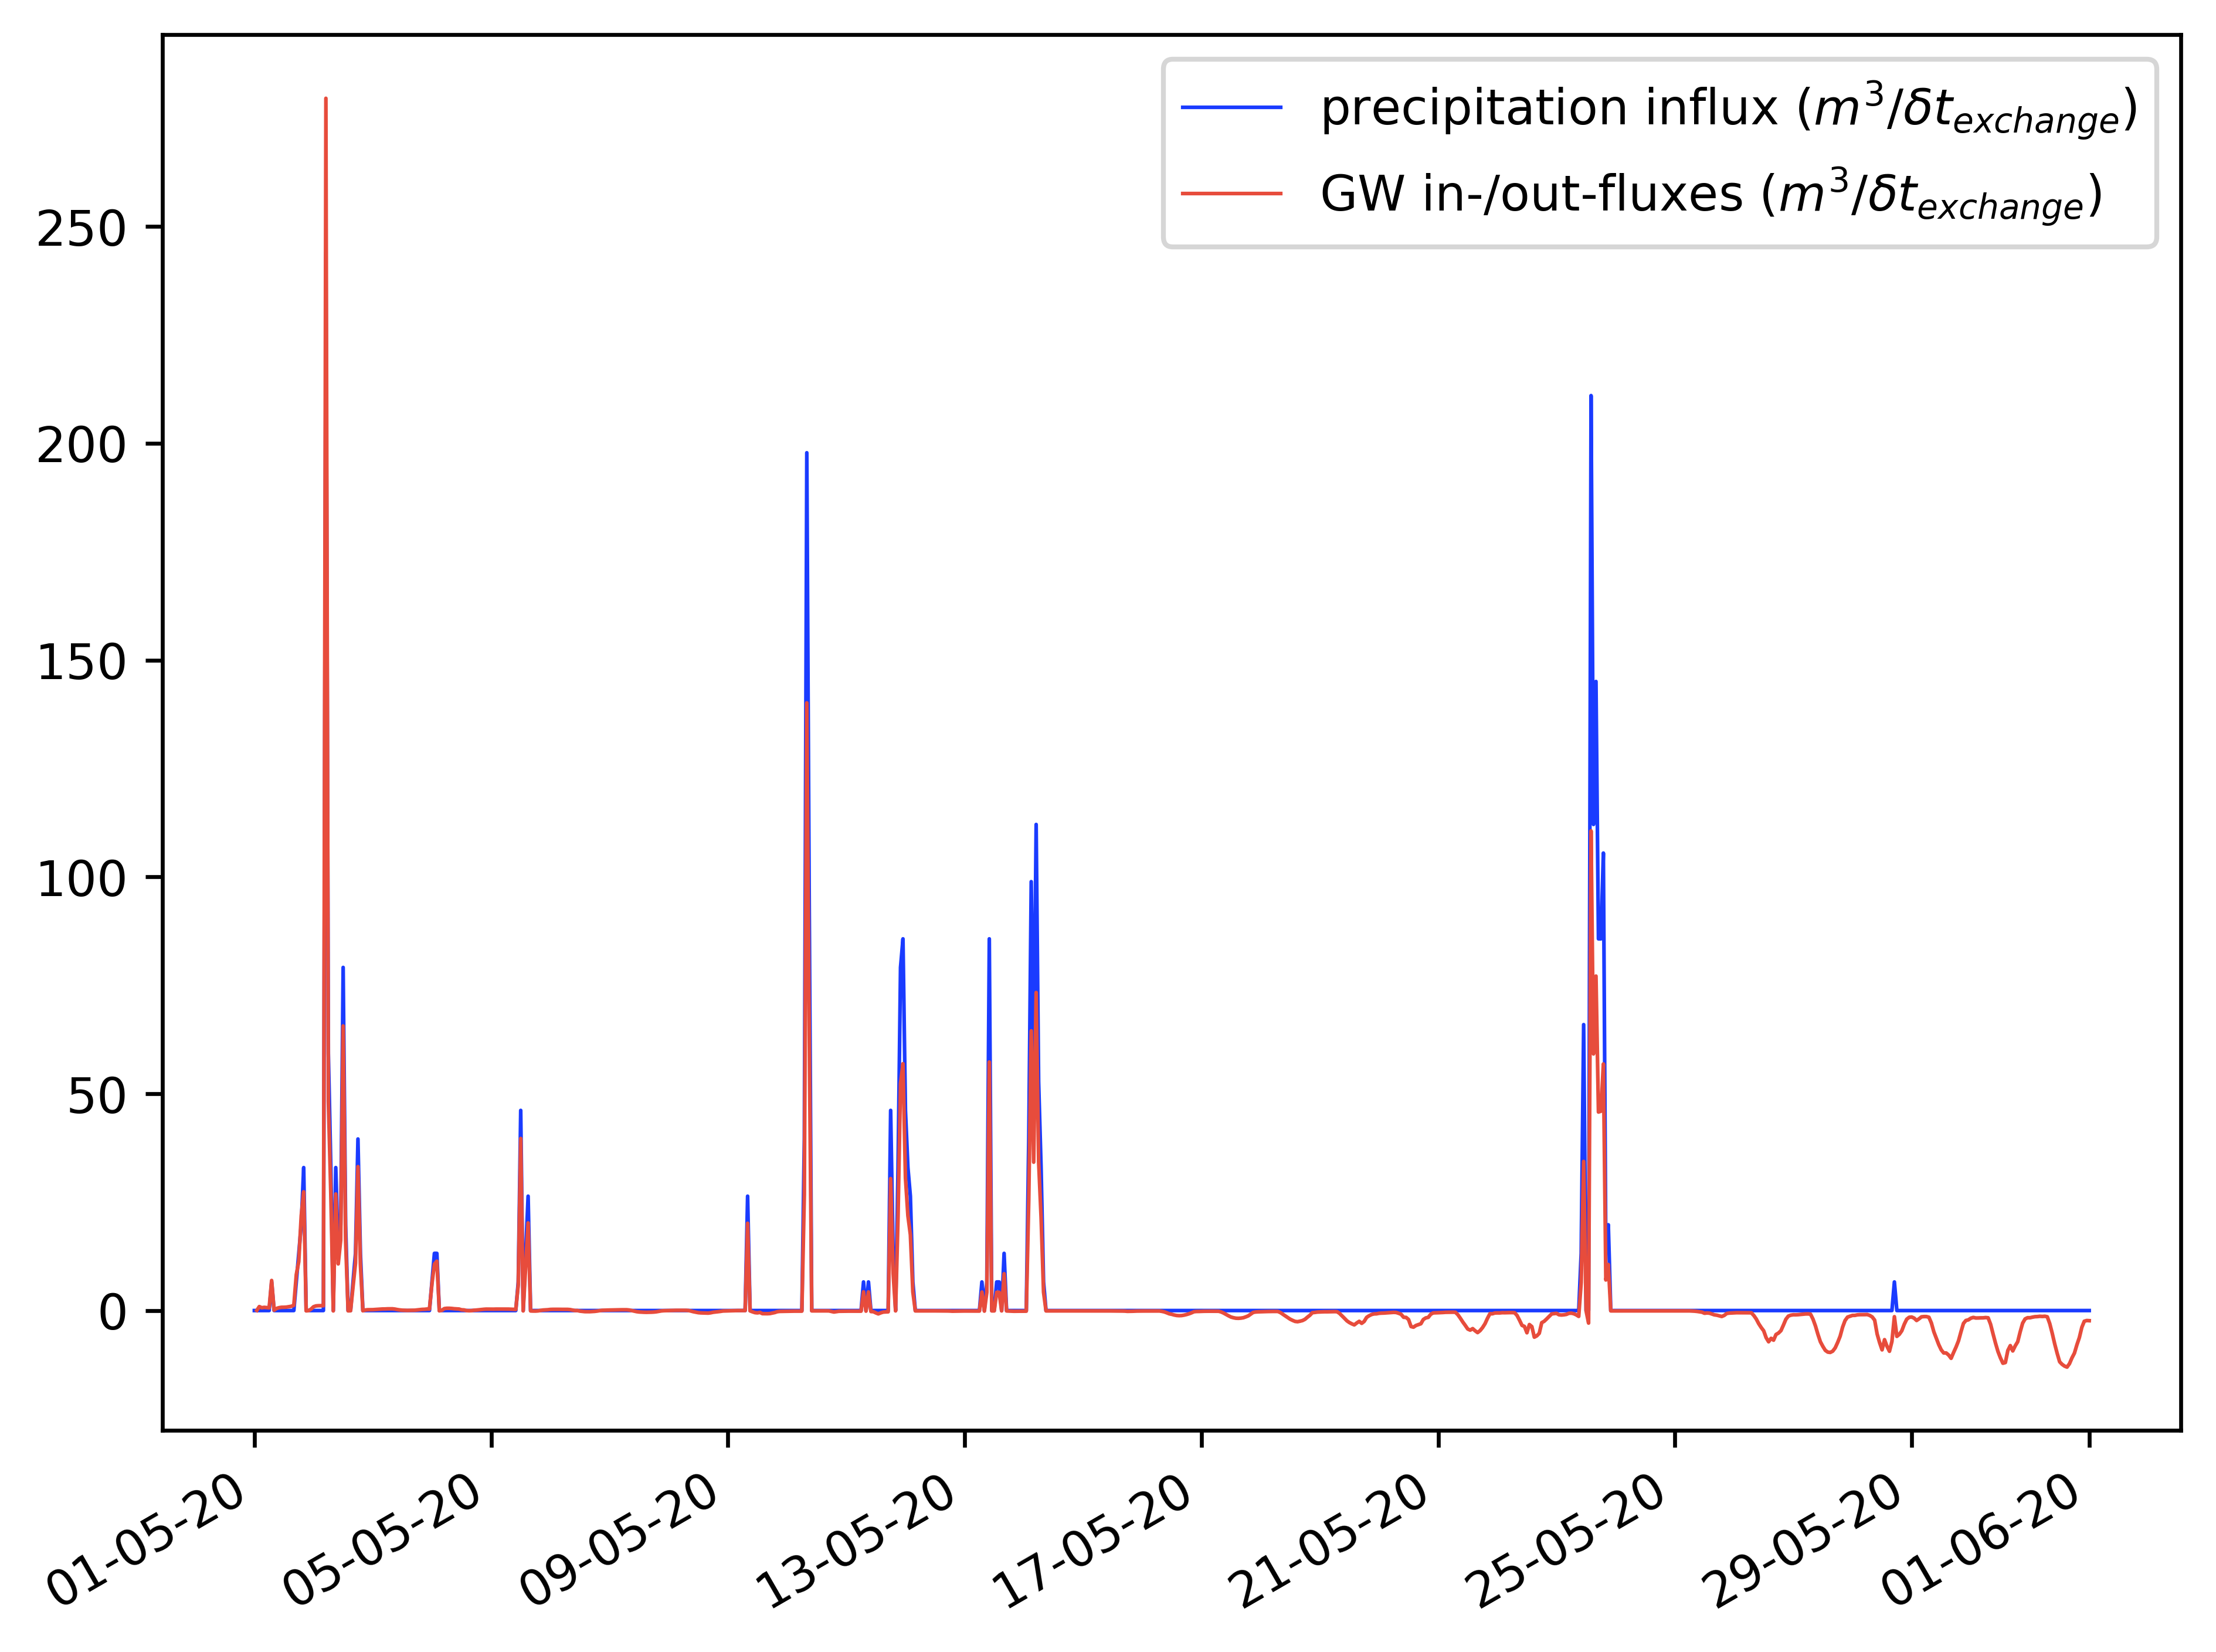
\includegraphics[width=\linewidth]{PICTURES/models_res/p_vs_gw}
\caption{Comparing P influxes with GW storage changes.}\label{fig:p_vs_gw}
\end{figure}
\begin{figure}[H]
\centering
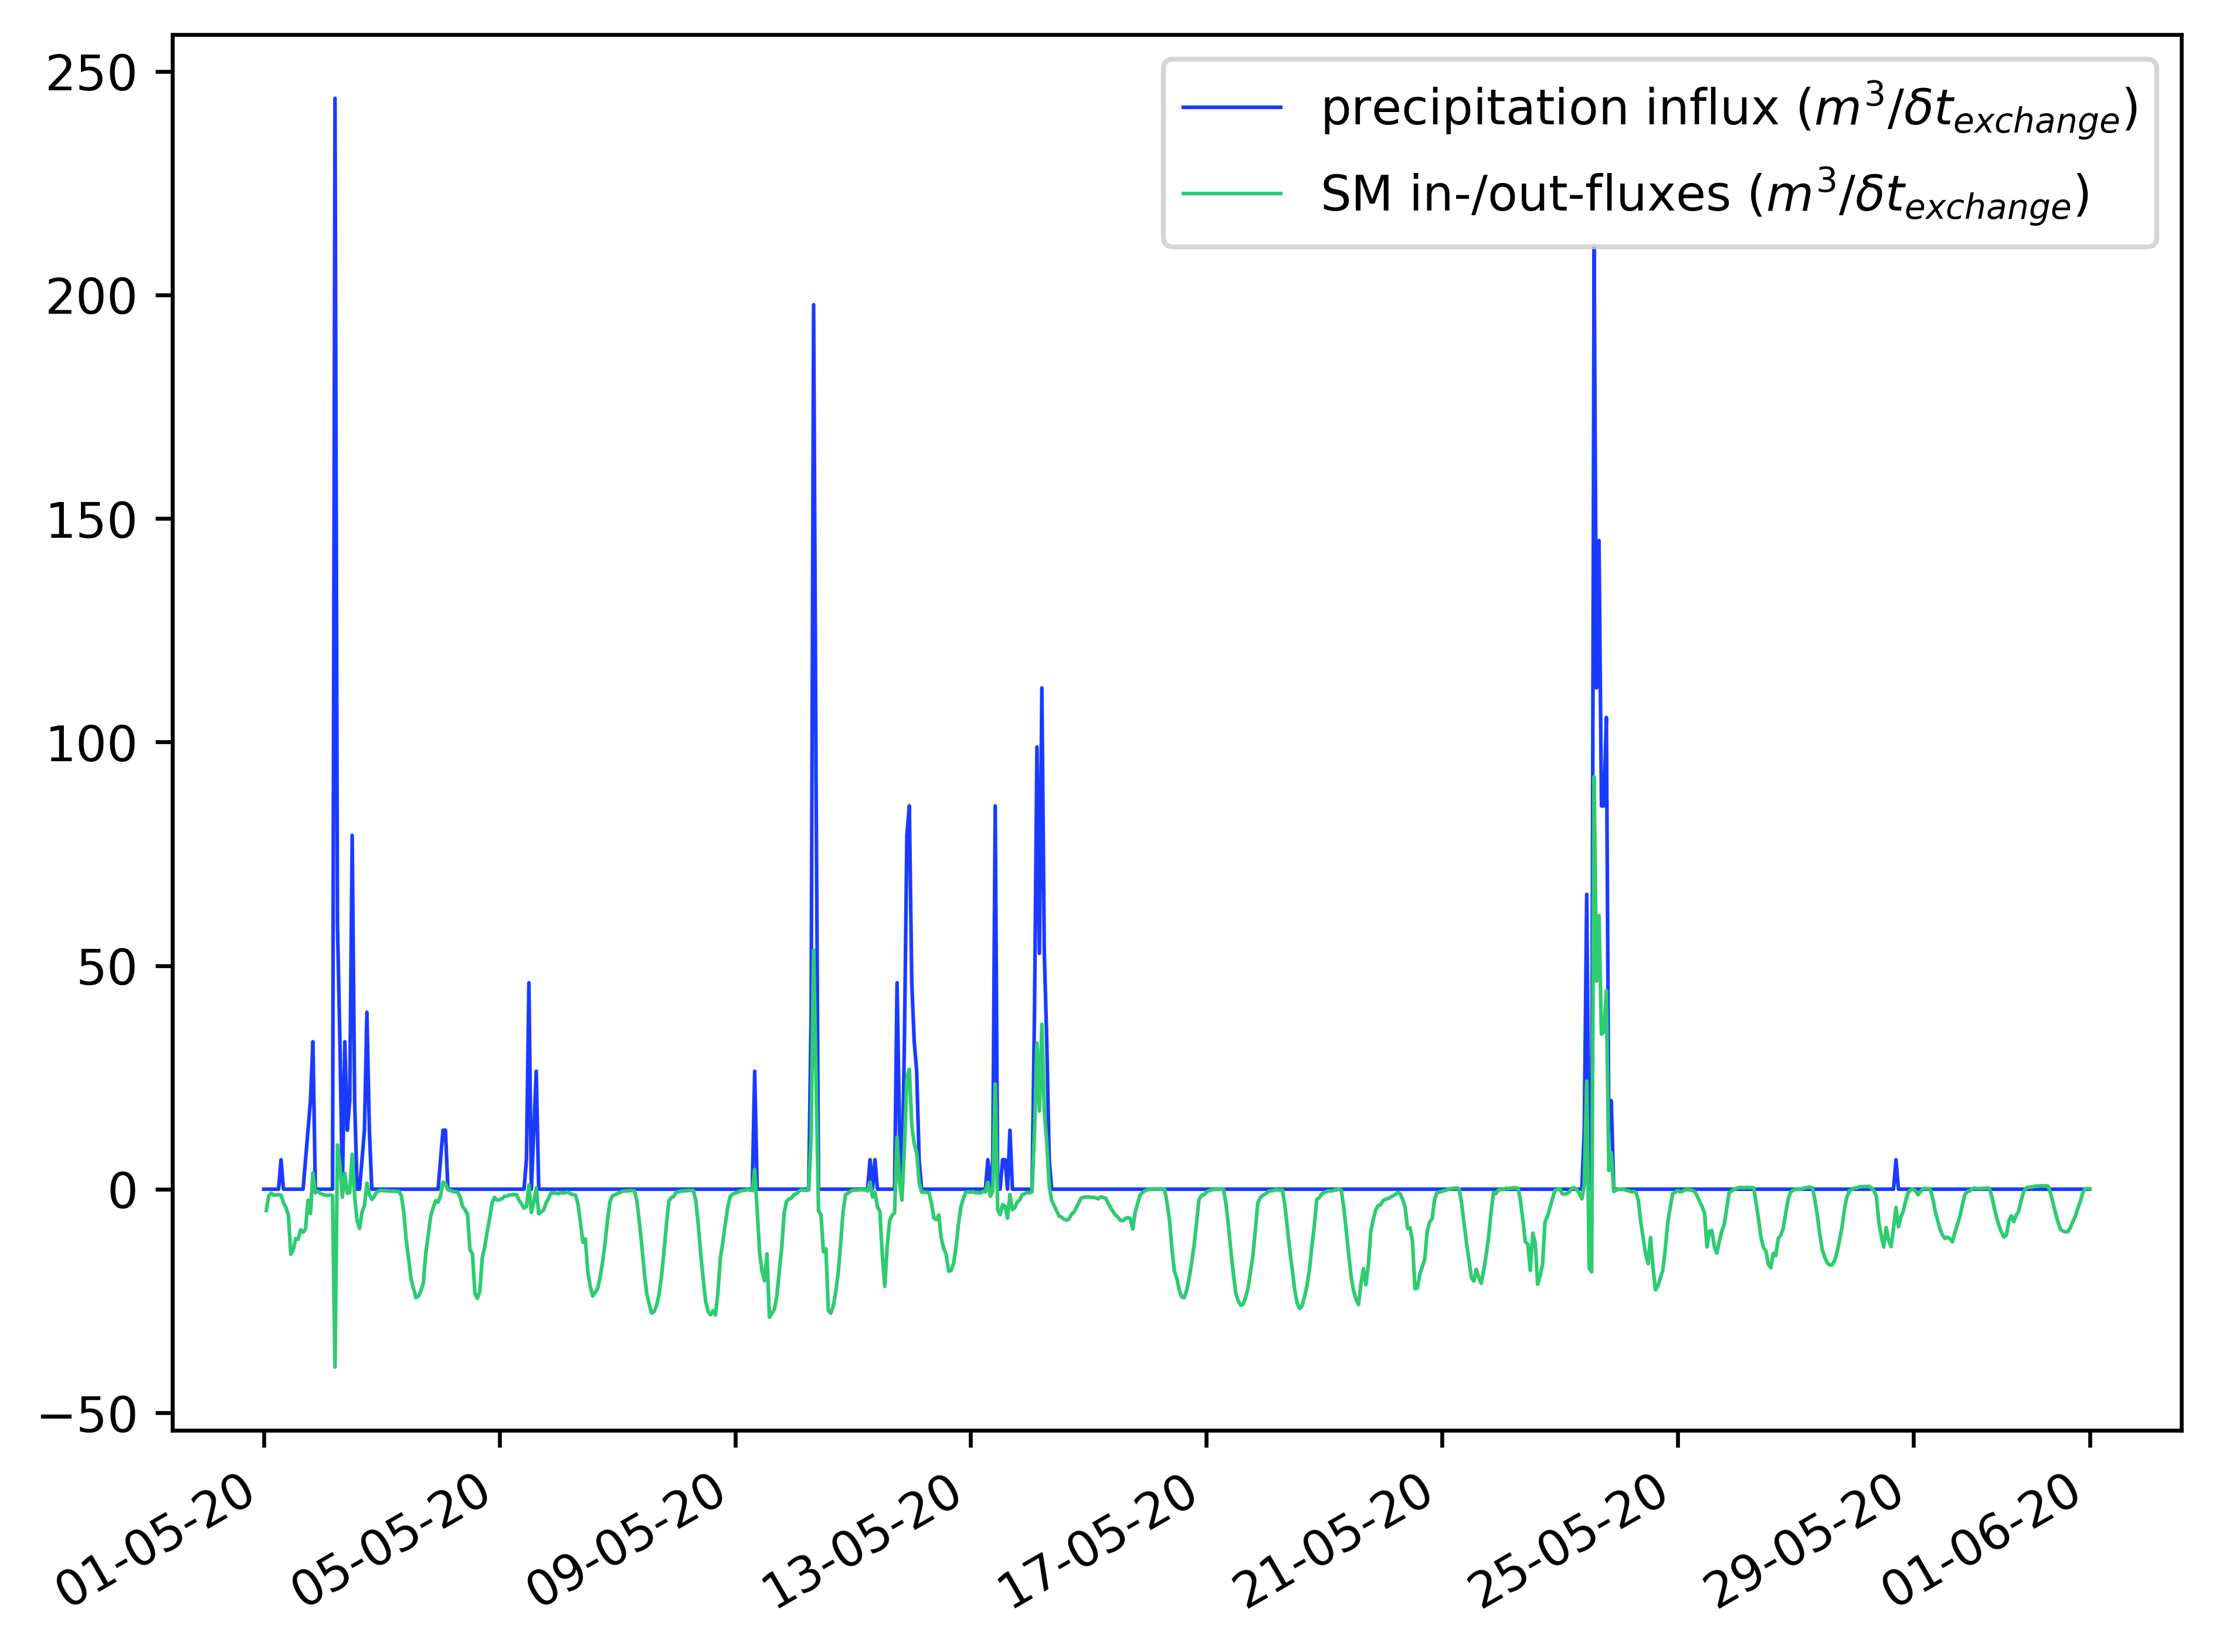
\includegraphics[height=0.42\textheight]{PICTURES/models_res/p_vs_sm}
\caption{Comparing P influxes with SM storage changes.}\label{fig:p_vs_sm}
\end{figure}
\begin{figure}[H]
\centering
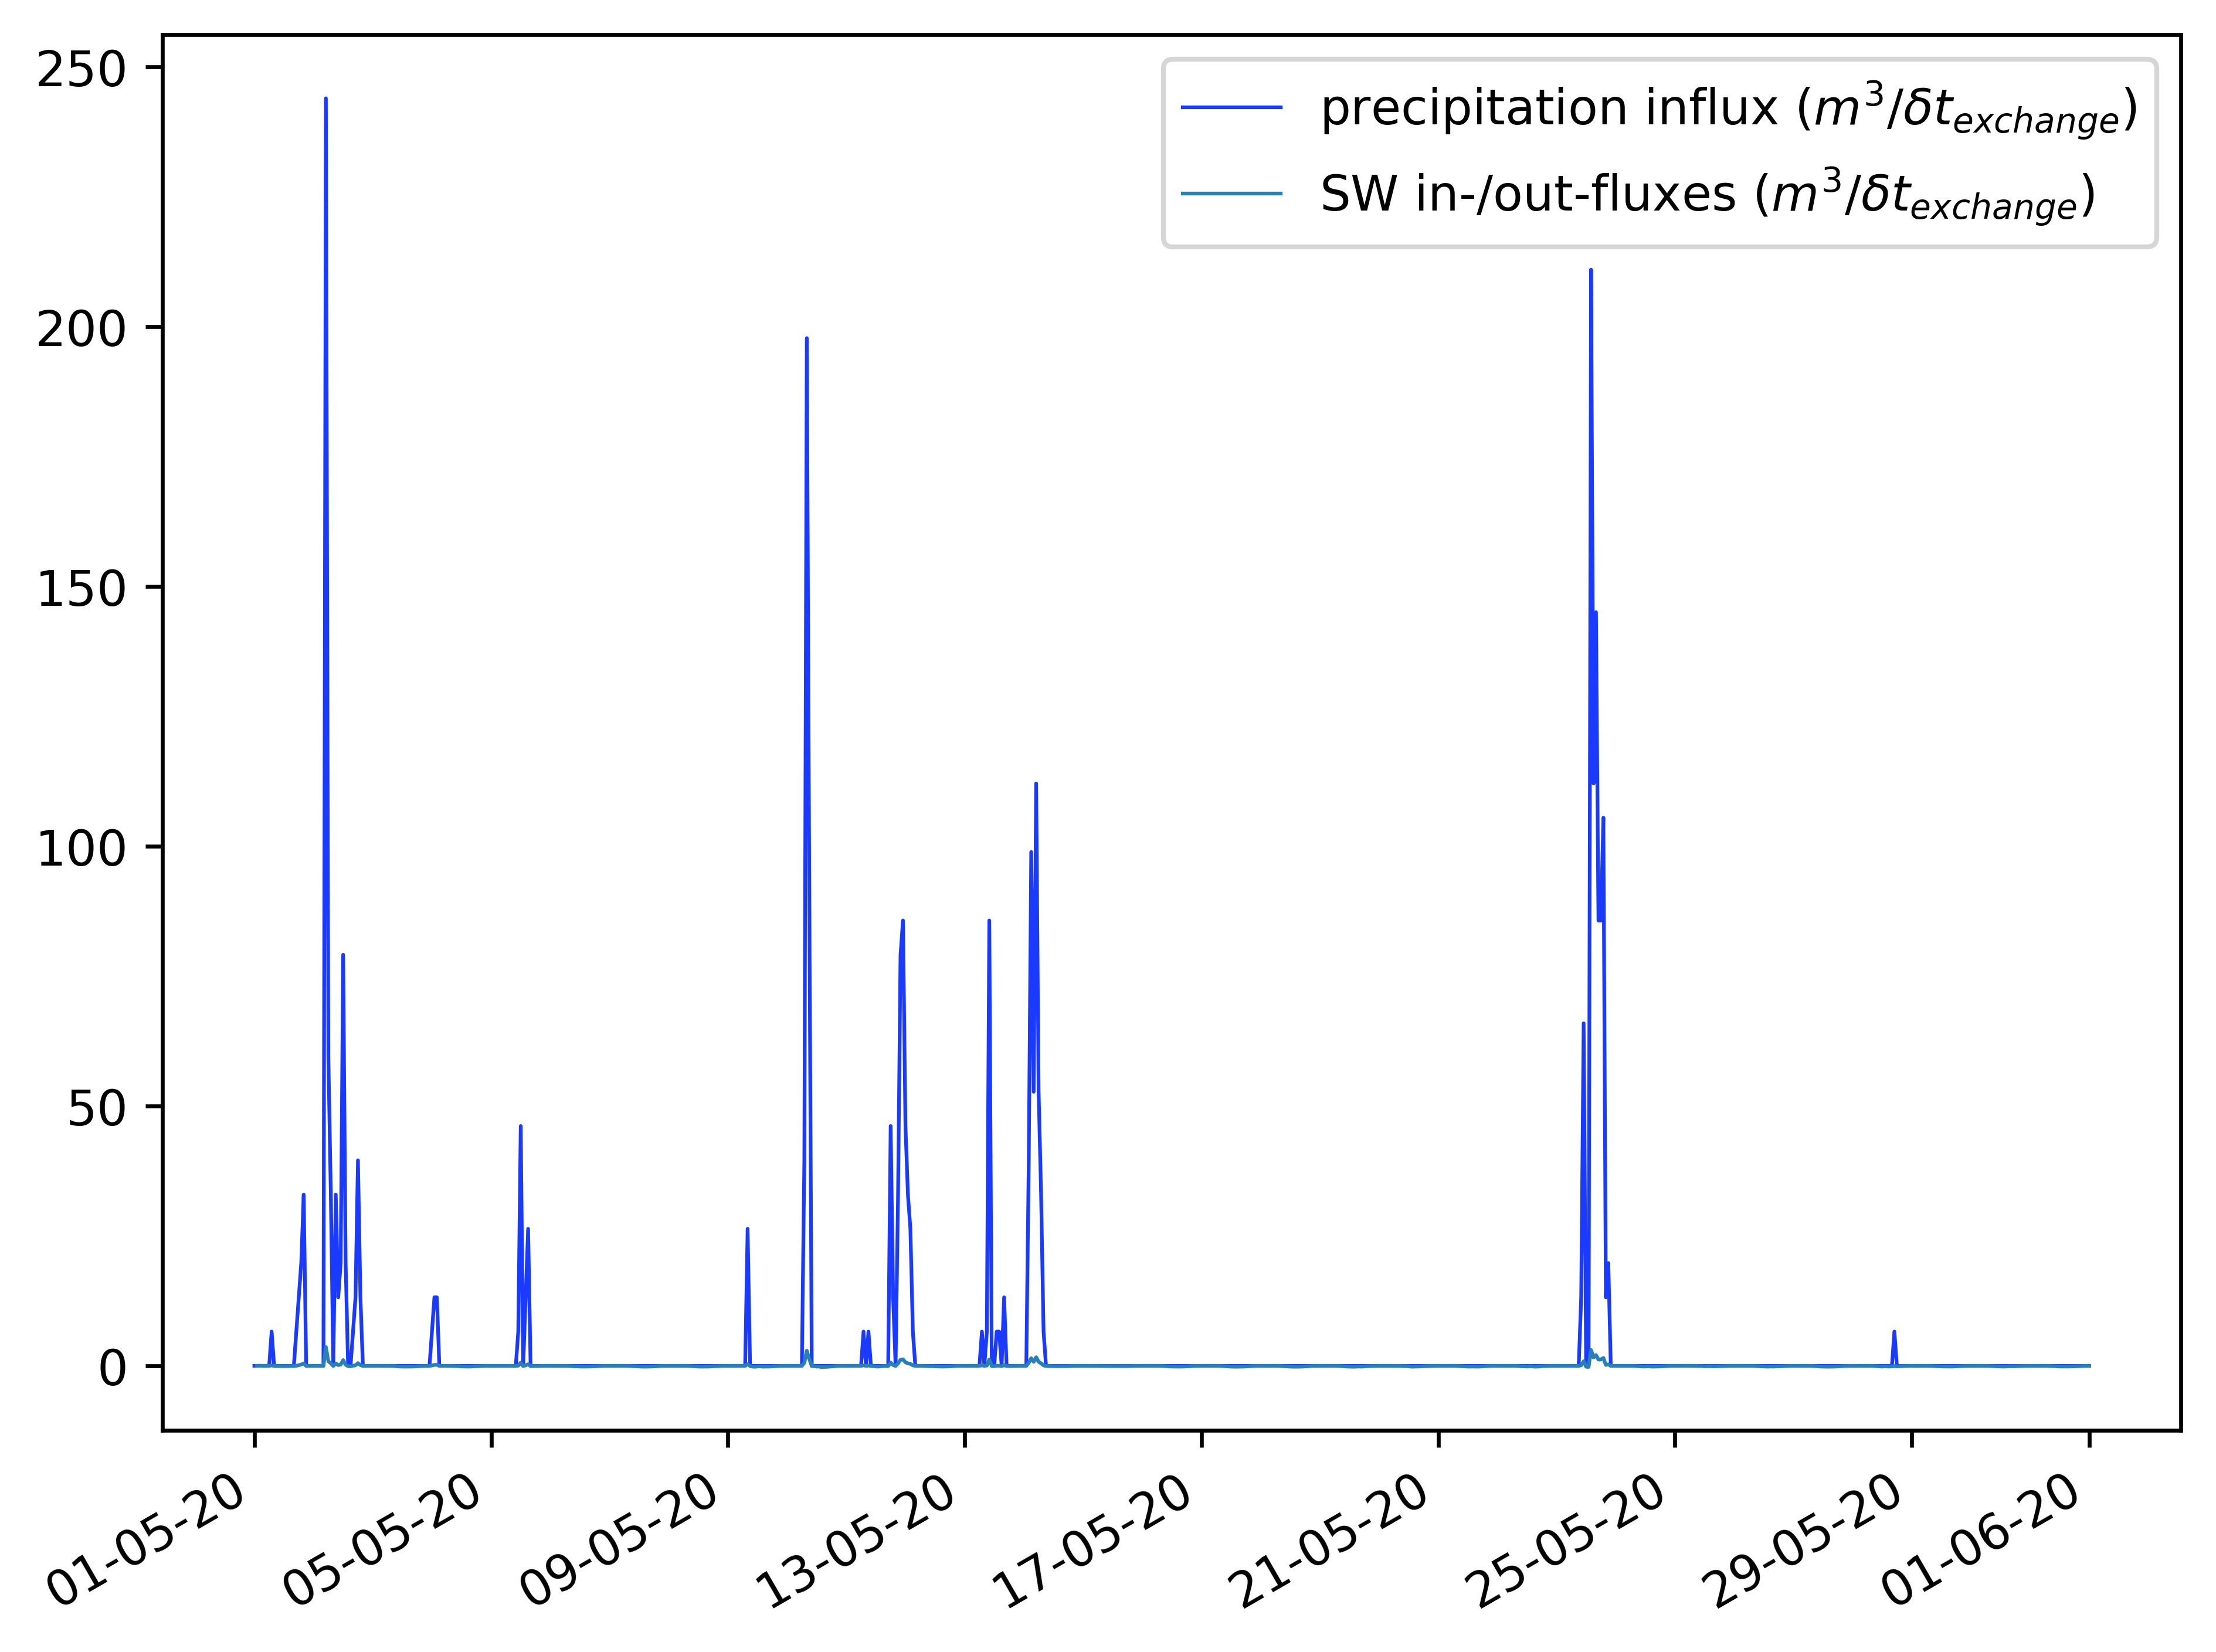
\includegraphics[height=0.42\textheight]{PICTURES/models_res/p_vs_sw}
\caption{Comparing P influxes with SW storage changes.}\label{fig:p_vs_sw}
\end{figure}

\subsection{Following GW and SM Fluxes}
As discussed in \ref{fig:GWSWEX_flow}, an increase in GW levels imply a reduction in the unsaturated zone and thus the effective pore volume in the unsaturated zone. From this, it is to be expected that a considerable influx into the GW storage must imply a considerable outflux from the SM storage. This may be observed in Figure \ref{fig:sm_vs_gw}.
\begin{figure}[H] 
\centering
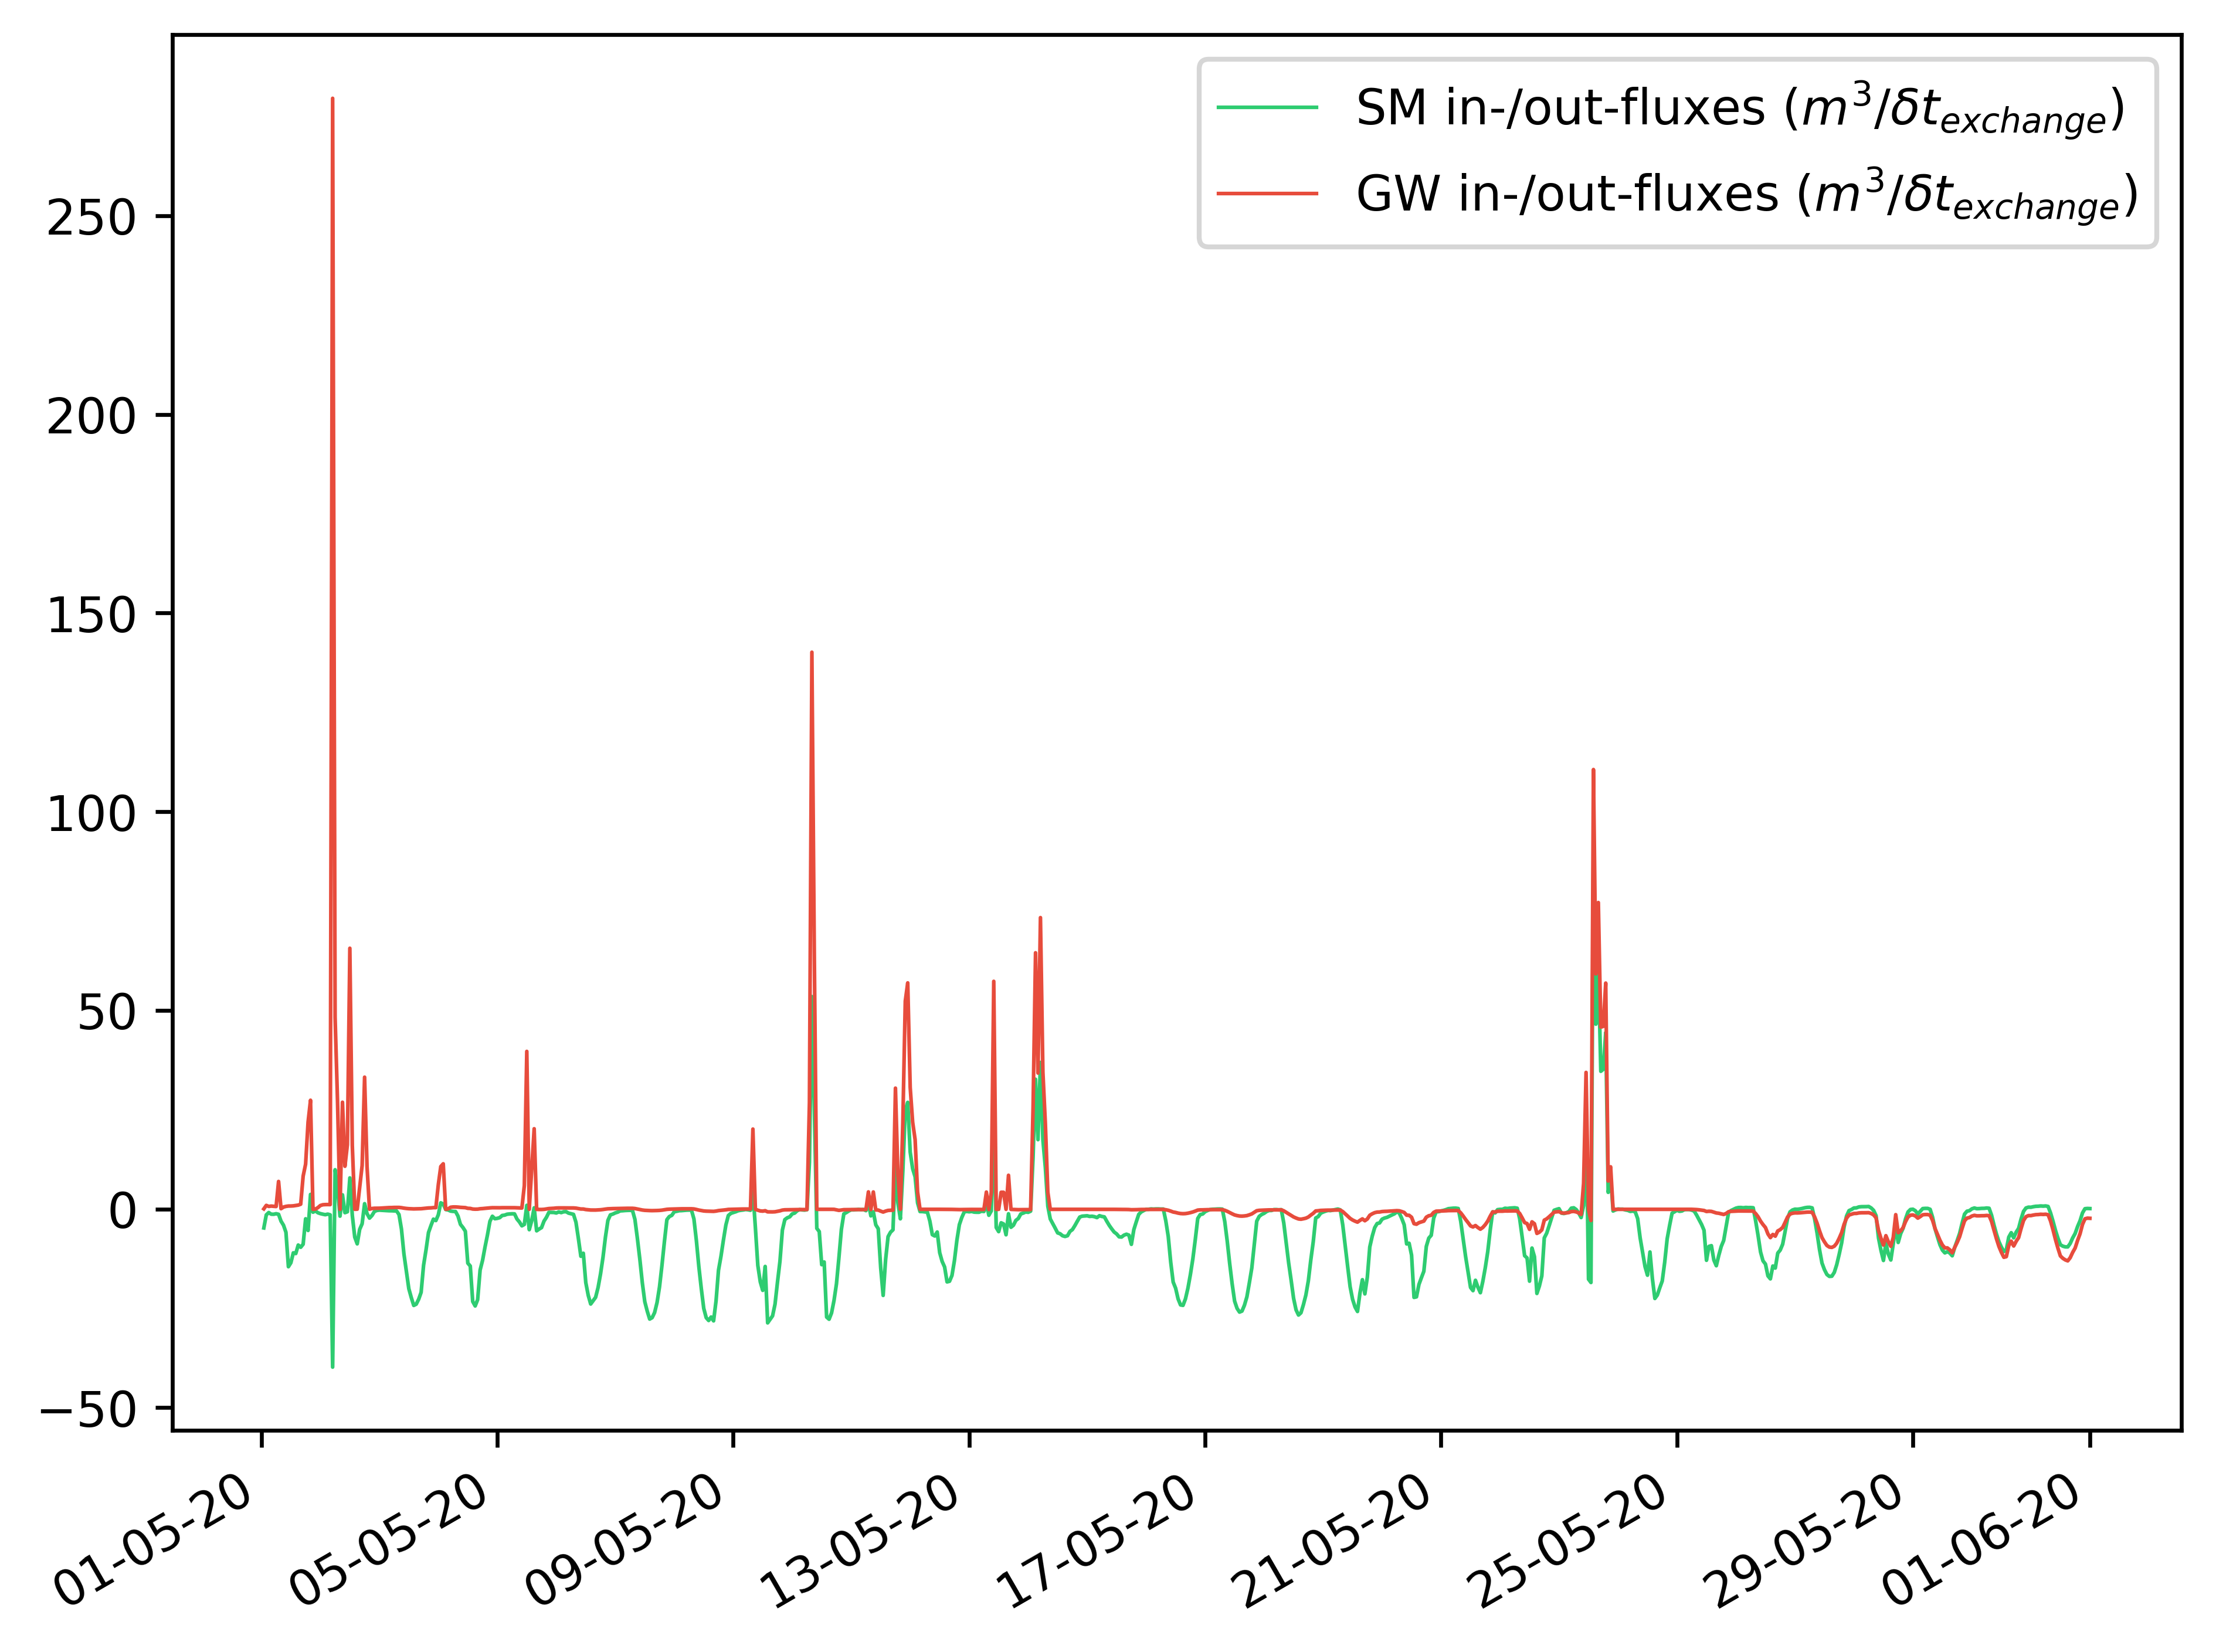
\includegraphics[height=0.42\textheight]{PICTURES/models_res/sm_vs_gw}
\caption{Comparing SM and GW storage changes.}\label{fig:sm_vs_gw}
\end{figure}
Further, to maintain $SM_\textrm{min}$, there outflux from GW is translated into influx into SM, as seen in Figures \ref{fig:sm_vs_gw}, \ref{fig:p_vs_gw}, and \ref{fig:p_vs_sm} starting roughly from 26-05-2020 to the end of the simulation period.

\section{Storages}
Figure \ref{fig:mf6_res} shows the hydraulic heads in the GW model at the end of the simulation. Comparing it with \ref{fig:mf6_ic_strt}, one may notice that the hydraulic heads in the unconfined aquifer has significantly decreased, owing to the dominance of ET outfluxes.
\\ \\
The dominant ET outfluxes have resulted in a reduction in the SM storage as well, as observed in \ref{fig:sm_res}. One may observe that the reduction in SM is stronger along the dewatering stream.

\begin{figure}[H]
\minipage{0.32\textwidth}
  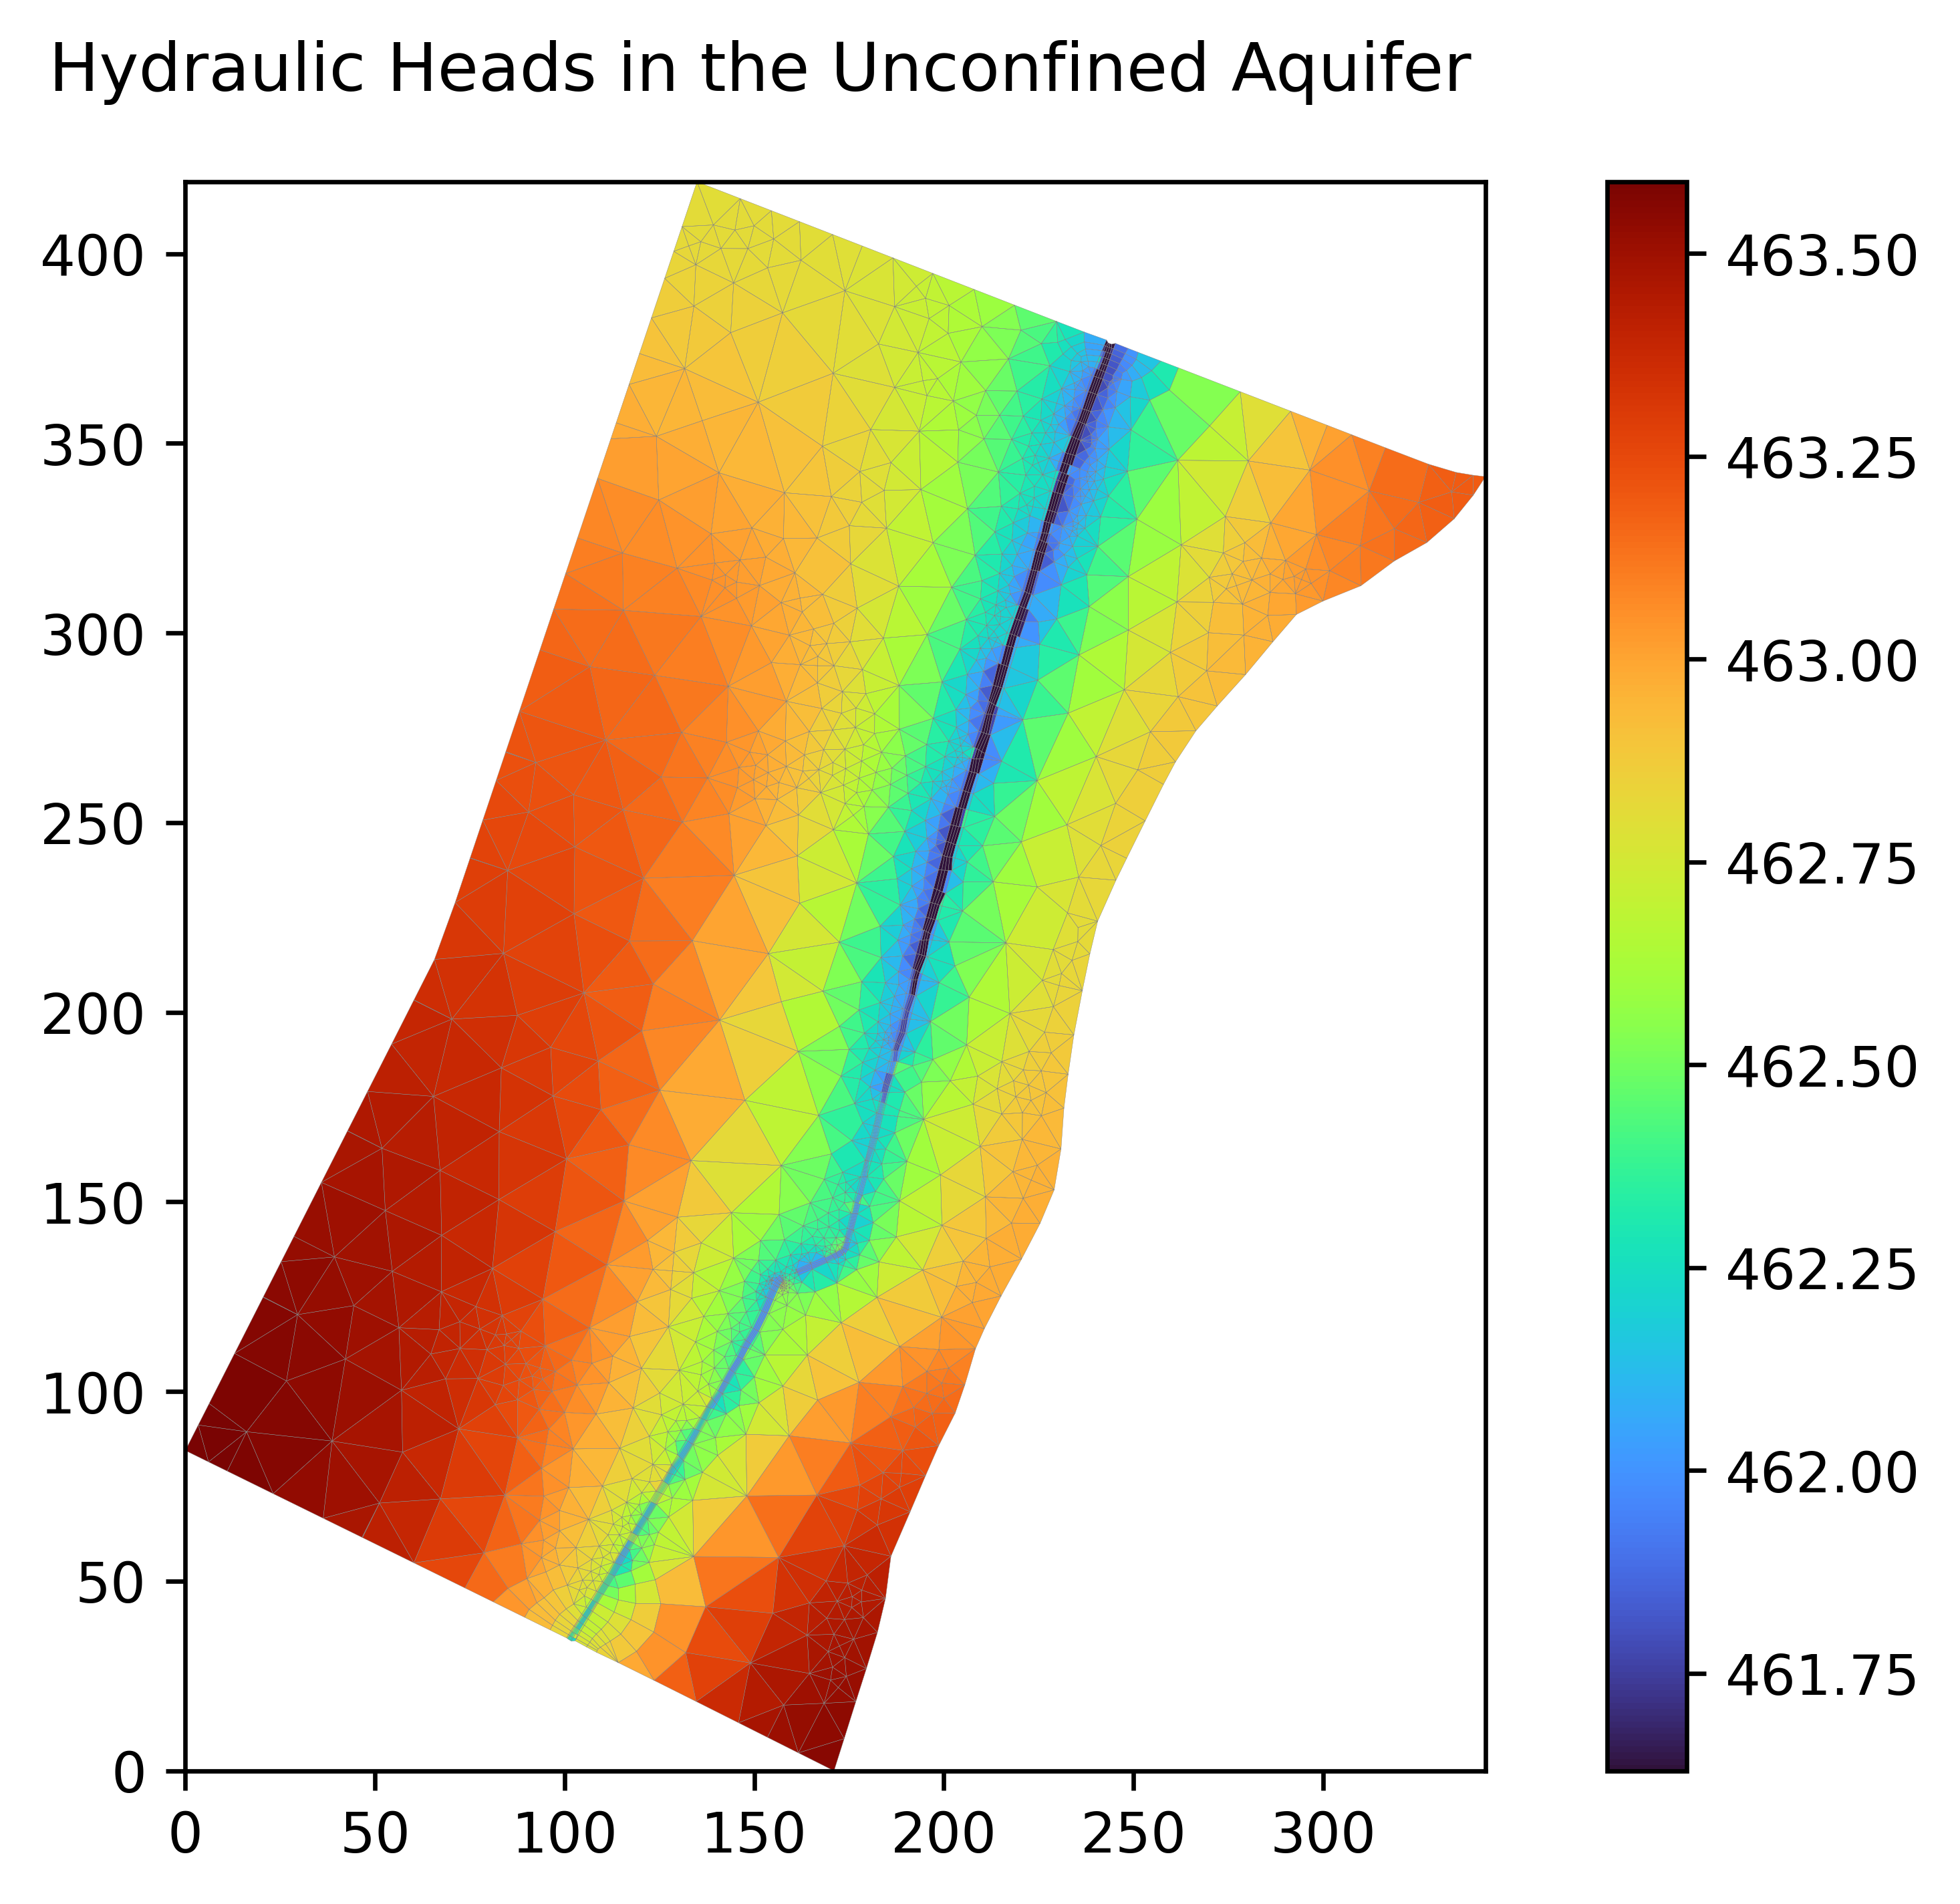
\includegraphics[width=\linewidth]{PICTURES/models_res/h_l1}
\endminipage\hfill
\minipage{0.32\textwidth}
  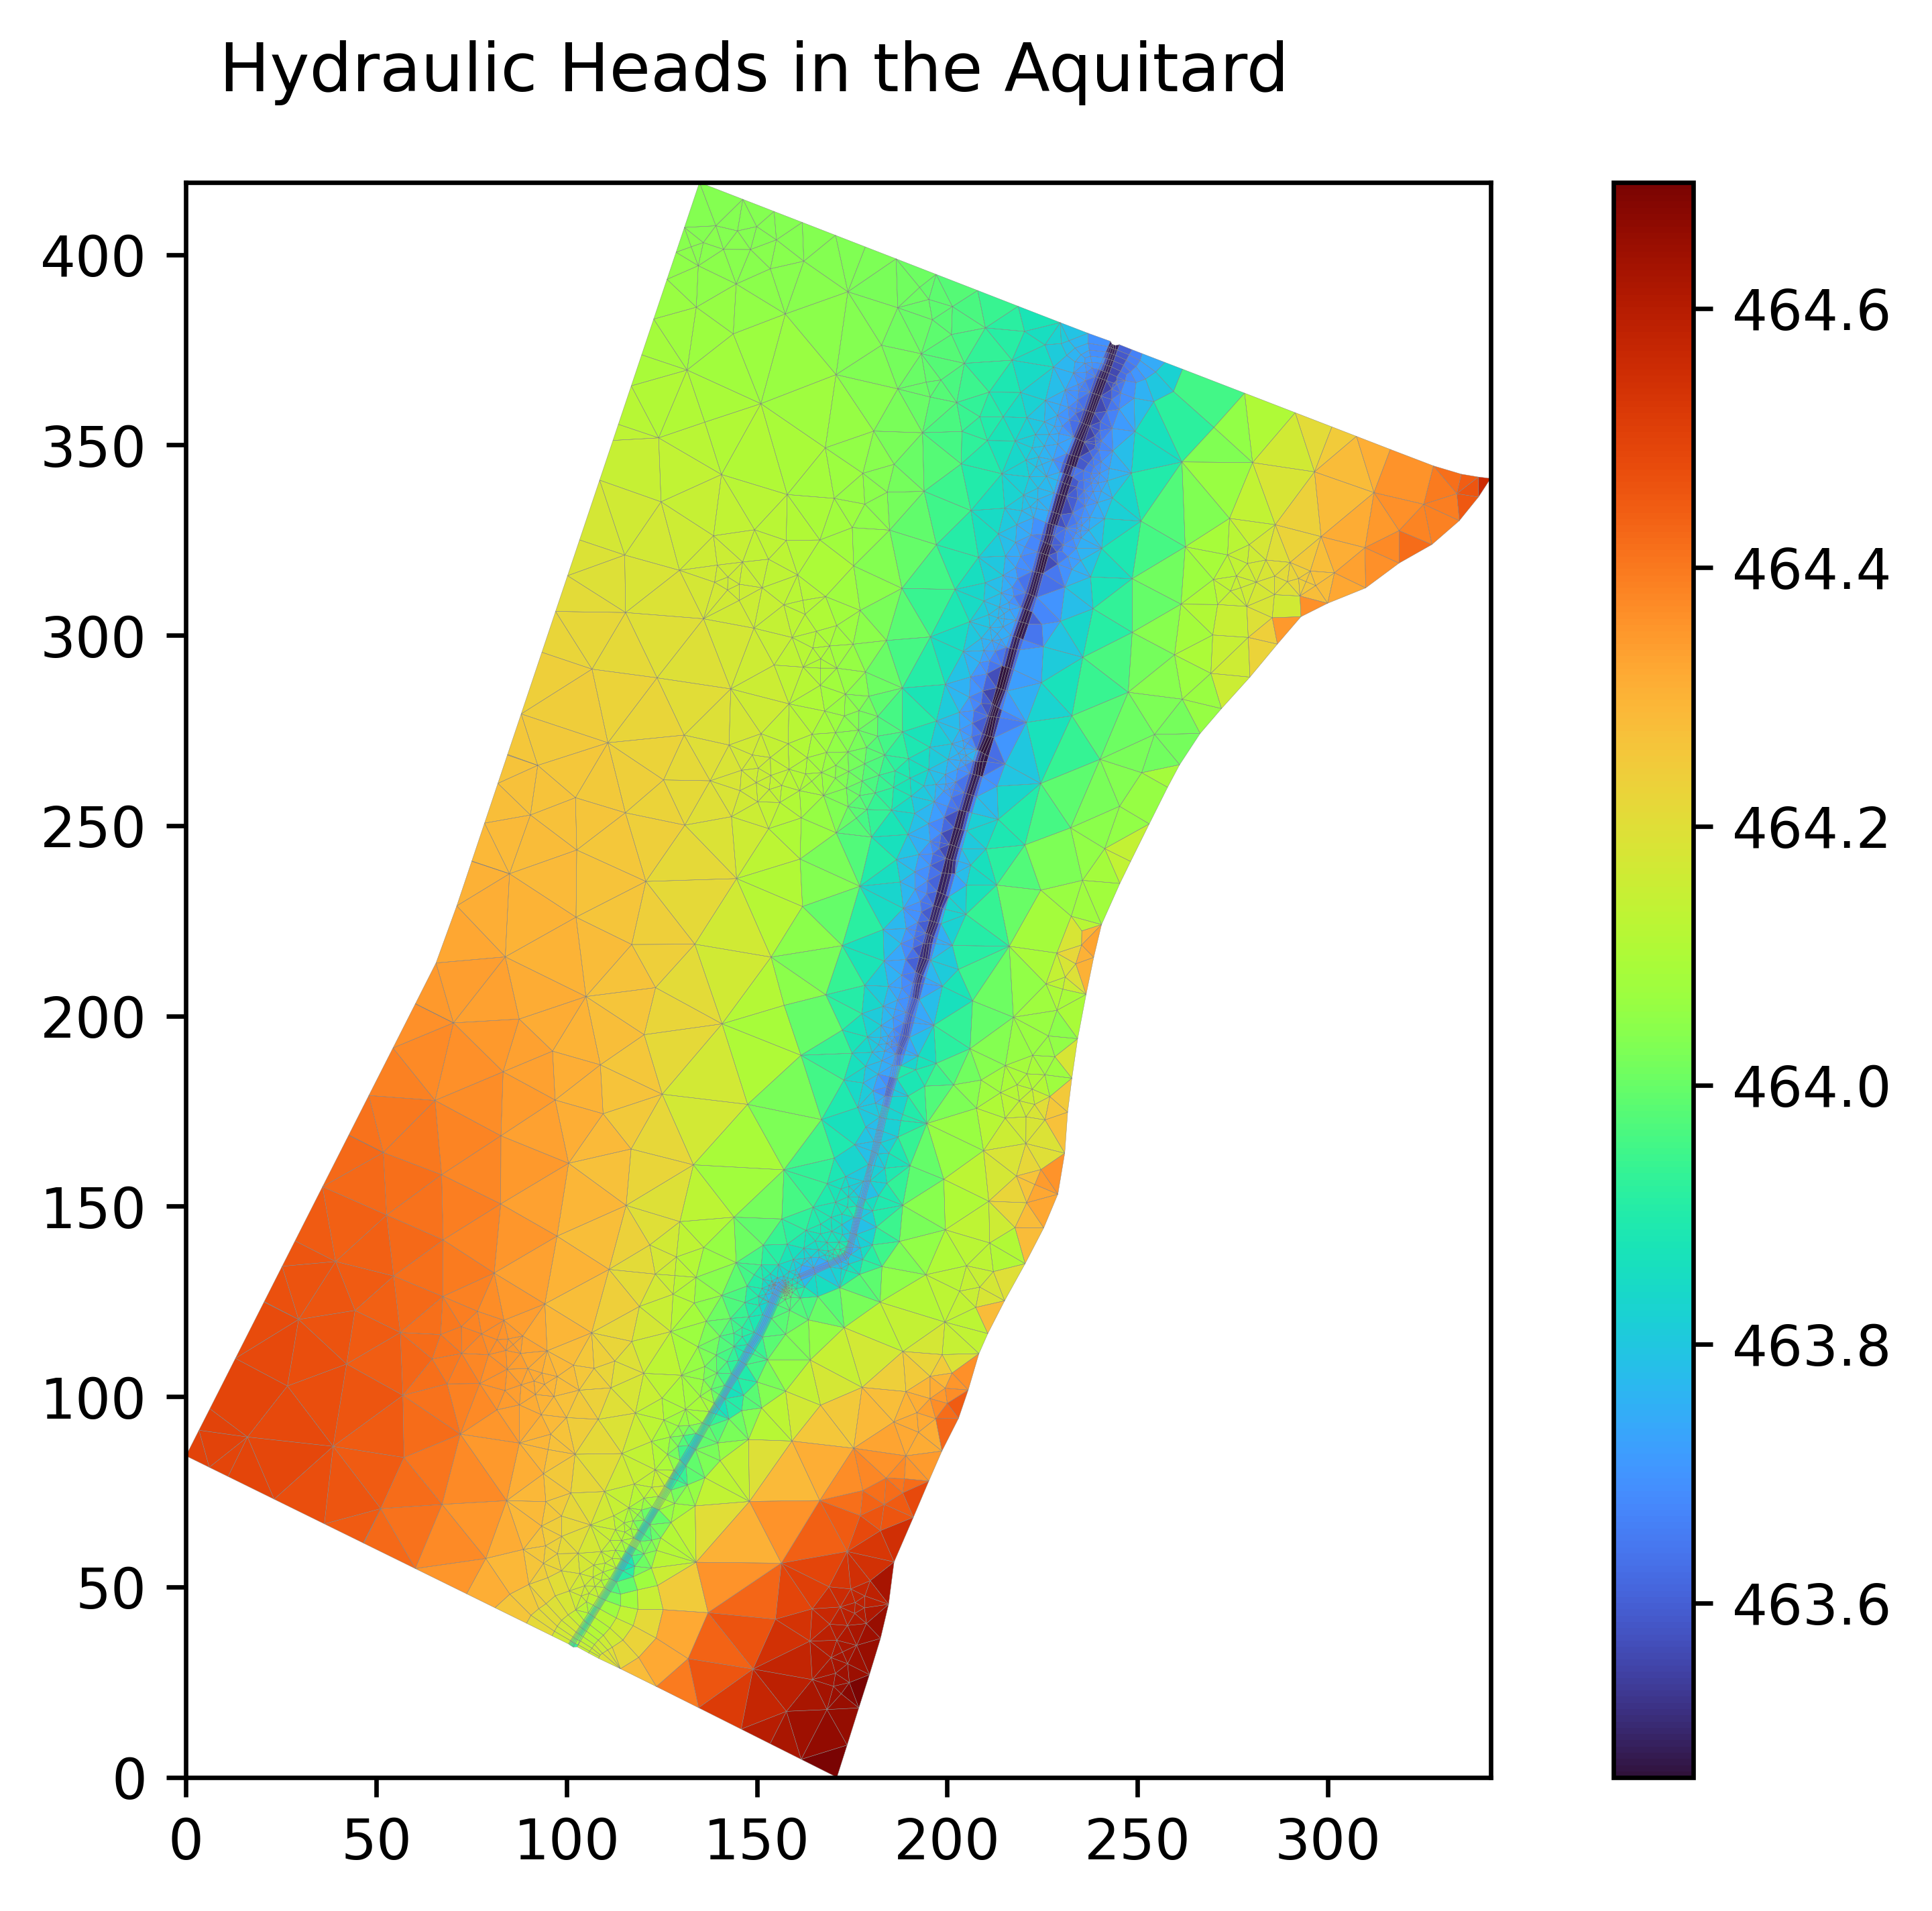
\includegraphics[width=\linewidth]{PICTURES/models_res/h_l2}
\endminipage\hfill
\minipage{0.32\textwidth}
  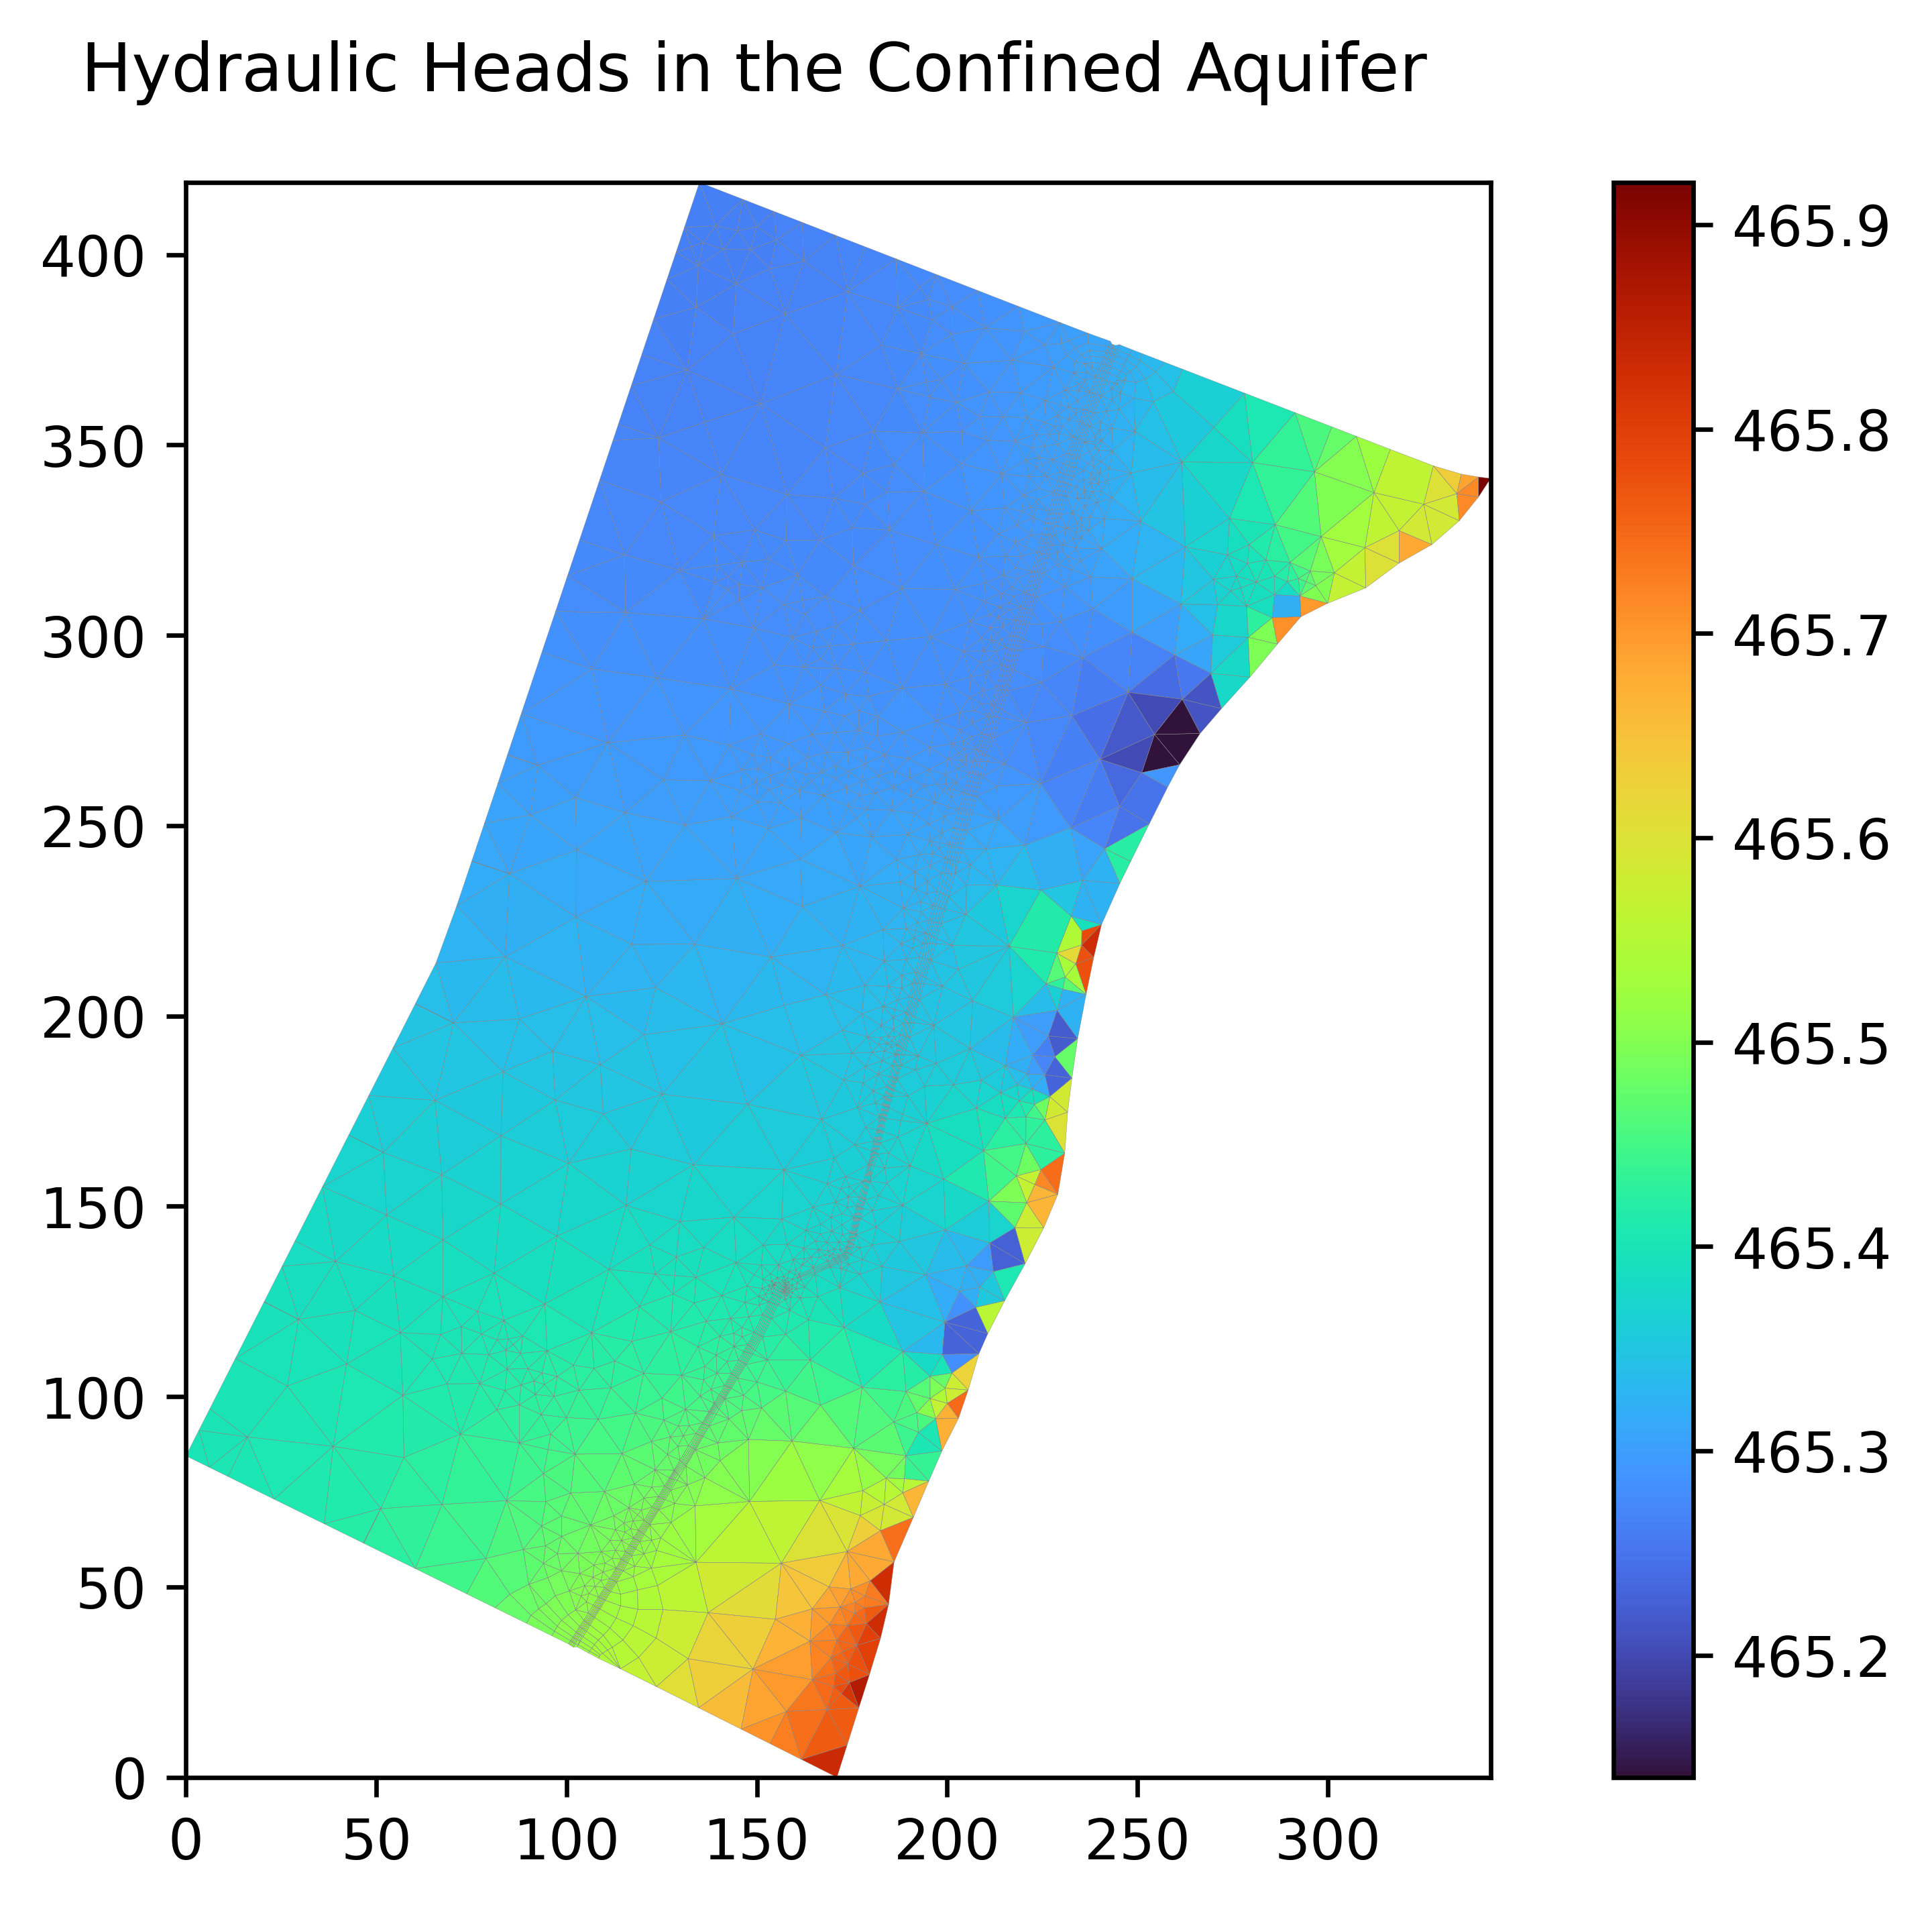
\includegraphics[width=\linewidth]{PICTURES/models_res/h_l3}
\endminipage
\caption{Starting heads in the GW Model.}\label{fig:mf6_res}
\end{figure}

\begin{figure}[H]
\minipage{0.5\textwidth}
  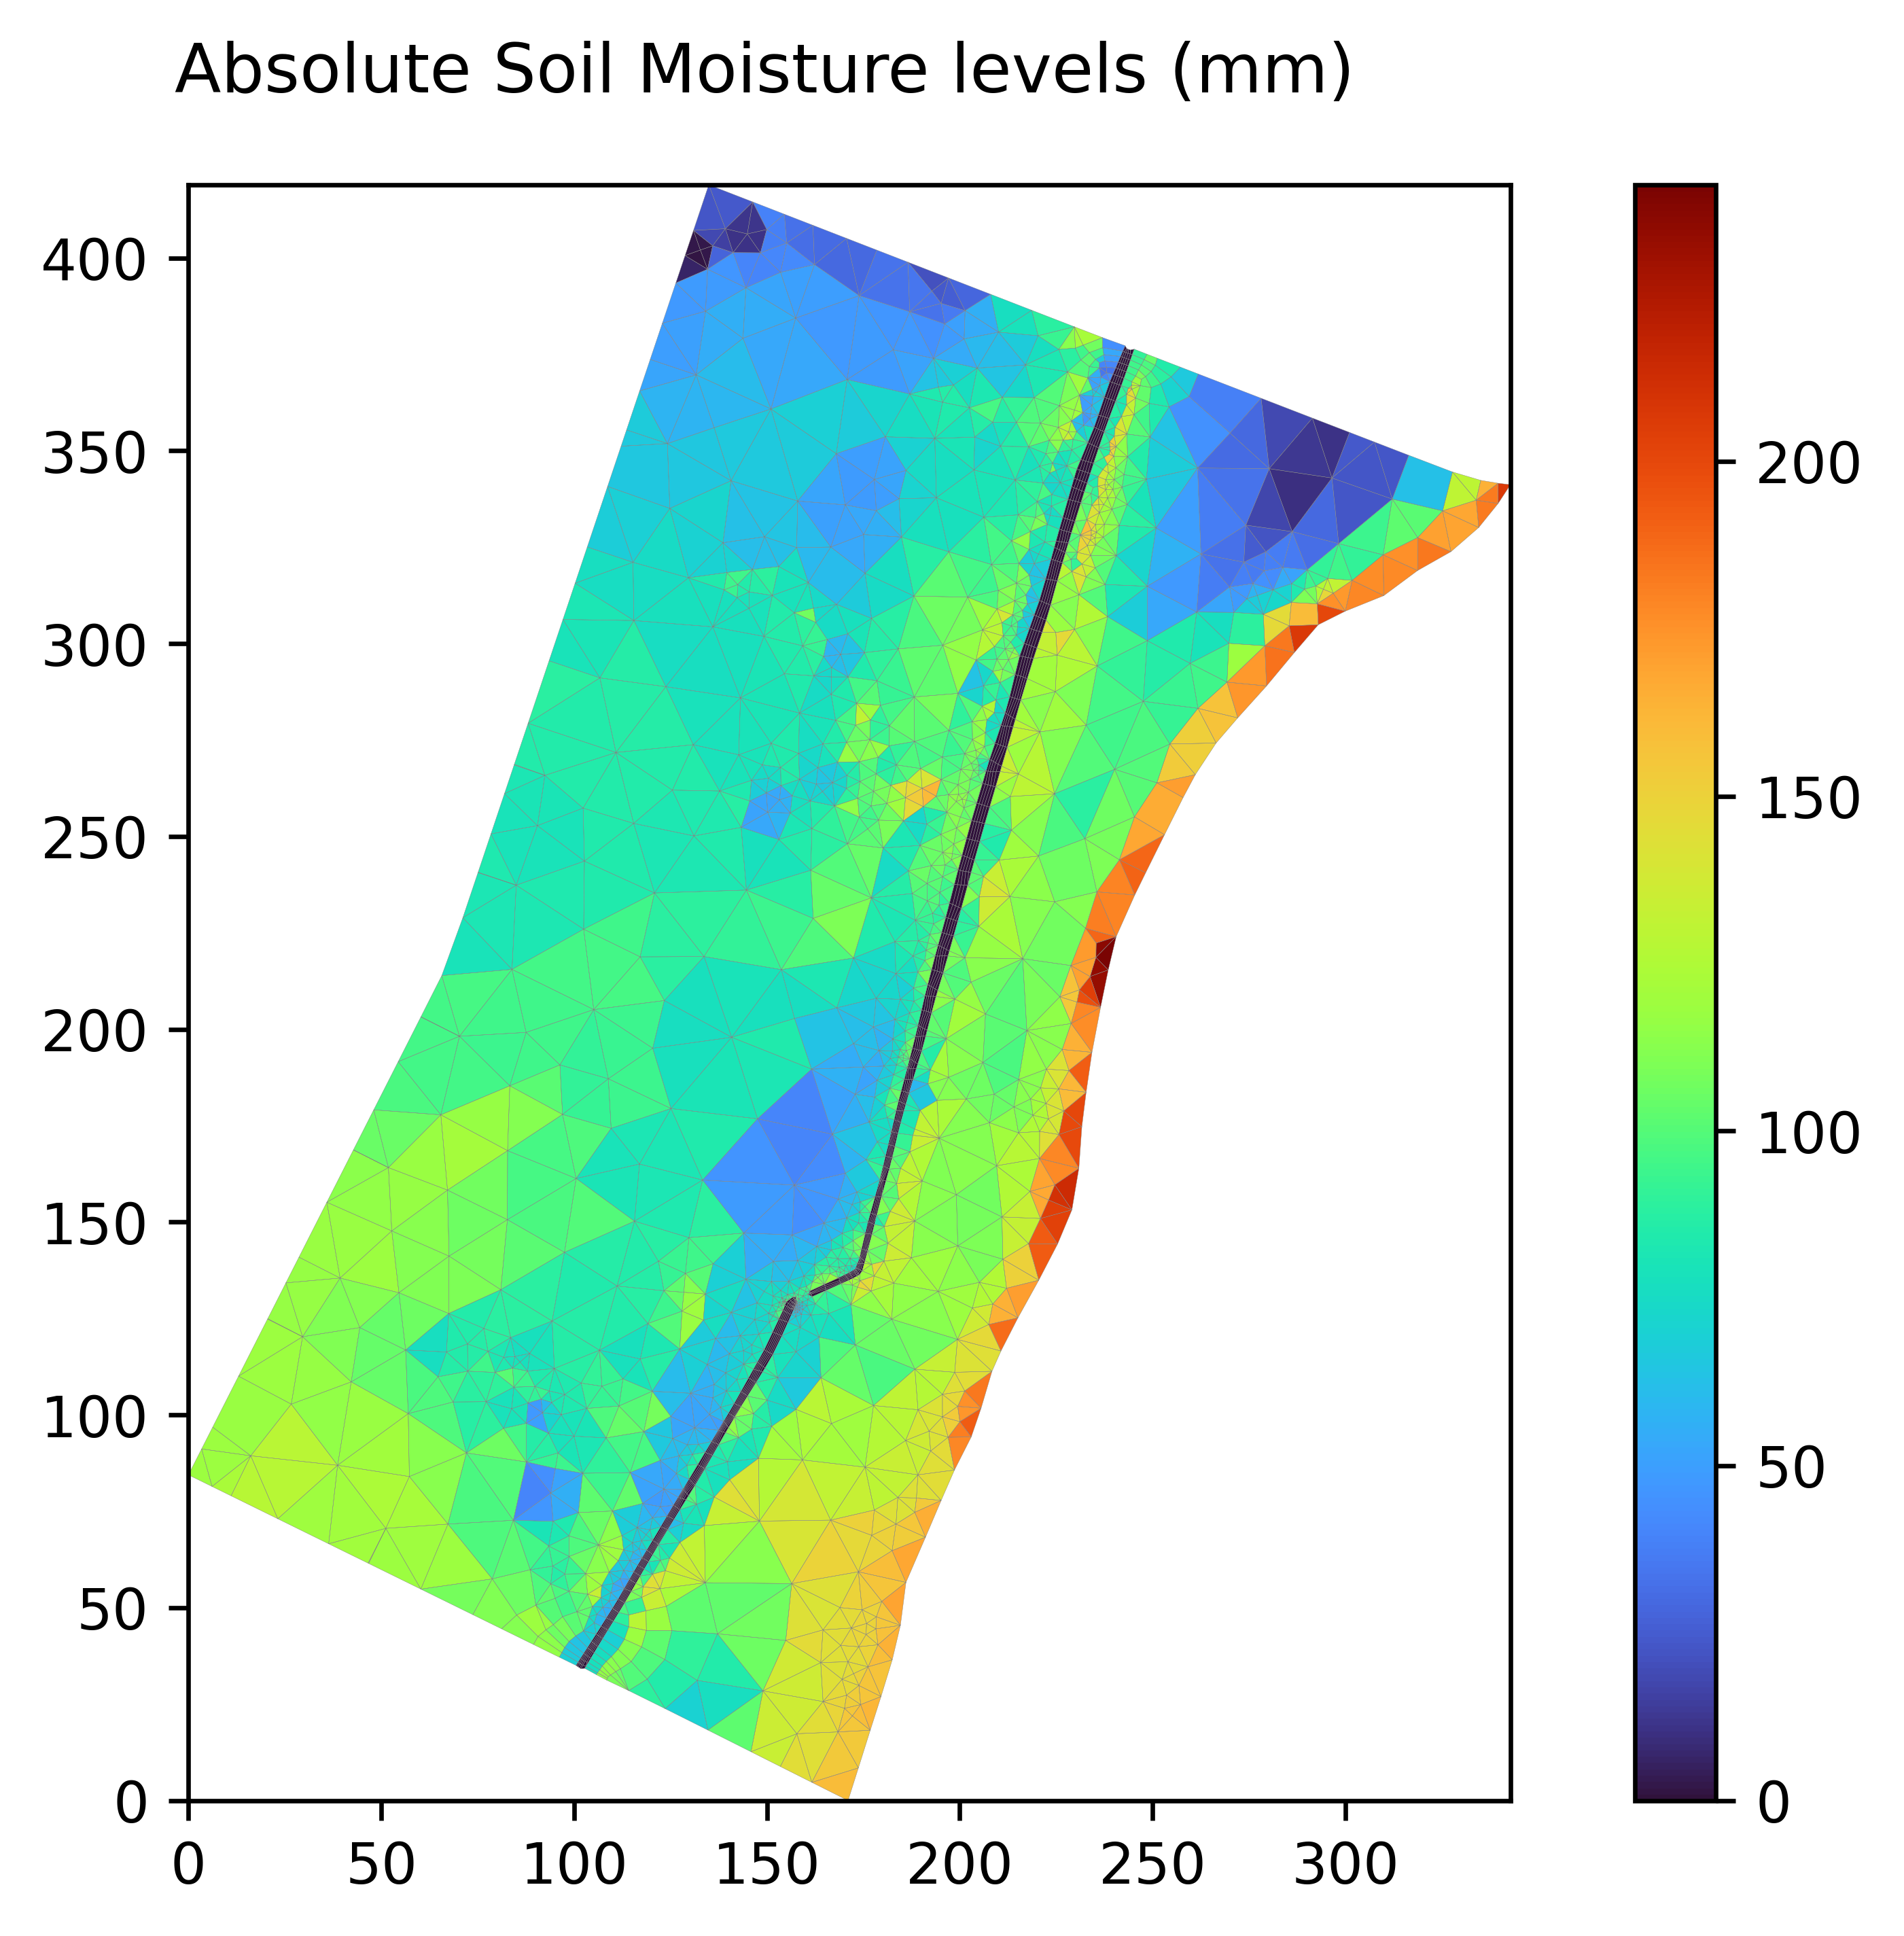
\includegraphics[width=0.9\linewidth]{PICTURES/models_res/sm_res}
\endminipage\hfill
\minipage{0.5\textwidth}
  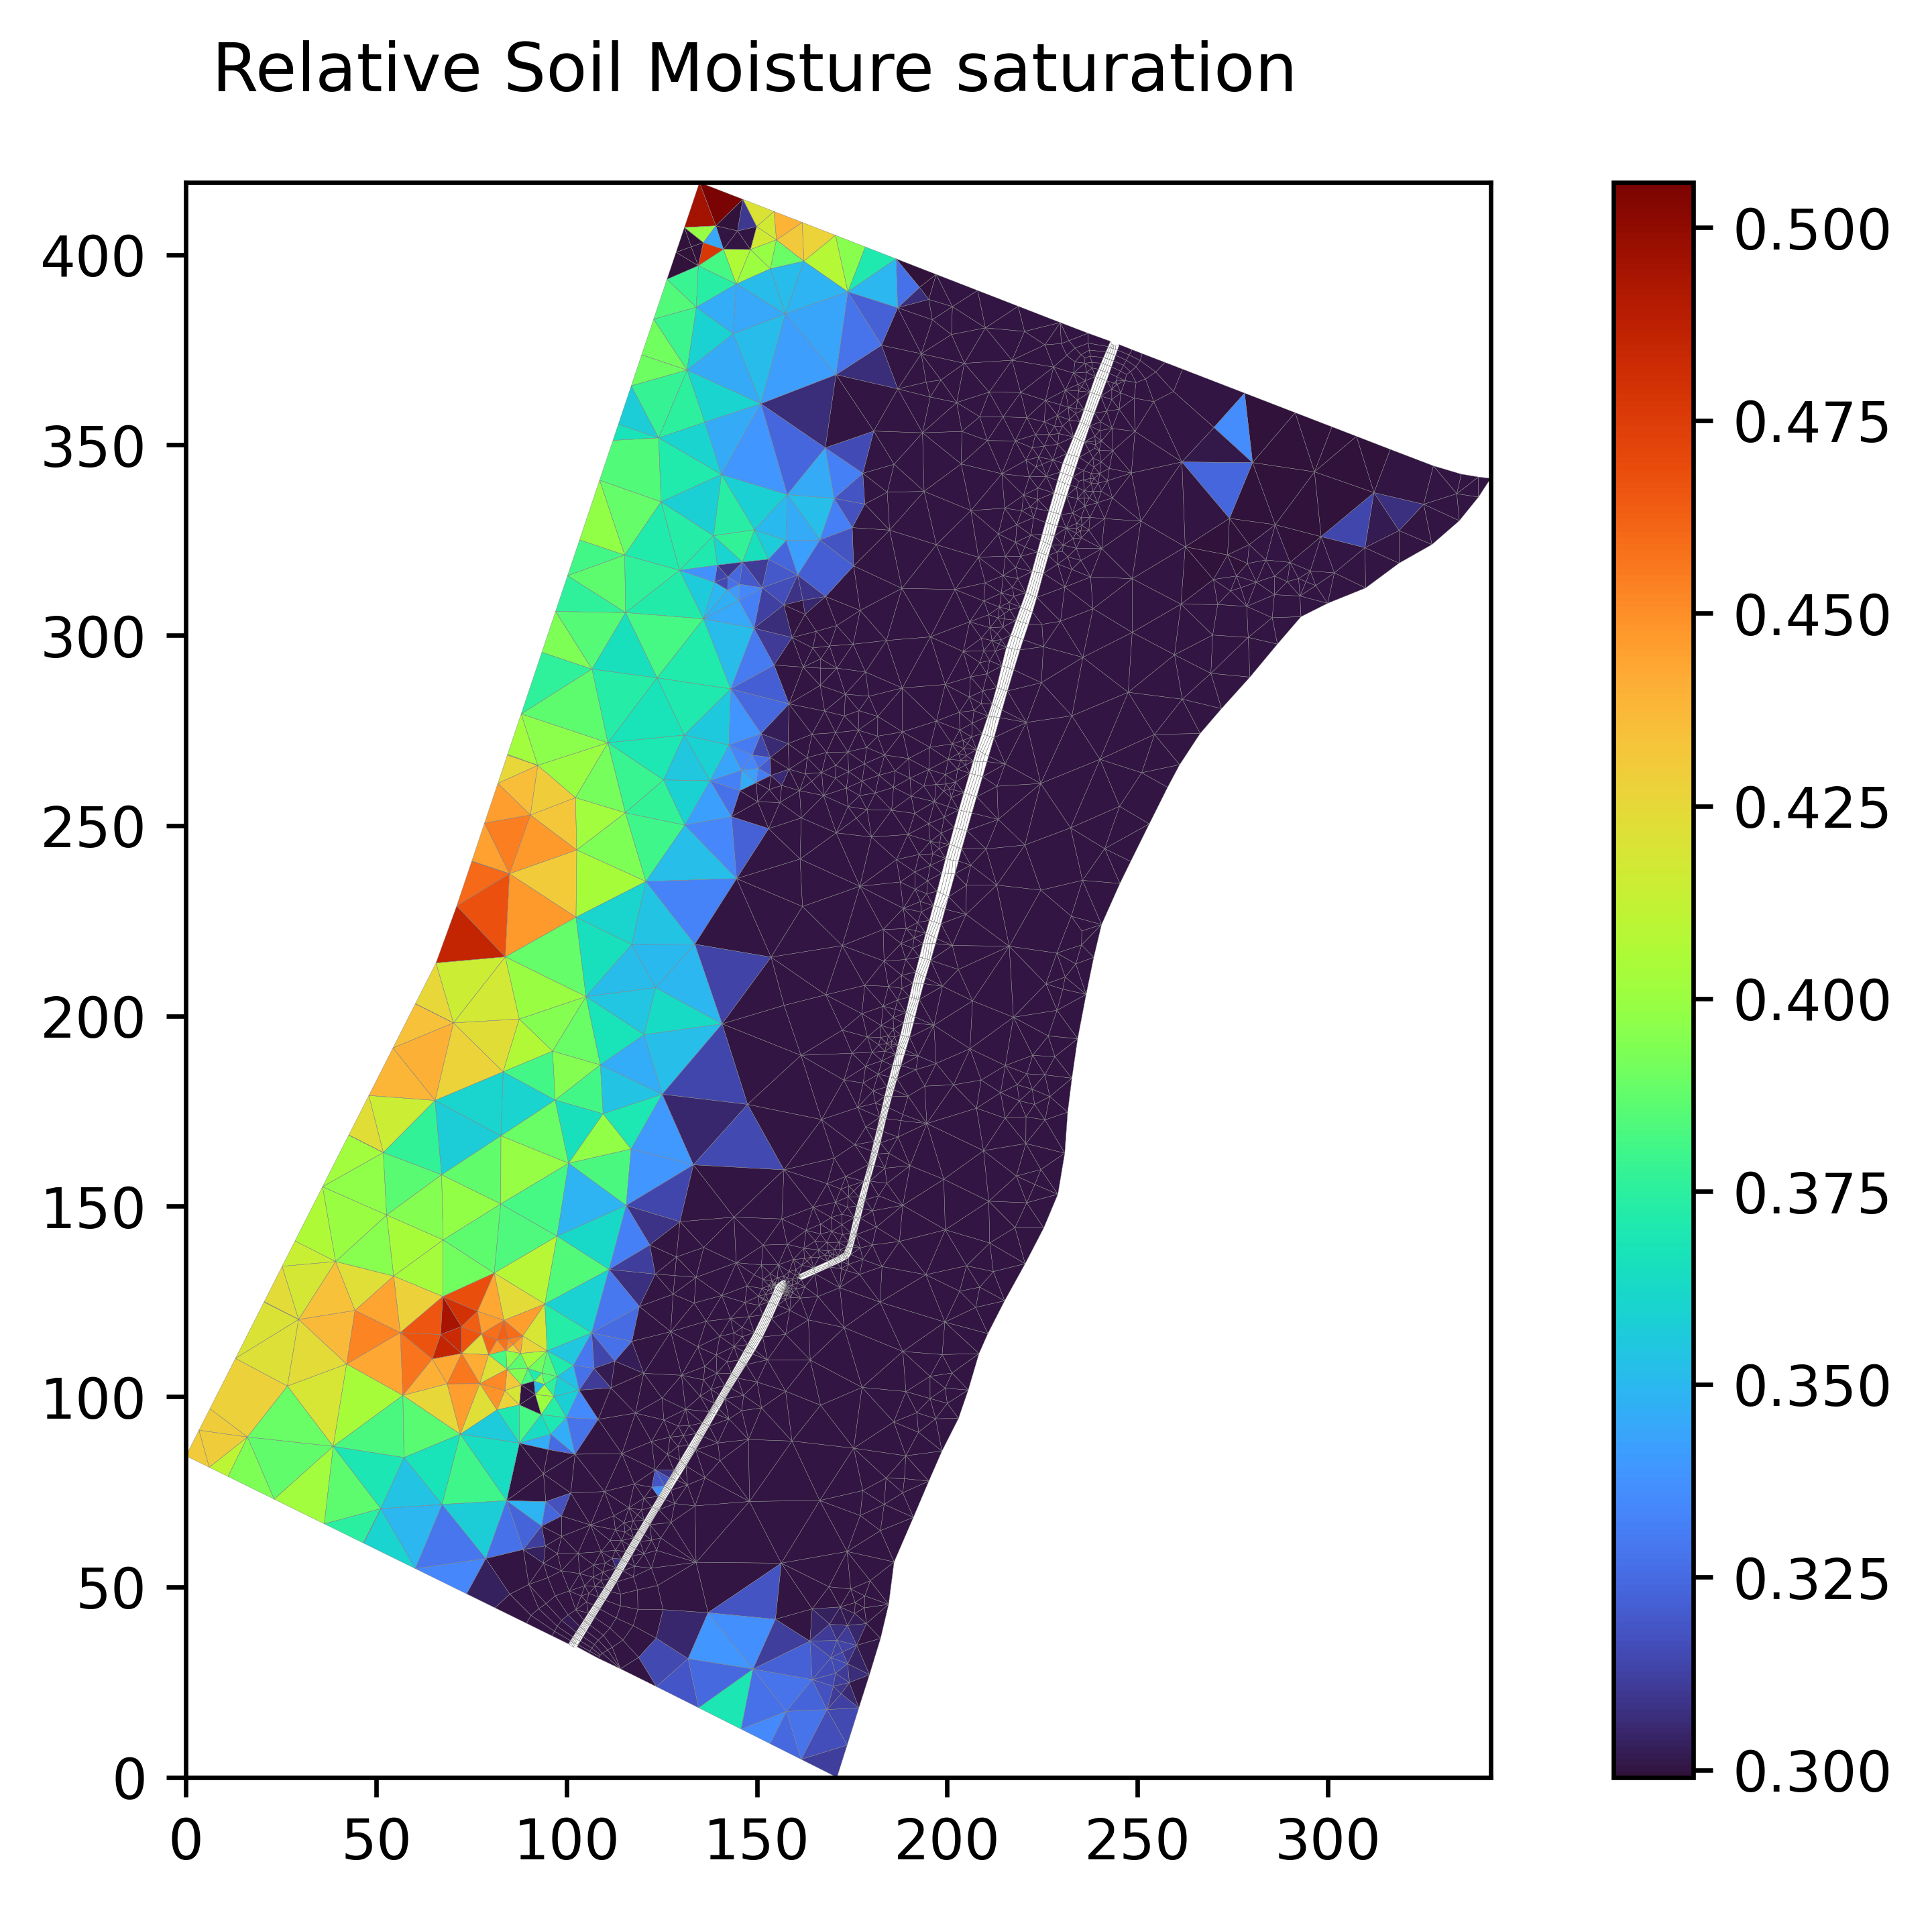
\includegraphics[width=0.9\linewidth]{PICTURES/models_res/sm_res_ratio}
\endminipage\hfill
\caption{Soil Moisture: left - absolute levels (mm); right - relative saturation.}\label{fig:sm_res}
\end{figure}

\begin{figure}[H]
    \centering
    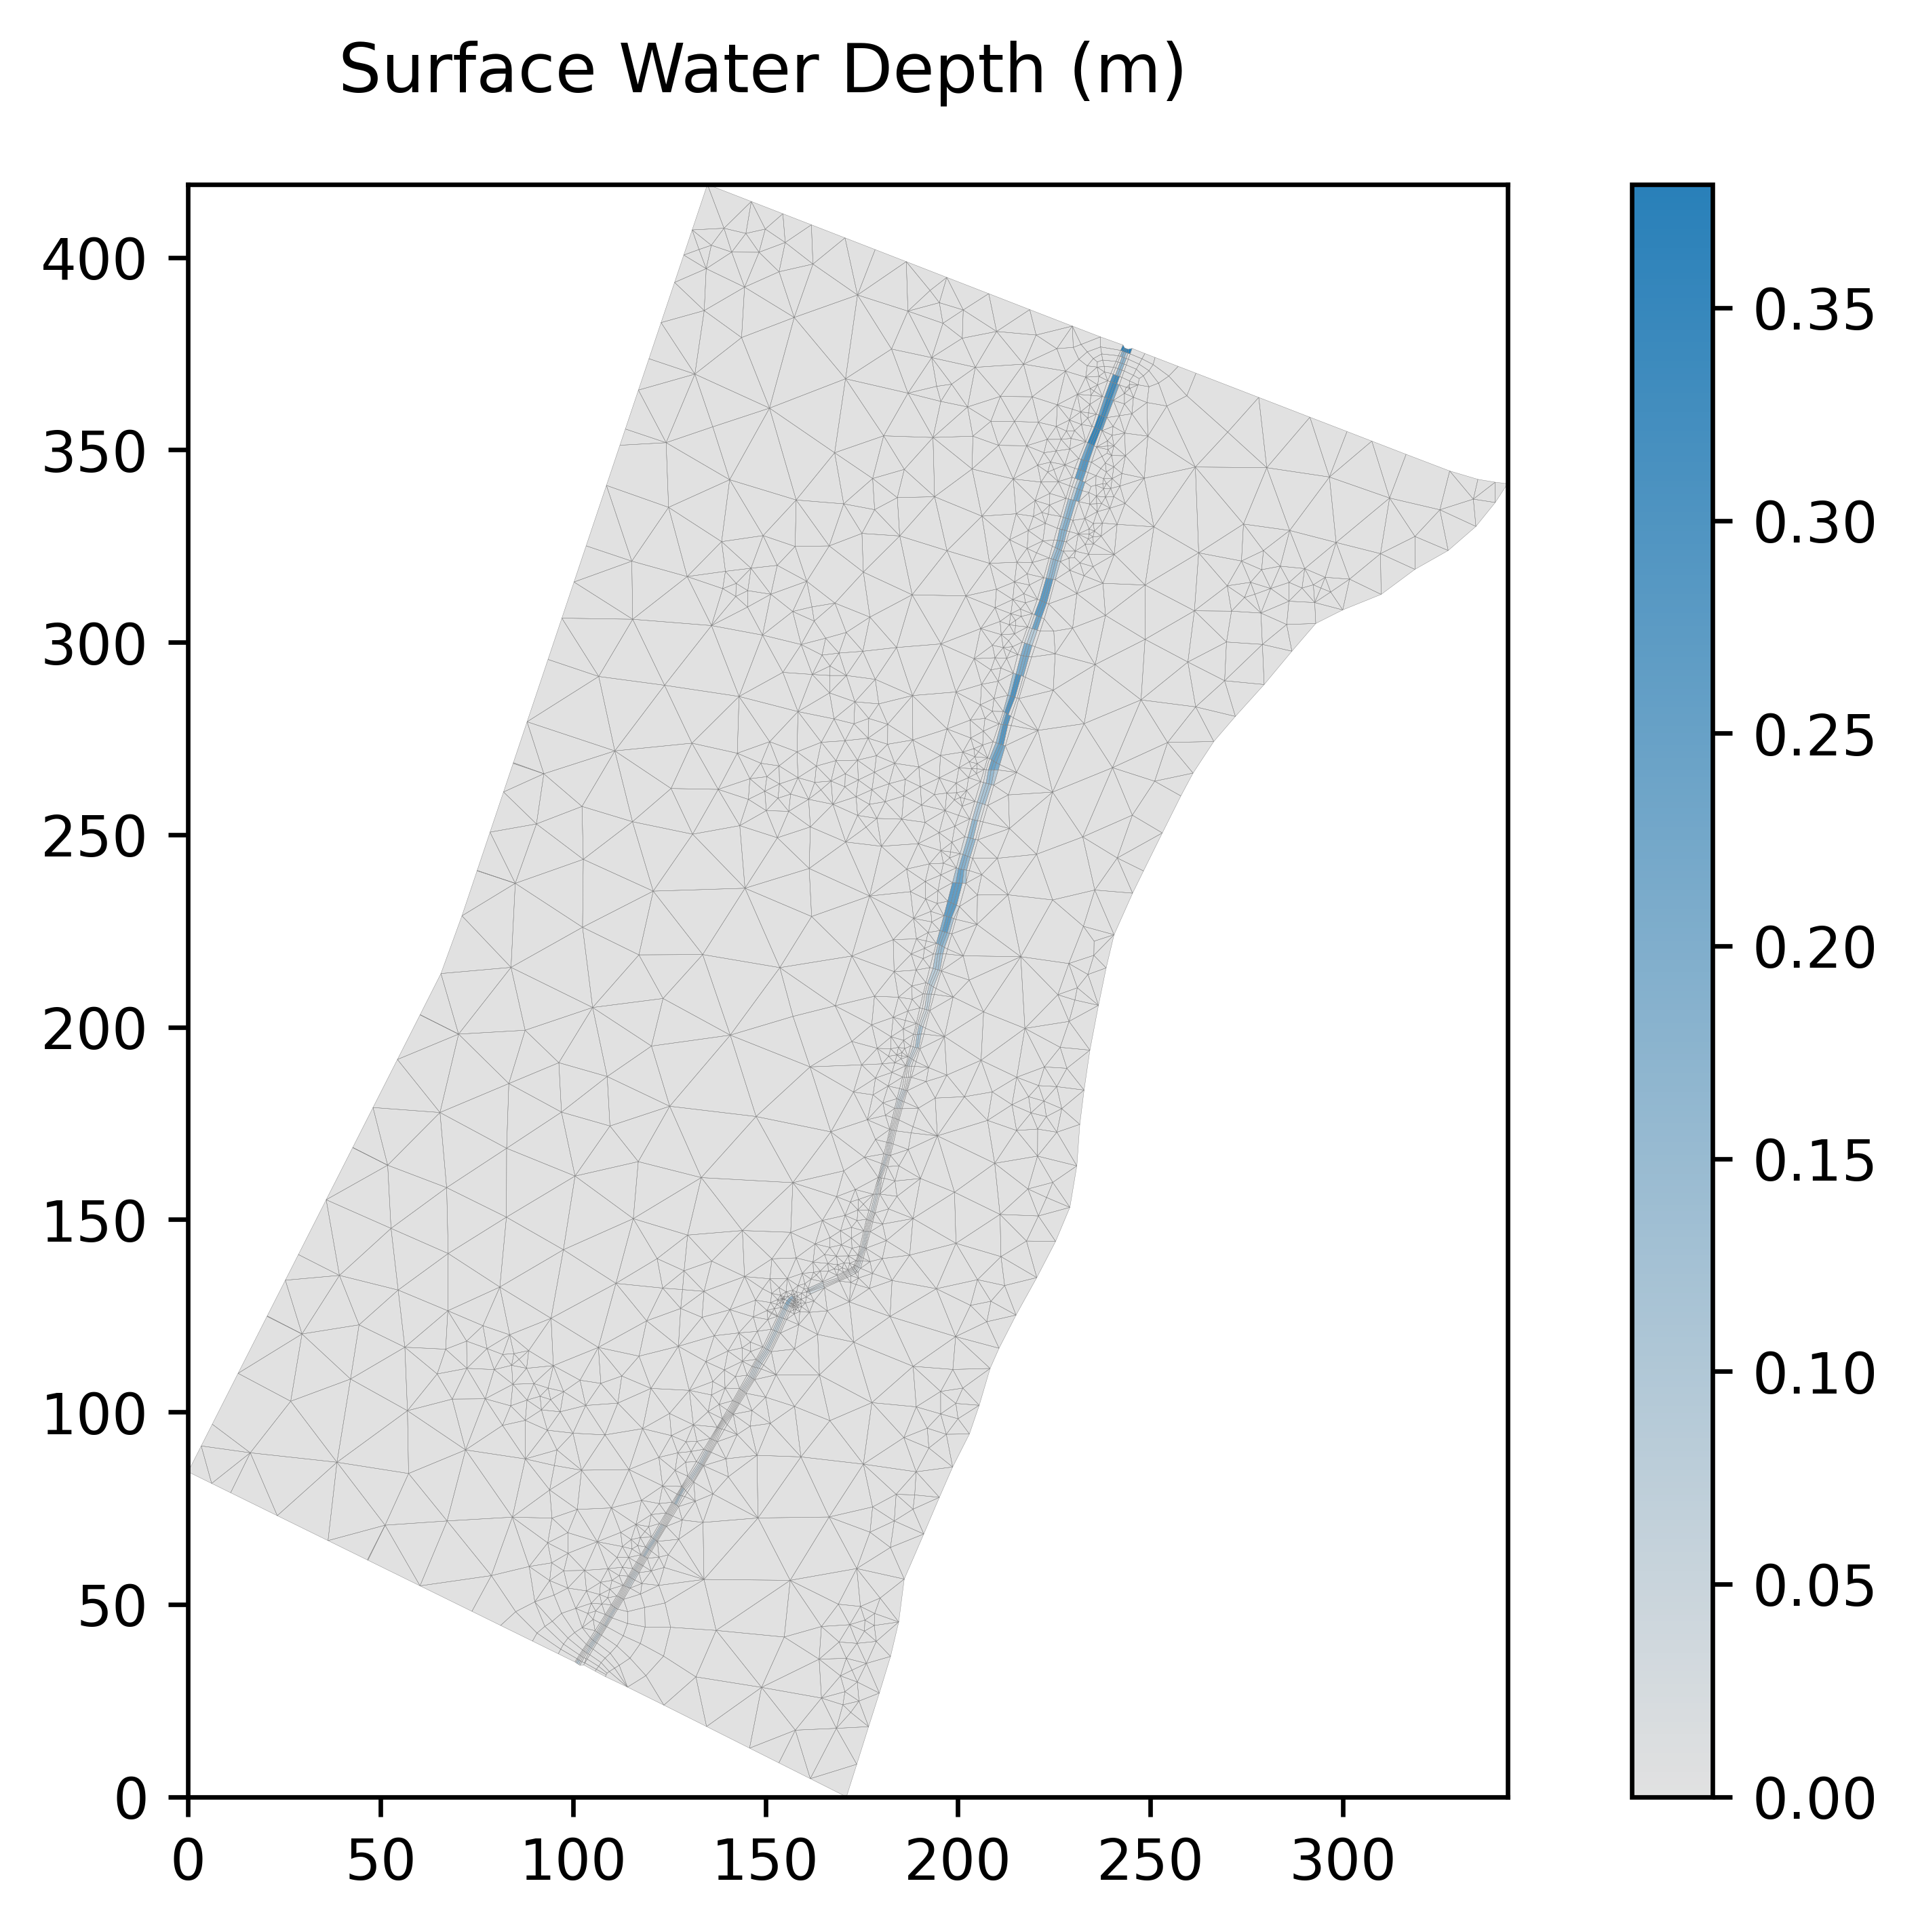
\includegraphics[scale=0.5]{PICTURES/models_res/sws}
    \caption{SW levels at the end of the simulation period.}
    \label{fig:sw_res}
\end{figure}



\section{Comparison with Measured Observations}
\label{obs}
The following plots compare the simulated and observed hydraulic heads at the observation locations as illustrated in \ref{fig:obs_pts}. It is observed that the simulated observations agree with the measured observations qualitatively in most locations. 

\begin{figure}[H]
    \centering
    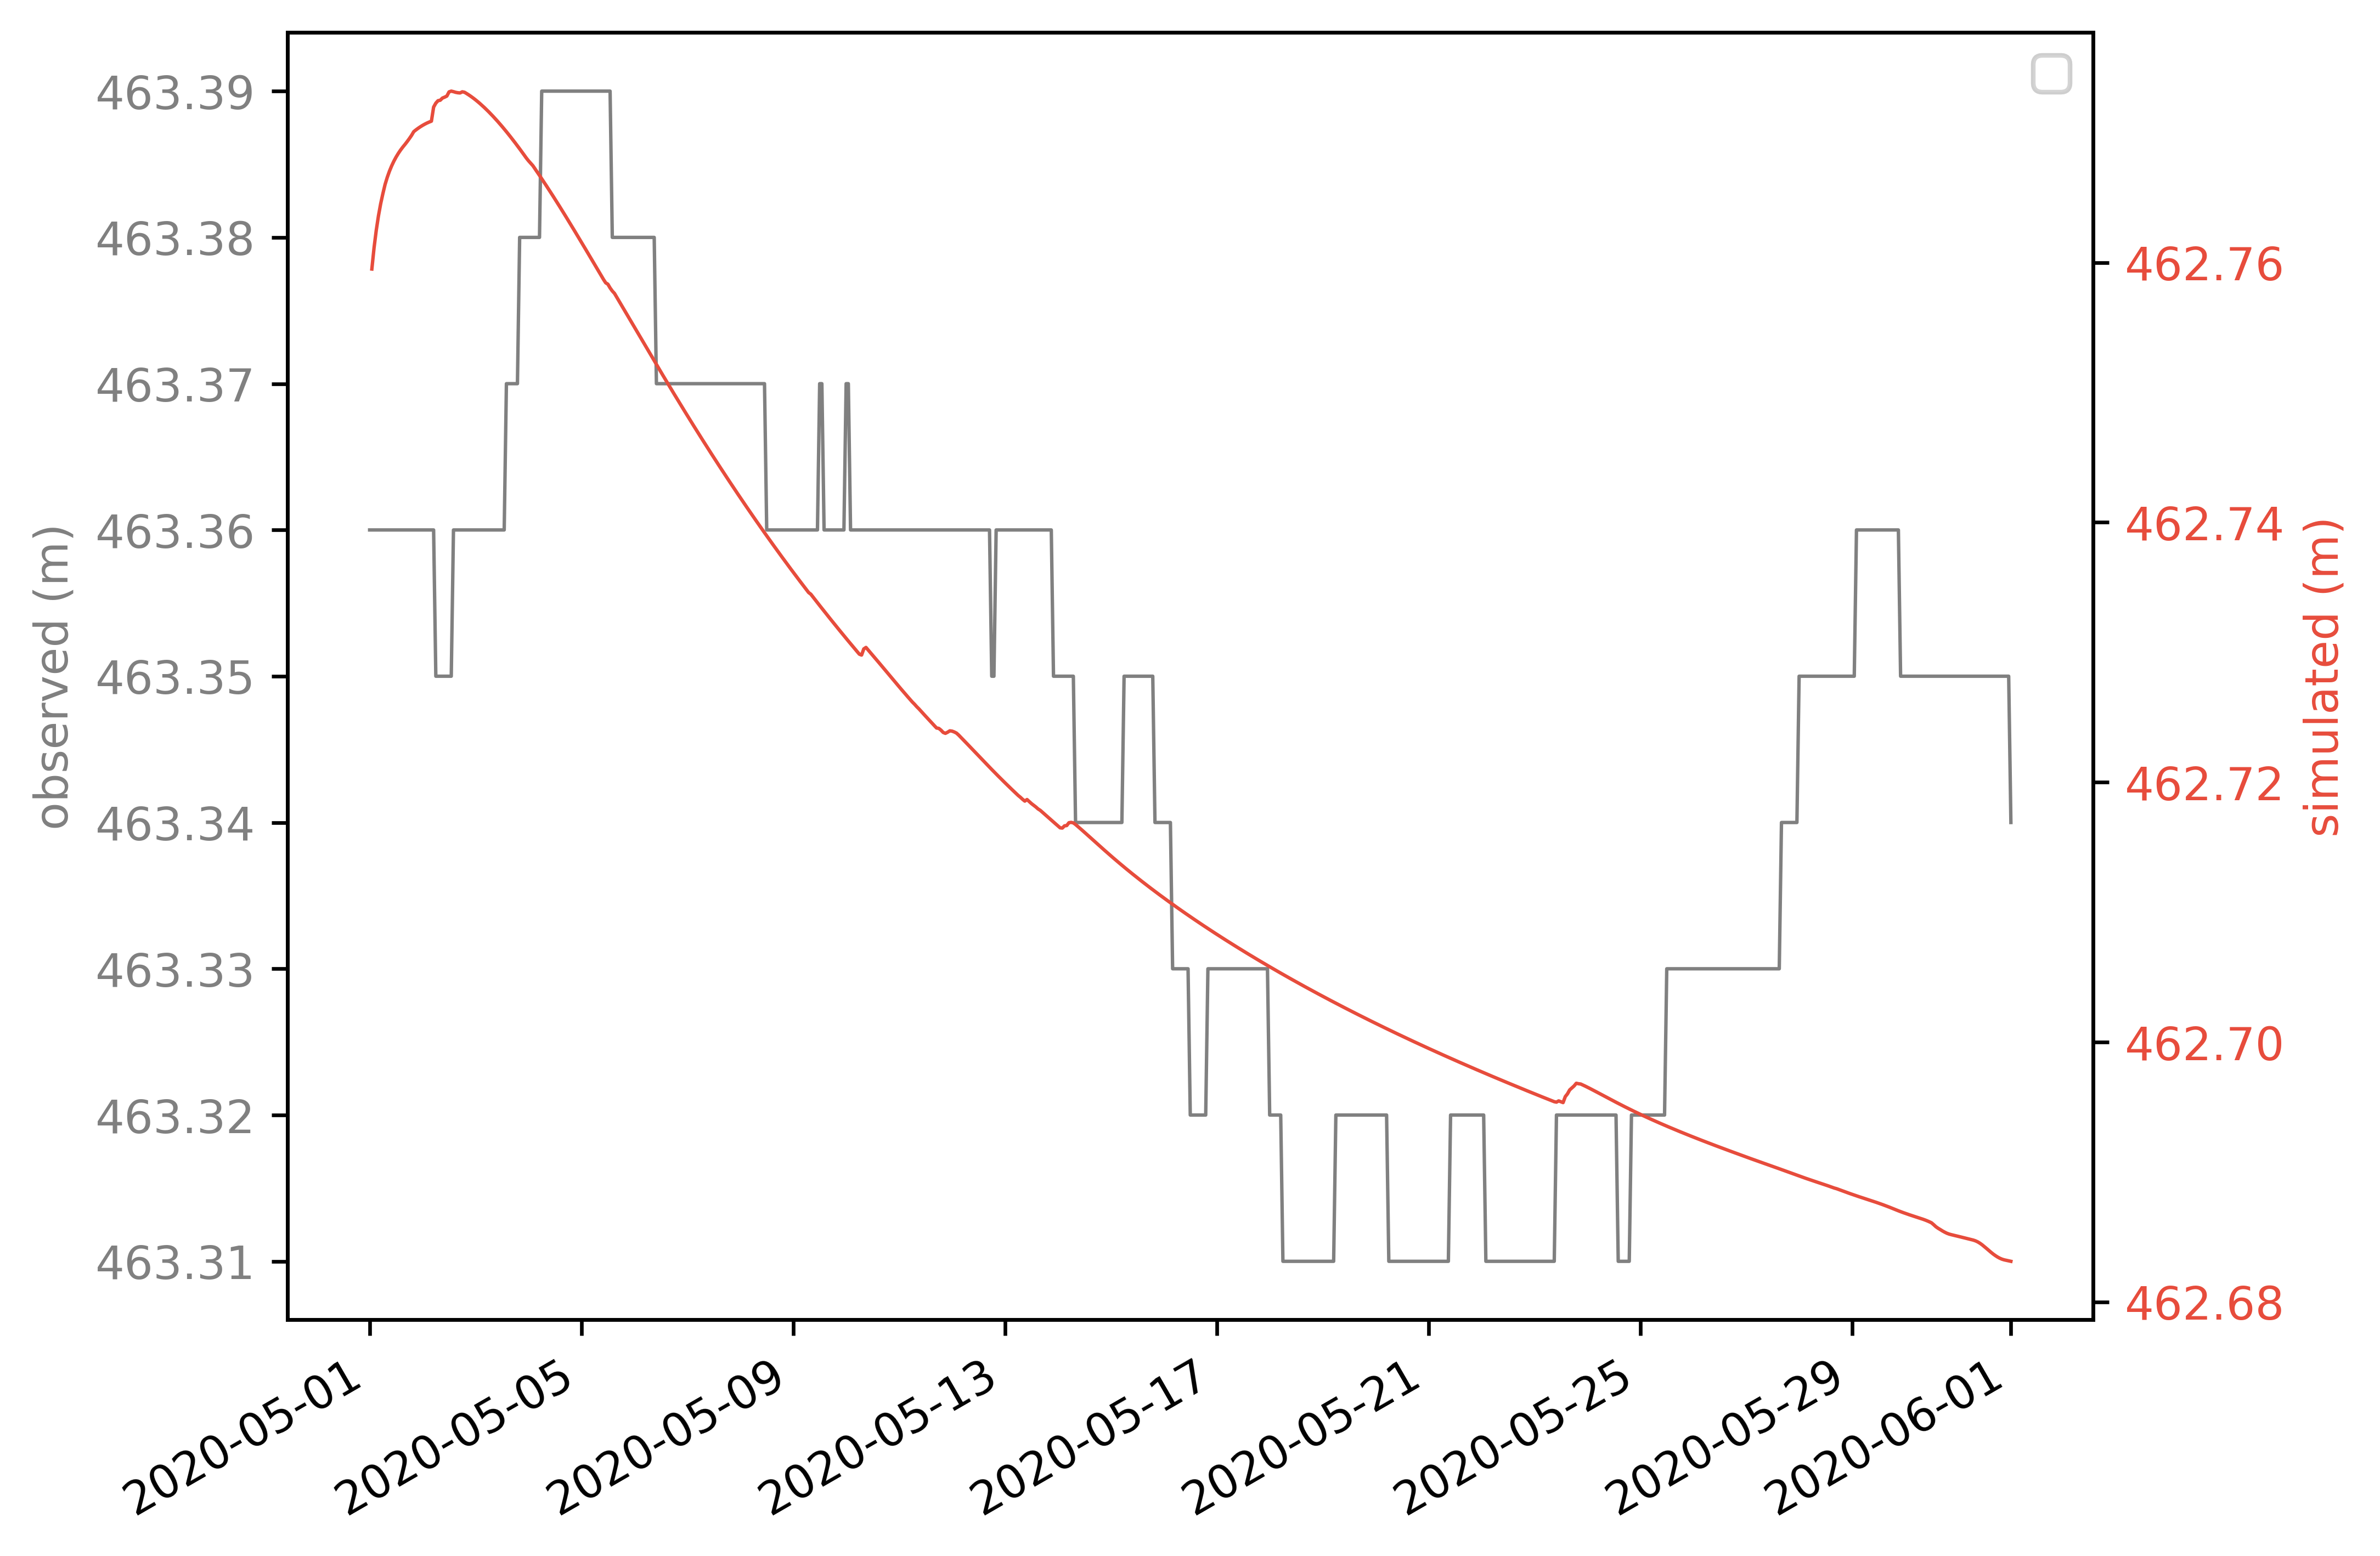
\includegraphics[width=\linewidth]{PICTURES/models_res/p2}
    \caption{Comparing simulated and measured observations at location P-2.}
    \label{fig:p2}
\end{figure}

\begin{figure}[H]
    \centering
    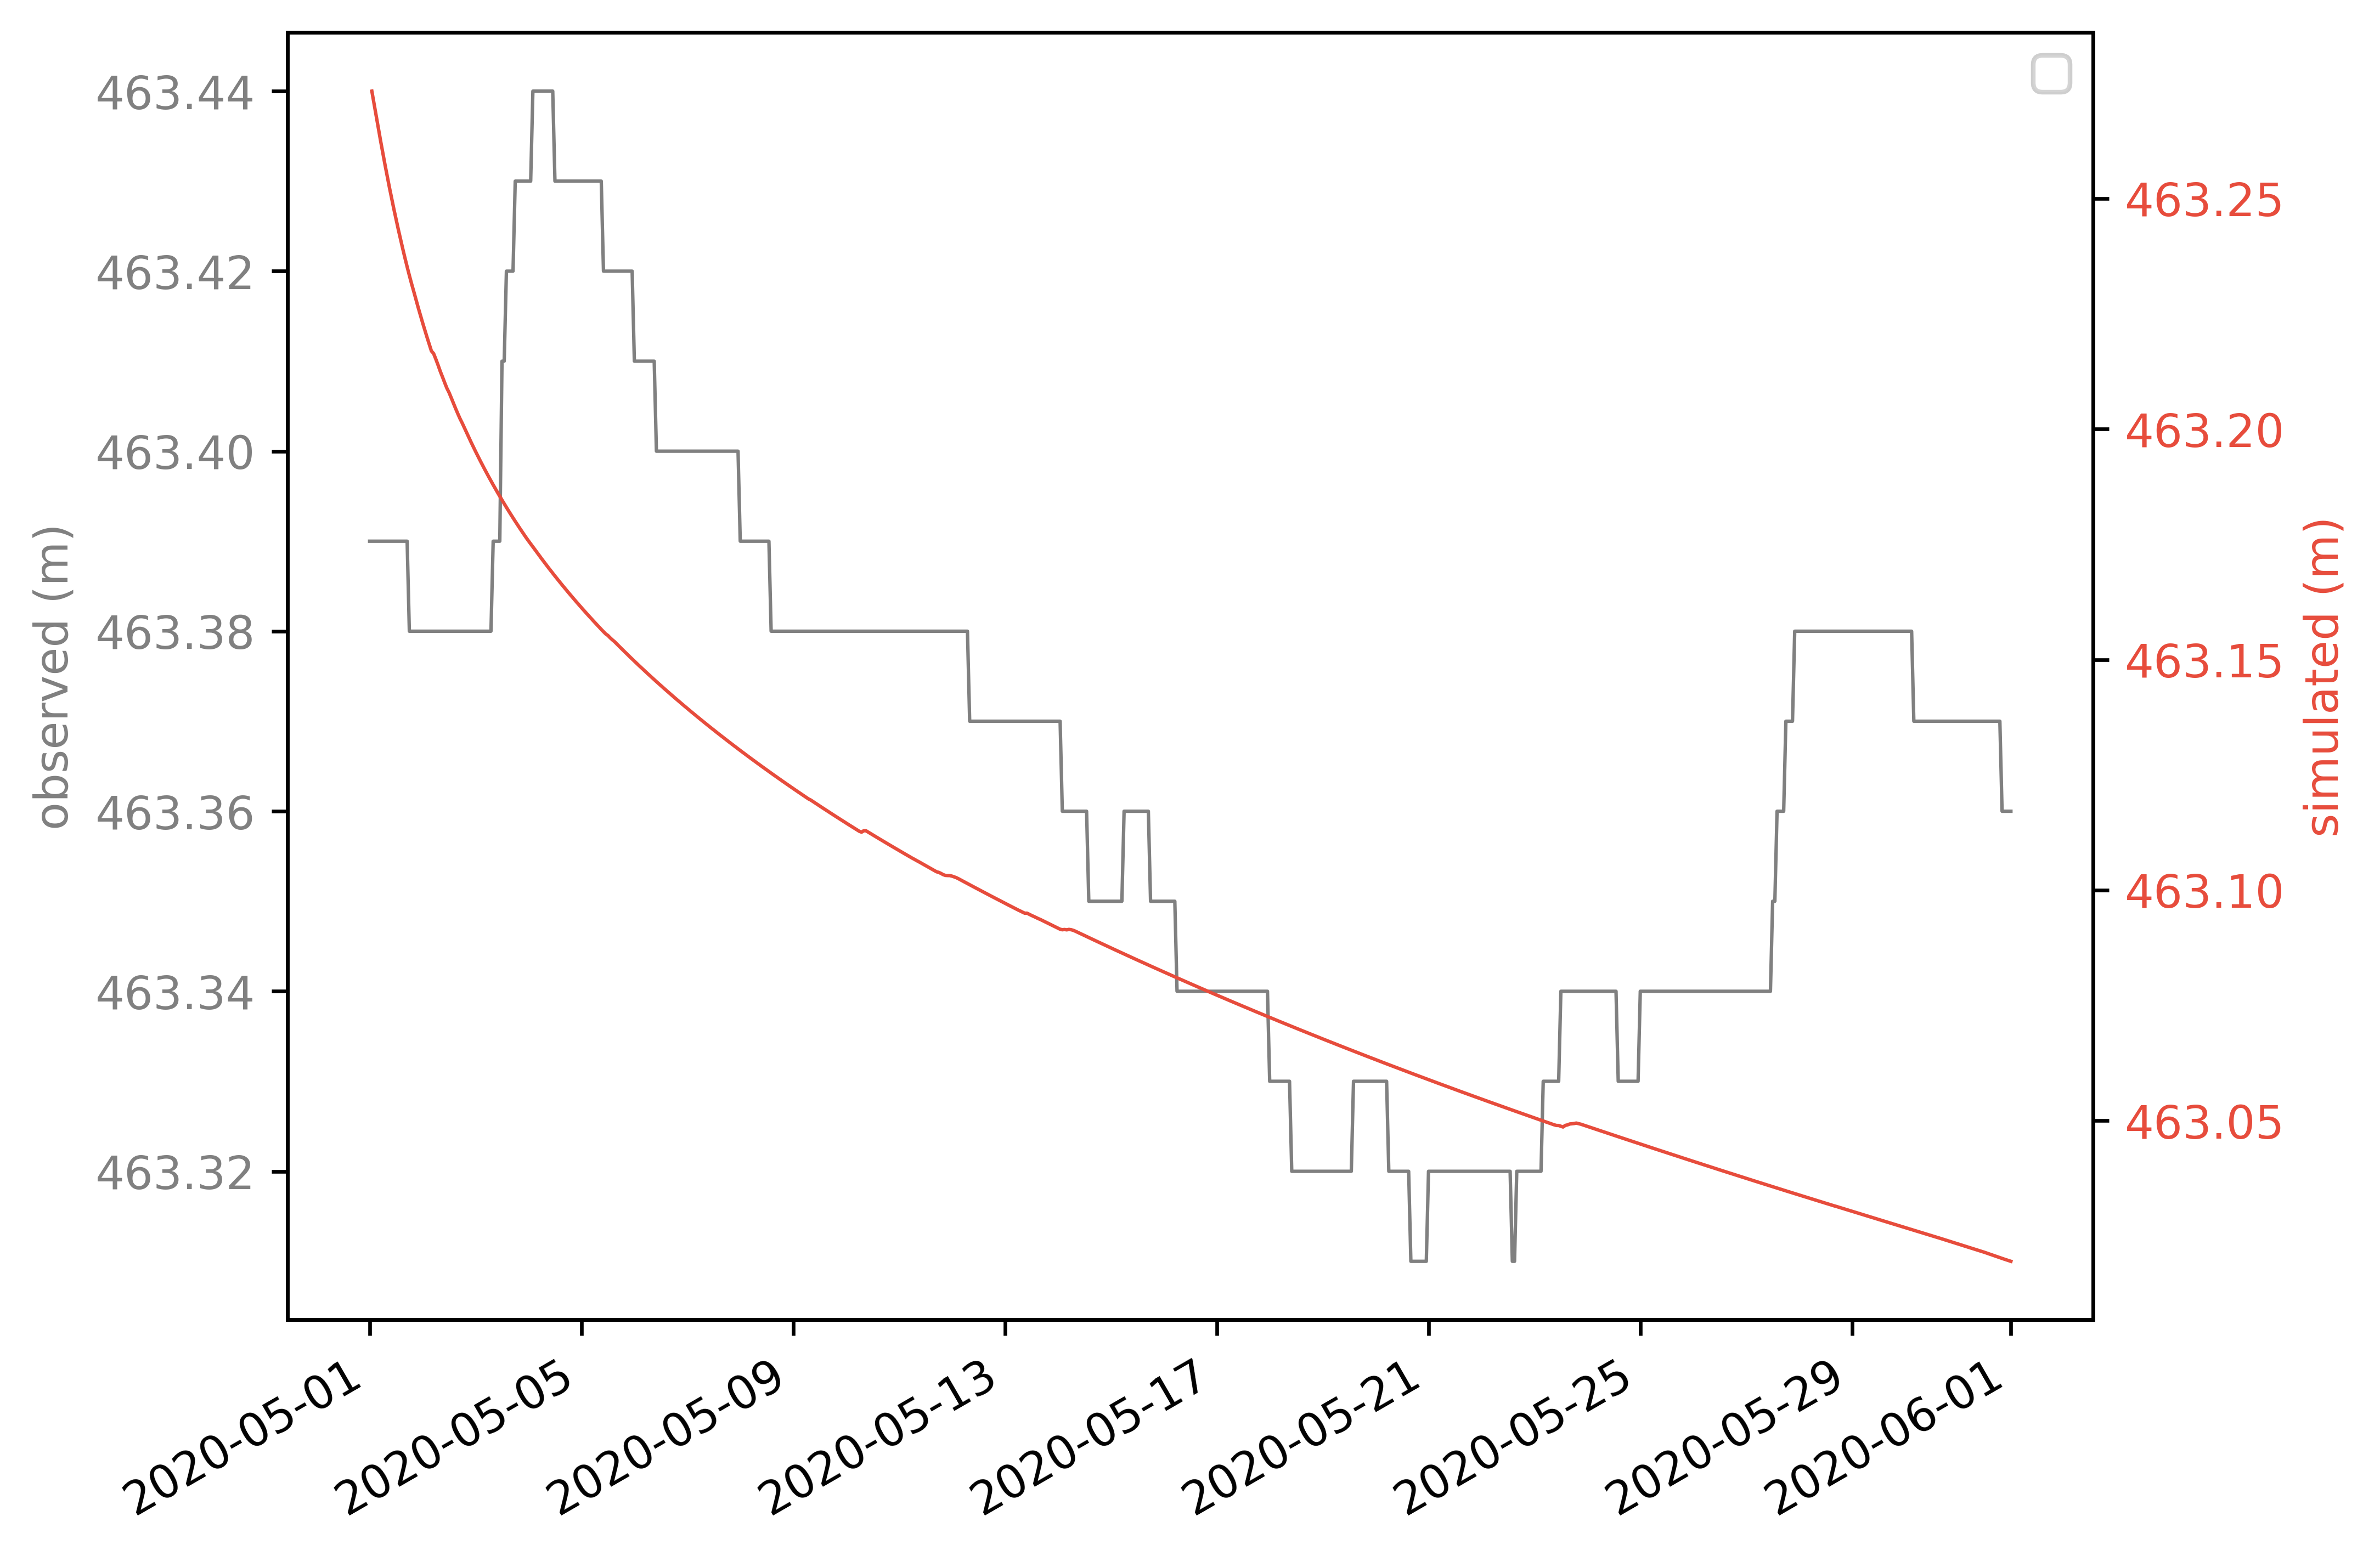
\includegraphics[height=0.42\textheight]{PICTURES/models_res/p1}
    \caption{Comparing simulated and measured observations at location P-1.}
    \label{fig:p1}
\end{figure}

\begin{figure}[H]
    \centering
    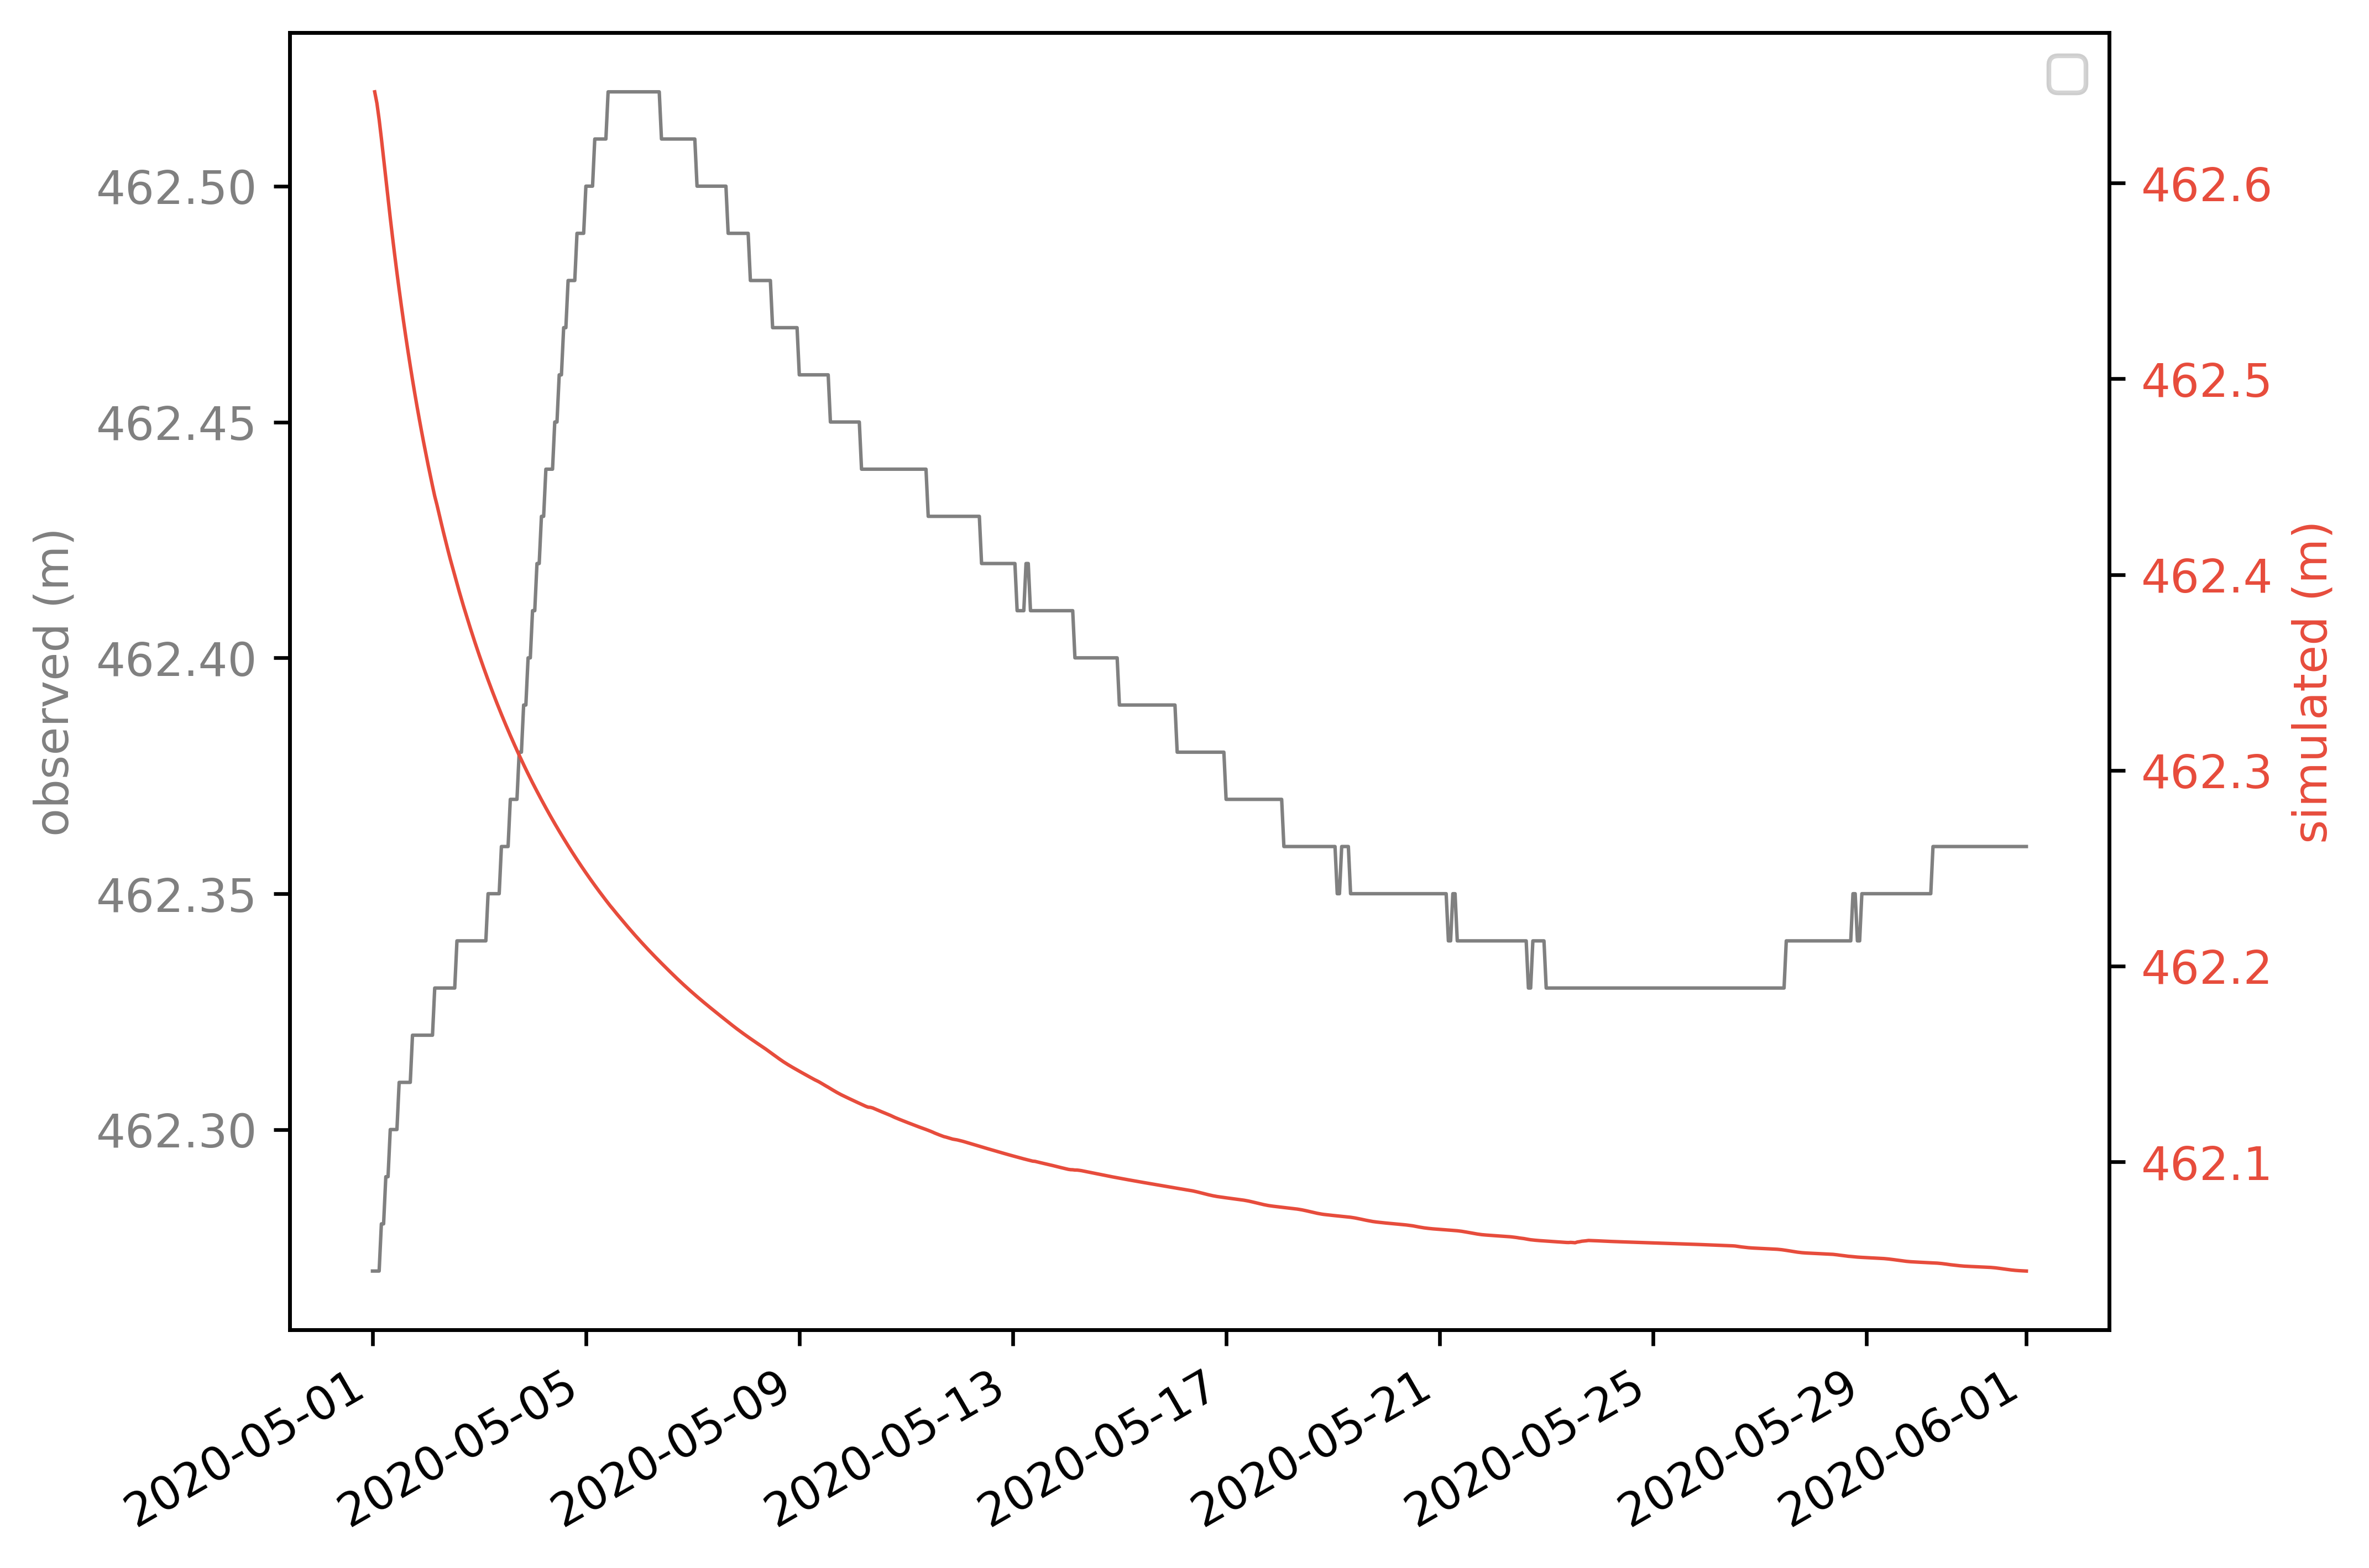
\includegraphics[height=0.42\textheight]{PICTURES/models_res/p12}
    \caption{Comparing simulated and measured observations at location P-12.}
    \label{fig:p12}
\end{figure}

\begin{figure}[H]
    \centering
    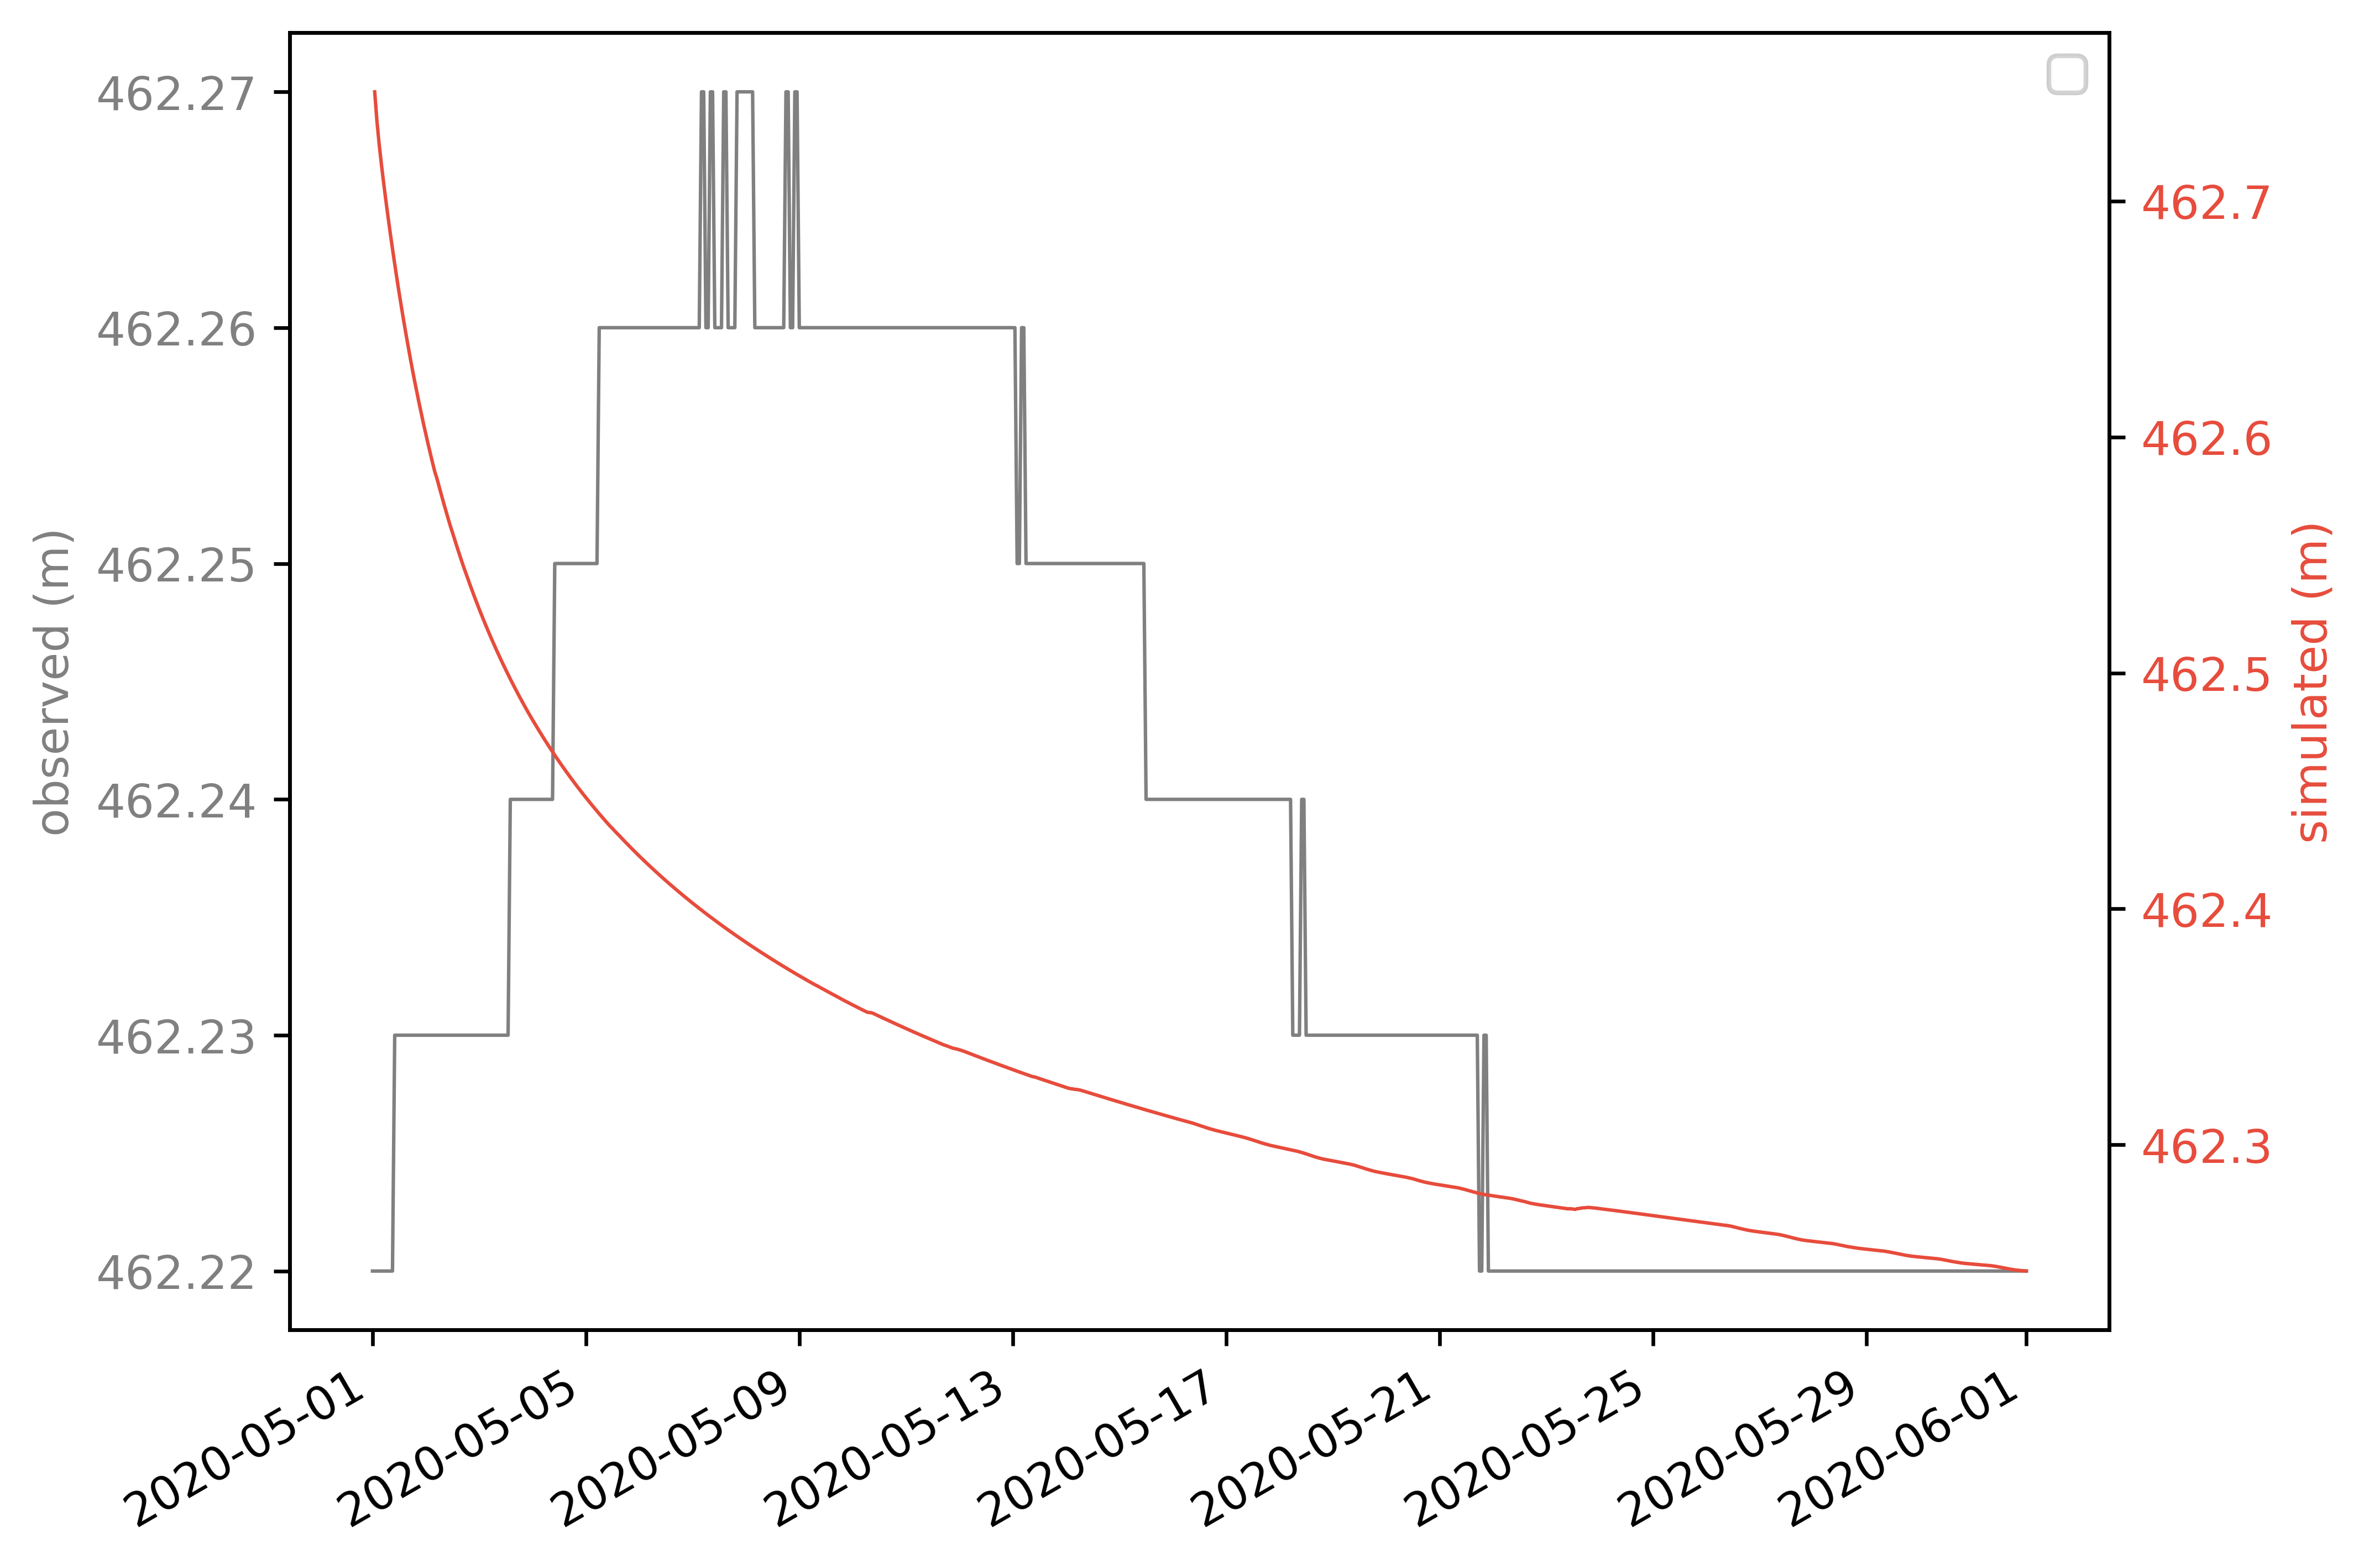
\includegraphics[height=0.42\textheight]{PICTURES/models_res/p6}
    \caption{Comparing simulated and measured observations at location P-6.}
    \label{fig:p6}
\end{figure}

\begin{figure}[H]
    \centering
    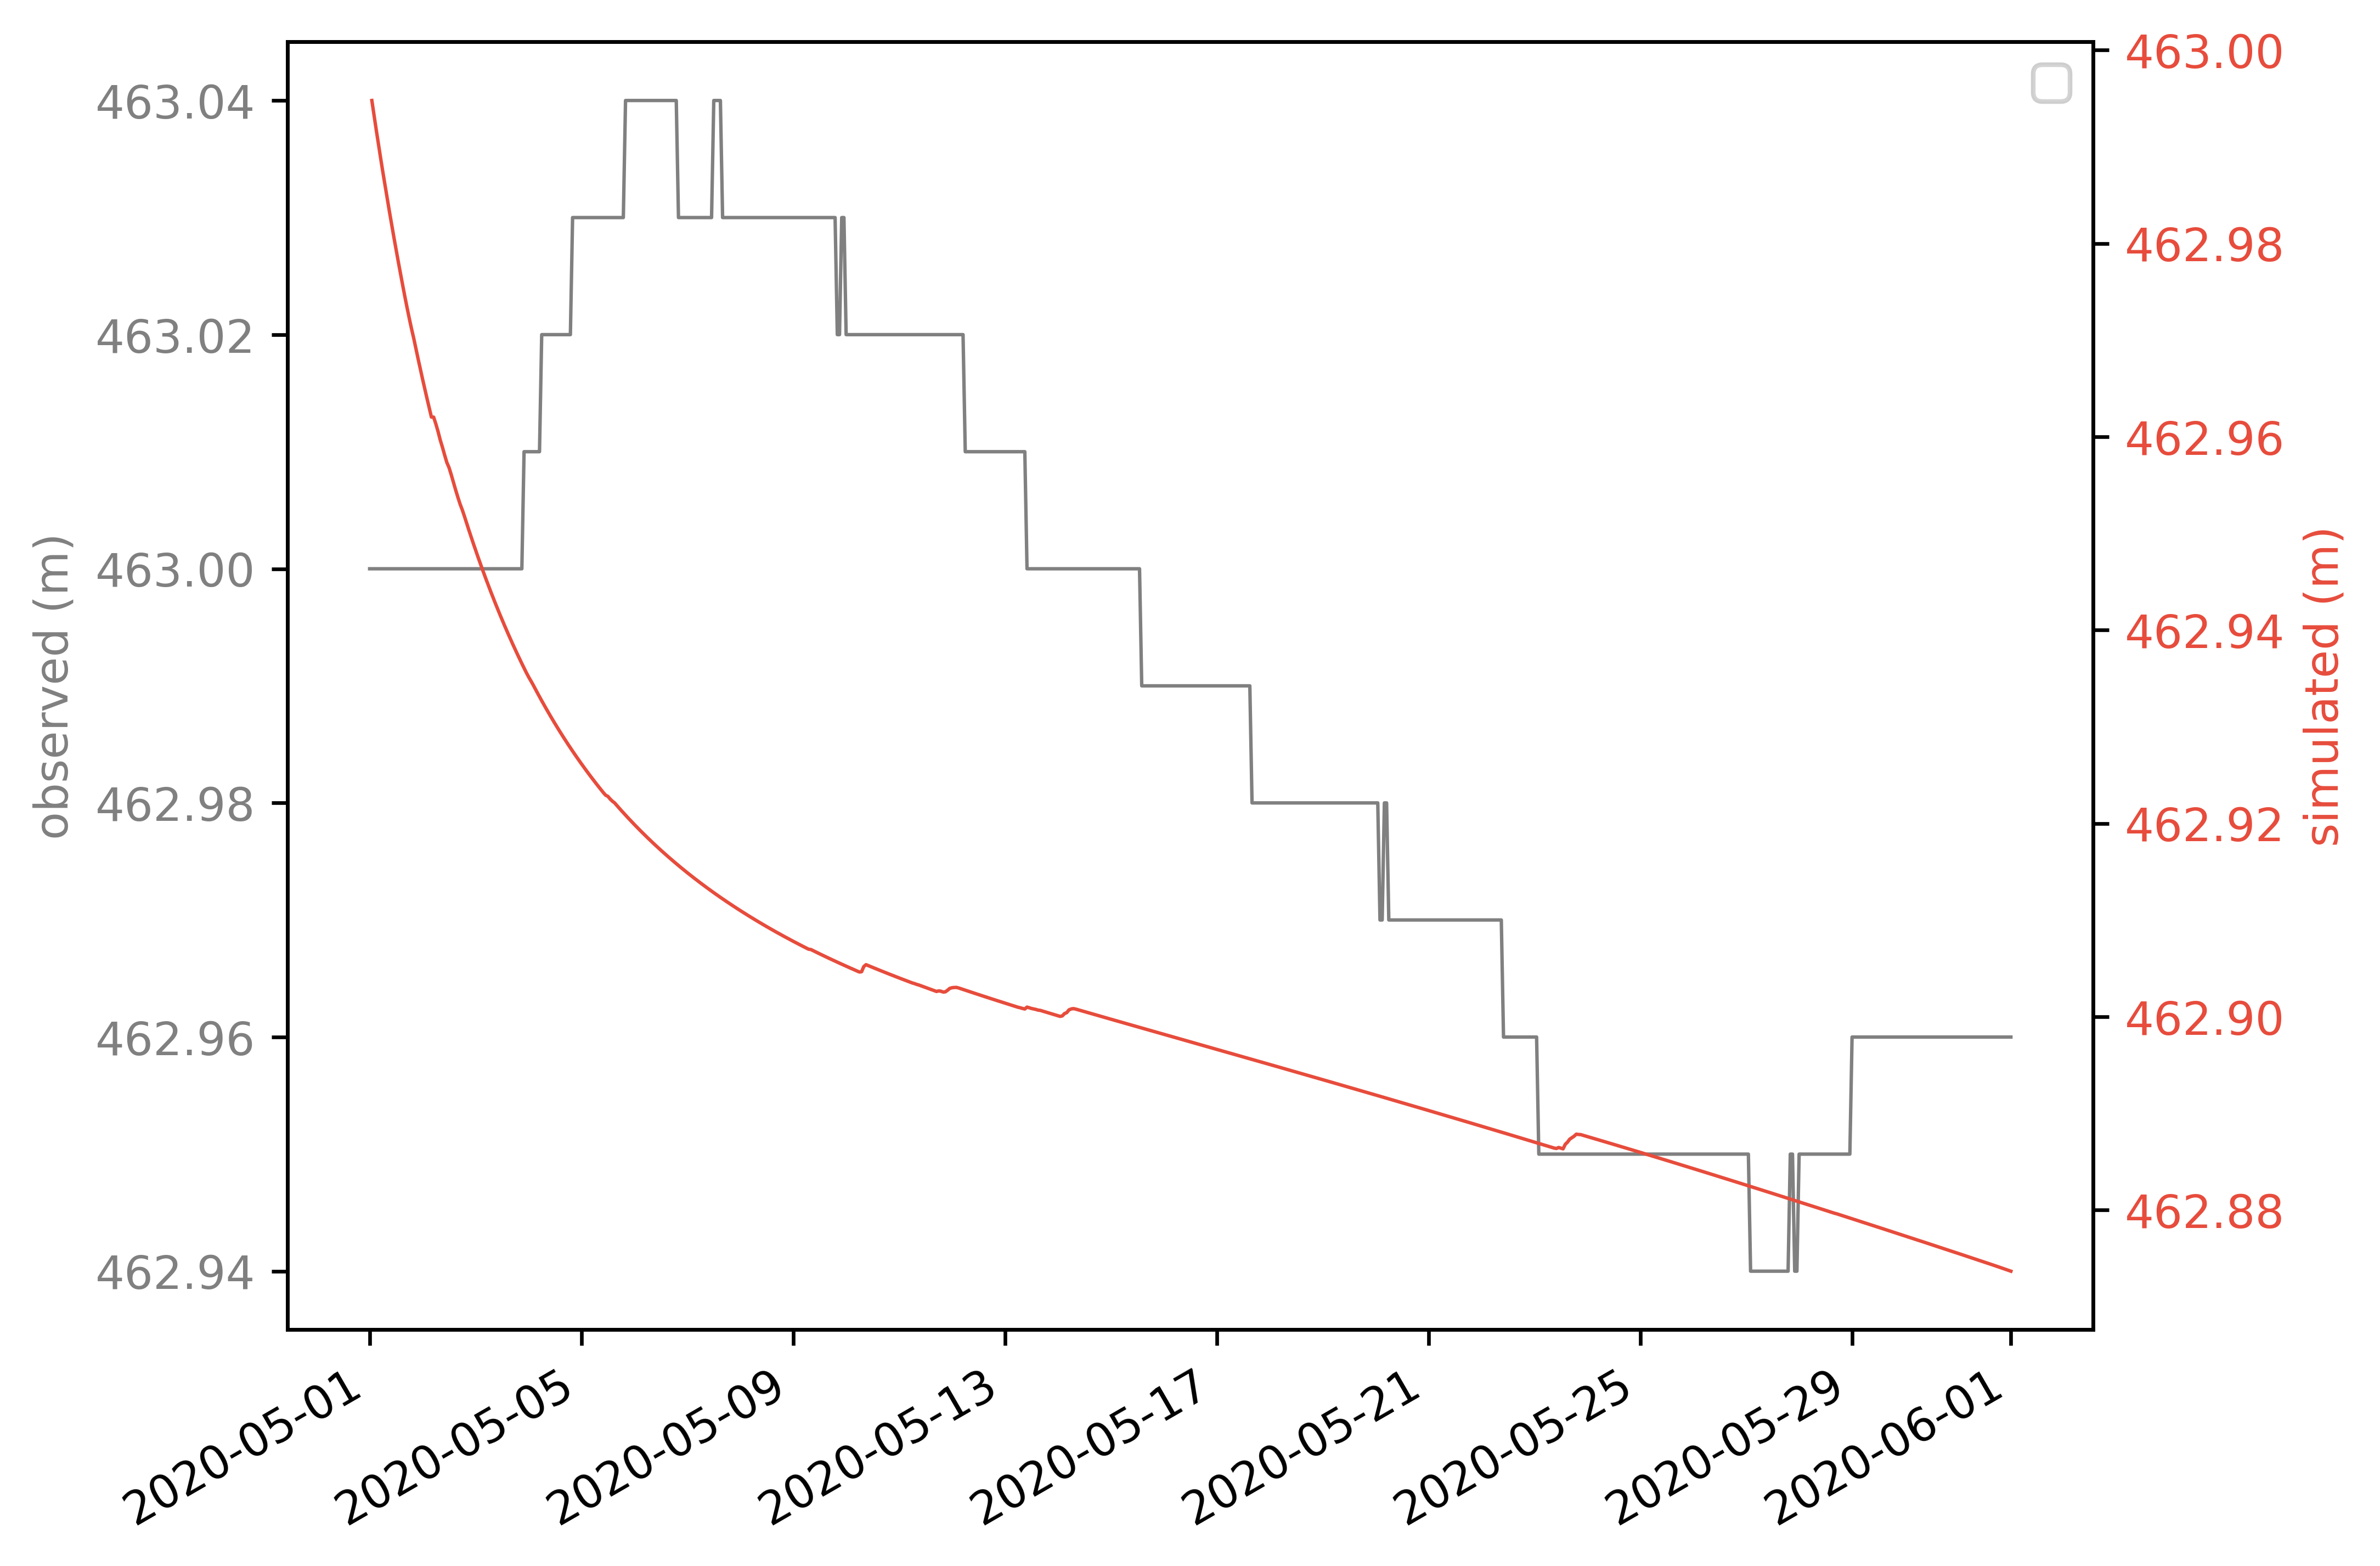
\includegraphics[height=0.42\textheight]{PICTURES/models_res/p7}
    \caption{Comparing simulated and measured observations at location P-7.}
    \label{fig:p7}
\end{figure}

\subsection{Addressing the Discrepancy}
One must note that the simulation set up was rather bare and is lacking in depth of representing the reality numerically. No calibration of either of the three models has been carried out. As discussed previously, GWSWEX model, being a conceptual model, demands extensive calibration. Furthermore, the initial conditions are very rough approximations that seem to be inadequately representative of the conditions observed in the study area. In this light, the simulated observations look rather quite promising.
\\ \\
The simulation may be improve with:
\begin{enumerate}
    \item calibration of GWSWEX, GW, and SW models,
    \item a better description of the GW model - especially the thickness of the unconfined zone,
    \item either improving the initial conditions to adequately represent the observed conditions in the study area, or running the simulation for a longer period of time and discarding the initial results to a point from where the measured and simulated observations agree quantitatively, adequately.
    \item improving the quality of P and ET inputs, and
    \item a finer temporal and spatial descretisization. 
\end{enumerate}

In the above list of improvements, Point (2) is crucial to the quality of the model results as the GWSWEX model heavily relies on the geometry to calculate GW and SM fluxes. It is known that the GW model used in this study does not have an adequately realistic representation of the study area as in some areas, as in observation locations P-2, P-1, and P-6, the model top in the GW model does not correspond to the measured elevations at these locations.
\\ \\
The study area lies almost in the middle of three meteorological stations. Thus, by combining  precipitation data from all three stations instead of using the data from just one (as is the case in this study) may further improve model results.
\\
Furthermore, the study enforced potential evapotranspiration directly. The model results might imitate the measured observations better if one enforced actual evapotranspiration instead.
\\ \\
The initial conditions are based purely on speculations from observing the measurements from the few observation locations that lie in the model domain. The relatively short simulation period of 1 month might not be adequate to allow the initial state of the model to achieve equilibrium. Thus, either a significantly longer simulation period and the assessment of the time scale at which the initial conditions no longer have an effect on the model results need to be determined for more reliable results.
\\ \\
For the sake of a testing and debugging, the simulation used coarse temporal and spatial descretisizations. The effects of varying temporal resolutions, which might be a crucial factor in explicit coupling schemes, are not studied. There is good scope for such a study.

\endinput
\chapter{Summary and Discussion}
\label{summary}
This study and, subsequently, its findings, have explored and successfully applied a novel, conceptual, 0-dimensional, numerical scheme to agreeably, qualitatively, describe the processes in the unsaturated zone  that can be used to couple existing groundwater (GW) and surface-water (SW) models to represent reality adequately for large-scale, distributed, GW-SW interactions. One must note, however, that the description of the processes in the unsaturated zone are extremely simplistic and conceptual descriptions of the complex process that occur in reality, constructed in an effort to leverage depth in description of these processes to maintain computational inexpensiveness; all while maintaining adequate depth in the description to produce usable results. The target applications for the model are scenarios that require a rudimentary depth-averaged estimation of the soil moisture in the unsaturated zone for relatively large model domains (above ~\SI{1000}{\metre\squared}). The proof-of-concept for the conceptualized model is established as it has demonstrated a good mass balance, as discussed in Section \ref{mass_balance}, alongside demonstrating the capability to simulate a scenario qualitatively close to the measured observations,  as discussed in Section \ref{obs}. To summarize:
\begin{itemize}
    \item the model demonstrated an acceptable mass balance when the quantum of in-/out- fluxes were compared against the changes in storage over each simulation period as described in Section \ref{mass_balance};
    \item the model produced, without any calibration and assumed initial conditions, simulated observations that were qualitatively comparable to the measured observations, as described in section \ref{obs}.
\end{itemize}

%\todo[inline]{H: I would say, this can be expanded a little to mention clearly (i) what has been done and (ii) what is the results. \\
%V: added the above itemized list to address this}

However, one must not overlook the following before applying the GWSWEX model and the coupling scheme:
\begin{itemize}
    \item The model is conceptual, i.e. it is only representative but not accurately descriptive of the underlying physics that it sets out to simulate and thus might not have the ability to capture a variety of nuances in these processes. One must be aware that this is by design, as such a conceptual simplification of the processes enable one to leverage the nuances in return for drastically cheaper computational costs. 
    \item The model produces depth averaged results while describing the unsaturated zone processes and estimating the soil moisture storage, i.e. it provides no qualitative or quantitative variations of the estimate along the vertical axis.
    \item Owing to the conceptual nature of the model, it demands extensive calibration to the application area.
\end{itemize}

During the study, it was realised that the following improvements may be made to the GWSWEX model:
\begin{itemize}
    \item Implementation of a numerical scheme to estimate and withdraw the actual evapotranspiration outflux based on the prescribed potential evapotranspiration, somewhat similar to how the incoming precipitation influx is allocated to the three storage terms.
    \item Enabling spatially variable precipitation and evapotranspiration inputs.
    \item Investigating the implementation of inter-cellular SM storage terms, possibly via a numerical scheme based on natural neighbor interpolation, to simulate unsaturated subsurface flows.
\end{itemize}


\endinput
%\include{TEXs/tipsandtricks}



%% BIBLIOGRAPHY
\pdfbookmark[0]{Bibliography}{Bibliography}
\bibliographystyle{LITERATURE/lf_gb_ila_vt}
% \bibliographystyle{plain}
\bibliography{LITERATURE/thesis_references}

\begin{appendix}
\definecolor{codegreen}{rgb}{0,0.6,0}
\definecolor{codegray}{rgb}{0.5,0.5,0.5}
\definecolor{backcolour}{rgb}{0.95,0.95,0.92}

\lstset{
    numbers=left,
    breaklines=true,
    tabsize=2,
    basicstyle=\ttfamily\footnotesize,
    backgroundcolor=\color{backcolour},   
    commentstyle=\color{codegreen},
    keywordstyle=\color{blue},
    numberstyle=\tiny\color{codegray},
    stringstyle=\color{magenta},
    literate={\ \ }{{\ }}1
}

\chapter{The GWSWEX Model}
\label{GWSWEX_program}
\lstinputlisting[language=Fortran]{LITERATURE/GWSWEX.f90}


\chapter{The GWSWEX Python Module}
\label{GWSWEX_module}
The following program demonstrates the use of the GWSWEX module, within which the coupling scheme is implemented. The module itself may be accessed at \url{https://github.com/Veethahavya/GWSWEX}.

\lstinputlisting[language=Python]{LITERATURE/GWSWEX_run.py}


\endinput
\end{appendix}

\end{document}